\chapter{\texorpdfstring{\MakeUppercase{Measuring Turbulence in the Interstellar Medium with Young Stars}}{Measuring Turbulence in the Interstellar Medium with Young Stars}}
\label{chap:stars}


\begin{figure}[b]
    \centering
    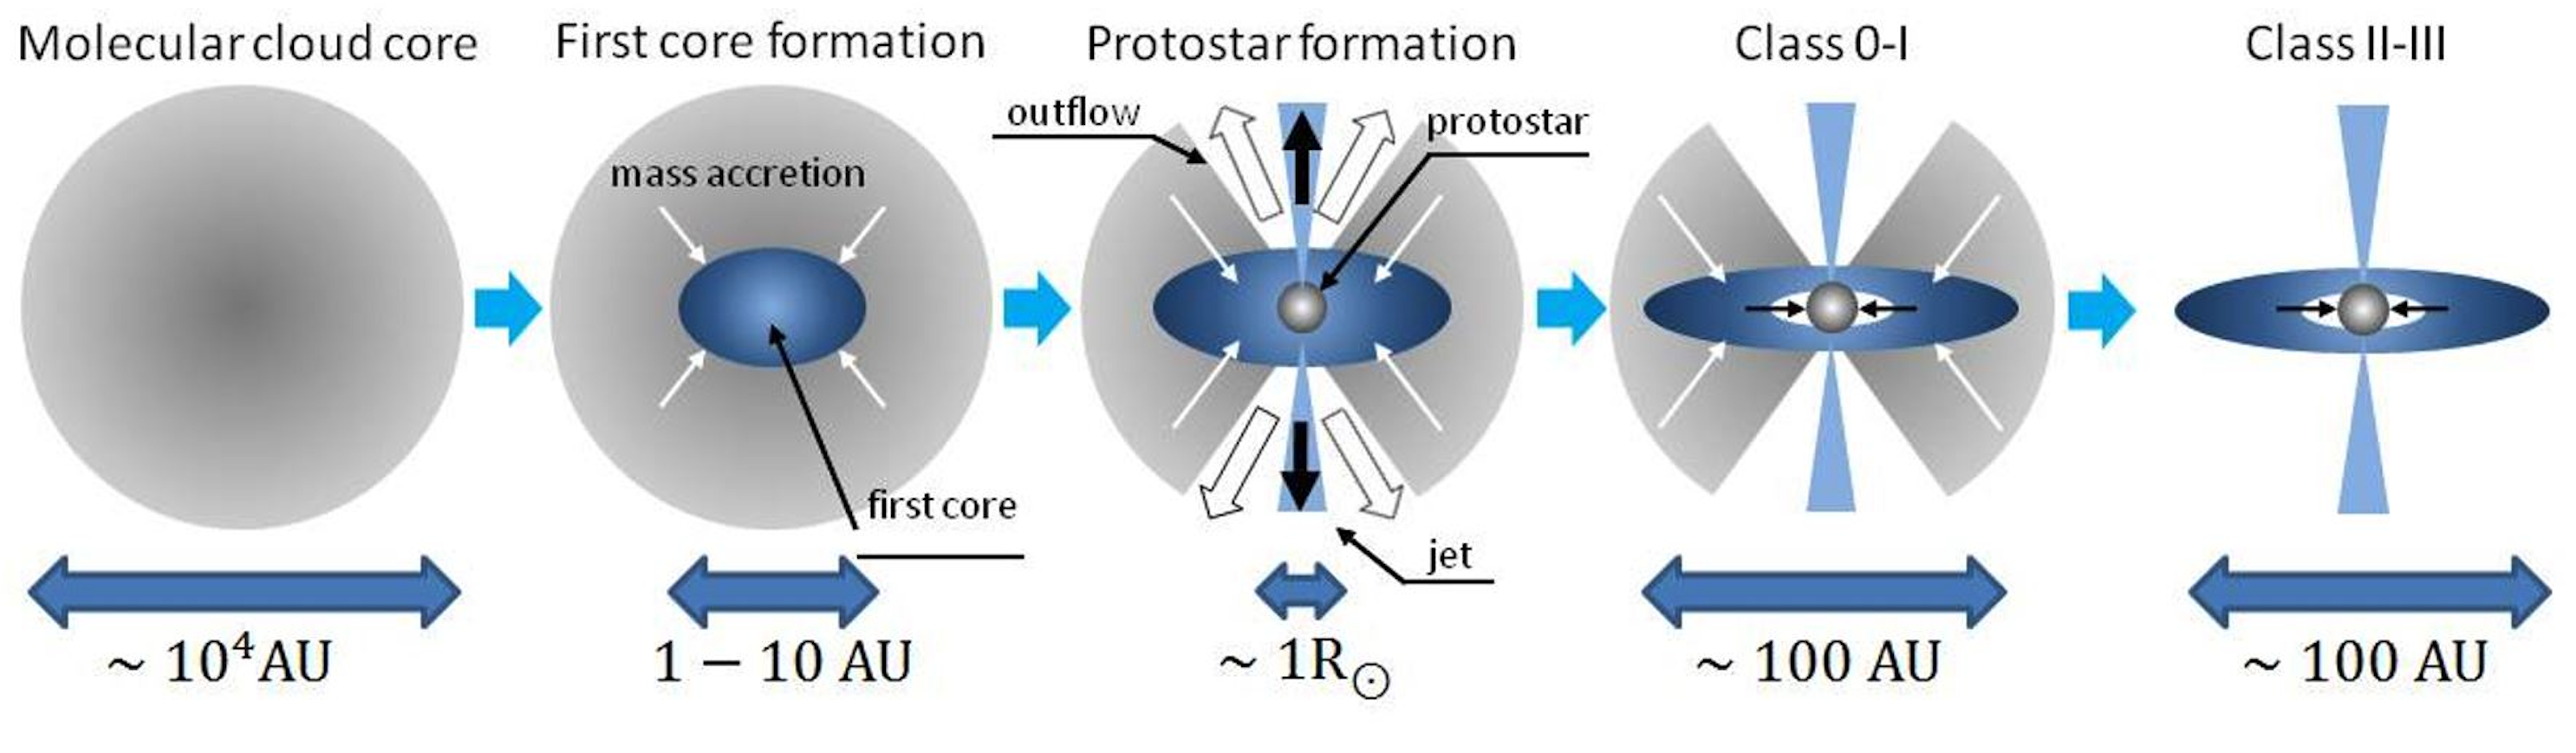
\includegraphics[width=0.8\linewidth]{Stars_img/star_formation_illustration.png}
    \caption[Illustration of the star formation process.]{Illustration of the star formation process. Credit: Yusuke Tsukamoto, RIKEN.}
    \label{fig:star-formation}
\end{figure}

Inside the interstellar medium (ISM), molecular clouds are sites of star formation.
The densest parts of these clouds, the \textit{molecular cores}, undergo gravitational collapse to form stars (see Figure~\ref{fig:star-formation}). 
It is well known that the ISM is multiphase and turbulent \citep{mckee_theory_2007}.
\cite{larson_turbulence_1981} investigated the kinematic properties of various molecular clouds within the Milky Way, and found a power-law relation between the velocity dispersion and cloud size, indicative of a Kolmogorov-like turbulent cascade in the local universe. 
Previously, turbulence in the ISM has been detected and analyzed using a variety of gas tracers.
The warm-ionized phase can be probed with \halpha\ \citep{haffner_wisconsin_2003}, the warm-neutral medium with \ion{H}{1} \citep[e.g.,][]{burkhart_characterizing_2009}, the cold molecular phase with CO, HCO, NH$_3$, etc. \citep[e.g.,][]{turner_physics_1997,qian_13co_2012,heyer_universality_2004}.
In these studies, the line-of-sight velocities at individual angular positions are measured by computing the Doppler shift of the emission/absorption line.
These tracers provide extremely reliable measurements, but fail to describe a complete picture of the local velocity field, lacking one spatial dimension and two velocity dimensions.
Thus, measurements of turbulence often suffer from projection effects that are difficult to correct for \citep{qian_new_2015}.

In \citet[][]{ha_measuring_2021} and \citet[][]{ha_turbulence_2022}, we proposed a new method to probe turbulence in star-forming regions of the Milky Way.
Since stars form out of turbulent molecular cores, we hypothesized that the newly born stars could \textit{inherit} the turbulent kinematics of their natal clouds.
To test this theory, we utilized six-dimensional (6D) kinematic measurements of young stars in Orion \citep{ha_measuring_2021}, Ophiuchus, Perseus, and Taurus \citep{ha_turbulence_2022} from the Gaia \citep{collaboration_gaia_2016,brown_gaia_2021} and APOGEE-2 \citep{blanton_sloan_2017} surveys.
If young stars were good tracers of turbulence in the ISM, we predicted that the usual characteristics of turbulence (i.e., a statistically coherent motion) would also be seen in their astrometries.
This procedure also gave us access to a complete kinematic picture of young stars in these regions, bypassing limitations imposed by projection effects.

In the following studies, we measured the level of turbulence in each region using a technique called the velocity structure function (VSF).
The VSF is related to the kinetic energy power spectrum of a velocity field, and is expressed as a two-point correlation function relating the absolute velocity differences $|\delta v|$ to the physical separation $\ell$. For a turbulent velocity field, the VSF follows a characteristic power-law scaling, $|\delta v| \propto \ell^k$, with slope $k = 1/3$ for incompressible turbulence dominated by solenoidal motions \citep[][]{kolmogorov_local_1941}, or a slope $k = 1/2$ for supersonic turbulence dominated by compressive motions \citep{burgers_mathematical_1995}. For the Milky Way molecular clouds, \citet{larson_turbulence_1981} found a relationship between cloud size and velocity dispersion to be $\sigma = 1.1~R^{0.38}$.

The following sections are adapted from \citet{ha_measuring_2021}, the Astrophysical Journal Letters, 907, L40, and \citet{ha_turbulence_2022}, the Astrophysical Journal, 934, 7.

\section{The Signal of Turbulence from Young Stars in the Orion Complex}

\publicationdetails
{Ha et al. 2021, ApJL, 907, L40}
{Trung Ha\footnotemark[1], Yuan Li\footnotemark[1]\footnotemark[2], Siyao Xu\footnotemark[3]\footnotemark[7], Marina Kounkel\footnotemark[4], and Hui Li\footnotemark[5]\footnotemark[6]\footnotemark[7]}
{Stars form in molecular clouds in the interstellar medium (ISM) with a turbulent kinematic state. Newborn stars therefore should retain the turbulent kinematics of their natal clouds. Gaia DR2 and APOGEE-2 surveys in combination provide three-dimensional (3D) positions and 3D velocities of young stars in the Orion Molecular Cloud Complex. Using the full 6D measurements, we compute the velocity structure functions (VSFs) of the stars in six different groups within the Orion Complex. We find that the motions of stars in all diffuse groups exhibit strong characteristics of turbulence. Their first-order VSFs have a power-law exponent ranging from $\sim0.2$--$0.5$ on scales of a few to a few tens of parsecs, generally consistent with Larson's relation. On the other hand, dense star clusters, such as the Orion Nebula Cluster (ONC), have experienced rapid dynamical relaxation, and have lost the memory of the initial turbulent kinematics. The VSFs of several individual groups and the whole Complex all show features supporting local energy injection from supernovae. The measured strength of turbulence depends on the location relative to the supernova epicenters and the formation history of the groups. Our detection of turbulence traced by young stars introduces a new method of probing the turbulent kinematics of the ISM\@. Unlike previous gas-based studies with only projected measurements accessible to observations, we utilize the full 6D information of stars, presenting a more complete picture of the 3D interstellar turbulence.}
{\footnotetext[1]{Department of Physics, University of North Texas, Denton, TX 76203, USA}
\footnotetext[2]{Department of Astronomy, University of California, Berkeley, CA 94720, USA}
\footnotetext[3]{Institute for Advanced Study, 1 Einstein Drive, Princeton, NJ 08540, USA}
\footnotetext[4]{Department of Physics and Astronomy, Western Washington University, 516 High St, Bellingham, WA 98225, USA}
\footnotetext[5]{Department of Physics, Kavli Institute for Astrophysics and Space Research, Massachusetts Institute of Technology, Cambridge, MA 02139, USA}
\footnotetext[6]{Department of Astronomy, Columbia University, 550 West 120th Street, New York, NY 10027, USA}
\footnotetext[7]{NASA Hubble Fellow}}

\subsection{Introduction}
\label{sec:orion-intro} 
\setcounter{footnote}{0} 
The interstellar medium (ISM) is turbulent. More specifically, the cold dense star-forming molecular clouds are turbulent. For example, \citet{larson_turbulence_1981} finds a power law relation between velocity dispersion and cloud size with an exponent of 0.38, similar to the Kolmogorov law for incompressible turbulence \citep{kolmogorov_local_1941}. Turbulence plays an important role in regulating the cloud dynamics and star formation \citep{mac_low_control_2004, mckee_theory_2007,hennebelle_turbulent_2012},
from cloud scales all the way down to the scales much smaller than molecular cores 
\citep{hull_unveiling_2017}.

The ubiquitous interstellar turbulence induces velocity fluctuations on all scales in both diffuse interstellar phases and dense star-forming gas. Statistical measurements of velocity fluctuations in the multiphase ISM can be done using the Velocity Channel Analysis (VCA), the Velocity Coordinate Spectrum (VCS) \citep{lazarian_velocity_2000,lazarian_studying_2006}, the Delta-variance technique \citep{ stutzki_fractal_1998,ossenkopf_turbulent_2002}, or the Principal Component Analysis \citep{ heyer_universality_2004,roman-duval_turbulence_2011} based on spectroscopic data.
These analyses generally reveal power-law spectra of turbulent velocities \citep{ lazarian_obtaining_2009,chepurnov_velocity_2010}.

Many processes can drive turbulence in the ISM, such as gravity, shear, and various forms of stellar feedback including supernova explosions \citep{krumholz_is_2016,padoan_supernova_2016}. Turbulent motions shape the filamentary density structures in molecular clouds (e.g., \citealt{ federrath_universality_2016,xu_formation_2019}). Dense cores and protostars subsequently form in dense filaments \citep{andre_interstellar_2017}.

Besides gas tracers that are commonly used to probe turbulence in the 
volume filling ISM, 
turbulent velocities can also be sampled using point sources 
such as molecular cores formed at the density peaks generated in highly supersonic turbulence. 
For example, \citet{qian_13co_2012} developed statistical measurements of 
core-to-core velocity dispersion over a range of length scales, i.e.,
the core velocity dispersion technique. \citet{qian_studies_2018} find 
signatures for a turbulent power-law spectrum in the Taurus Molecular Cloud, and demonstrate that the statistics of turbulent velocities are imprinted in the velocities of dense cores \citep{xu_projected_2020}. 

Because prestellar cores are nurseries of stars, newborn stars should naturally inherit the velocities of cores and hold the fossil information on the turbulent velocities of their natal clouds, as long as dynamical interactions of young stars have not erased that information.

In this work, we carry out the first statistical analysis of star-to-star velocity structure function (VSF) across the Orion complex over a range of length scales, from $\sim200$ pc down to $<1$ pc. These newly formed stars are expected to still ``remember" the local gas kinematics at their birth, and can be used to recover the turbulent motions in the parent cloud. With direct measurements on 3D velocities and 3D positions, the statistical study of turbulent velocities with stars do not suffer from the 
complex convolution between density and velocity and the projection effect as that with the commonly used gas tracers. 

In Section~\ref{sec:data}, we describe the data used in this analysis and how we compute the VSFs. We present the VSF for each group in the Orion complex in Section~\ref{sec:orion-results}, and discuss how the slope and amplitude is related to the location and history of the stellar system. In Section~\ref{sec:discussions}, we discuss the uncertainties and biases of the analysis, and how our method and results compare with previous works on turbulence in the ISM.


\subsection{Data Processing}\label{sec:data}

\begin{figure}
    \centering
    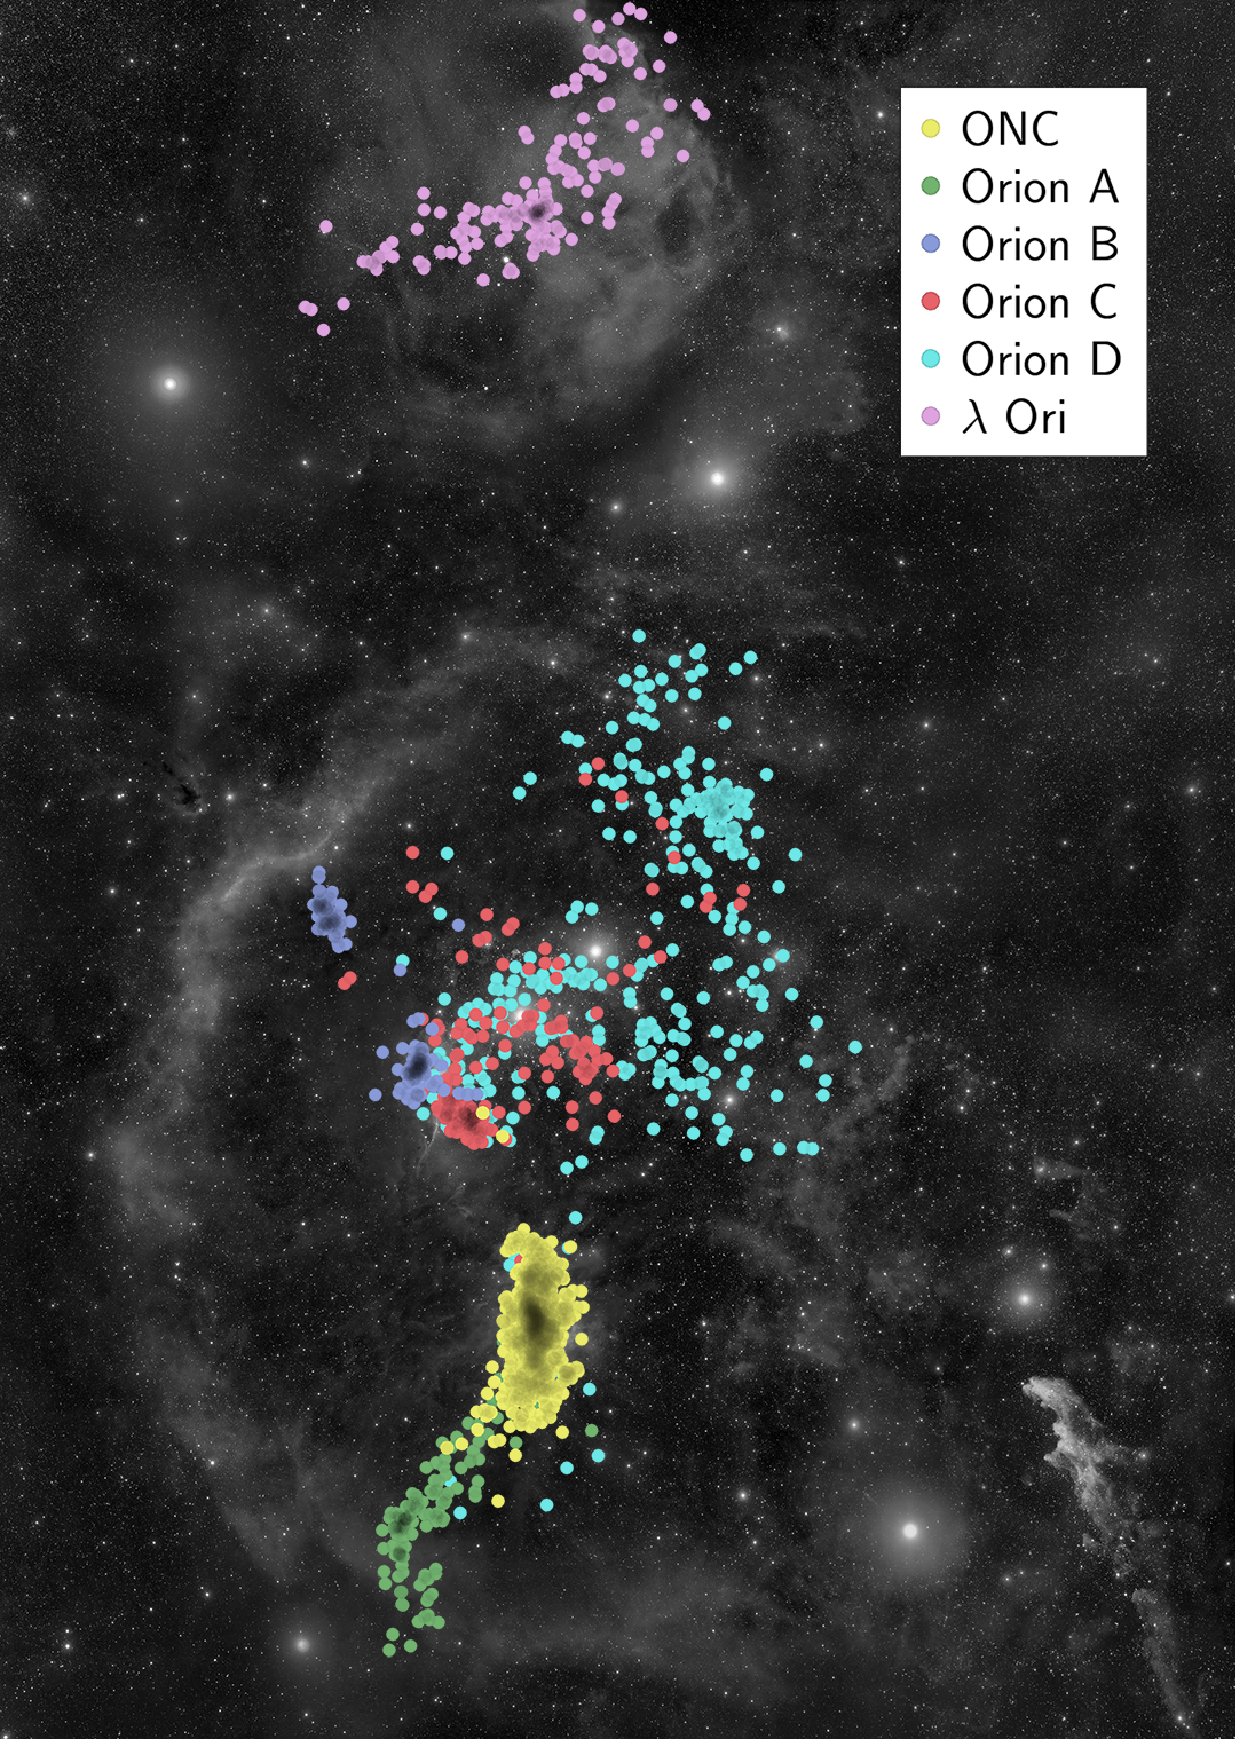
\includegraphics[width=0.8\linewidth]{Stars_img/orion_overlay.pdf}
    \caption{Foreground: each dot represents the projected position of a star in the Orion Complex that we include in our analysis. The star's color corresponds to its main group. Background: greyscale optical image of the Orion Molecular Cloud Complex, courtesy of Rogelio Bernal Andreo.}
    \label{fig:orion}
\end{figure}

\subsubsection{Data Acquisition}\label{sec:data1}
We obtain the locations, parallax distances, and proper motions of stars in the Orion Molecular Cloud Complex from Gaia's second data release \citep{gaia_collaboration_gaia_2018}. The Gaia catalog includes five-parameter astrometric data from over 1.3 billion stars. 
The line-of-sight velocities of the stars were observed in the near infrared during the Apache Point Observatory Galactic Evolution Experiment 2 (APOGEE-2). The APOGEE spectrograph is mounted on the 2.5 m Sloan Foundation Telescope of the Sloan Digital Sky Survey (SDSS), and is used to collect high resolution spectral images of over 400,000 stars in the Milky Way \citep{gunn_25_2006,blanton_sloan_2017}. 
In total, 8891 stars from APOGEE-2, and 16754 stars from Gaia DR2 were observed towards the Orion Complex, as specified by \citet{kounkel_apogee-2_2018}. Combining these two surveys provides six-dimensional information of a subset of stars.

\citet{kounkel_apogee-2_2018} developed a hierarchical clustering algorithm to assess membership of the Orion Complex and its structure based on the position of stars in the phase space (position+velocity). They identify five main groups inside the Complex, namely Orion A, Orion B, Orion C, Orion D, and $\lambda$ Ori. We require all stars in our sample to be a part of one of these groups, excluding all of the stars that could not be clustered together (i.e., field stars, or other members of Orion that may have peculiar velocity---such as spectroscopic binaries or runaways). Furthermore, we require a complete information on six-dimensional position and velocity for each star, i.e., a star needs to have both astrometric solutions from Gaia DR2 as well as radial velocities from APOGEE\@. Through this, we obtain a sample of 1439 stars.

We note that the Orion Nebula Cluster (ONC) is a part of the Orion A molecular cloud, however, it is very unique, being a singularly most massive young cluster in the solar neighborhood. The environment that is found in the ONC is different from the more diffuse environment in the southern part of Orion A. Thus, for the purpose of our analysis, we separate ONC and the rest of the Orion A. Throughout the paper, Orion A refers only to the ``tail'' of the cloud (L1641 and L1647), excluding stars in ONC\@. The reasoning behind this split is discussed in Section~\ref{sec:orion-results}. The term ``group'' in this paper refers to all ``stellar systems'' that are spatially and kinematically associated, while ``cluster'' only refers to open clusters such as the ONC.

Table~\ref{table:data} lists the number of stars and the mean age of each main group and the ONC\@. We plot the projected positions of the stars in our analysis over a greyscale image of the Orion Complex in Figure~\ref{fig:orion}.


\subsubsection{Method of analysis}\label{sec:orion-method}
\begin{figure*}
    \centering
    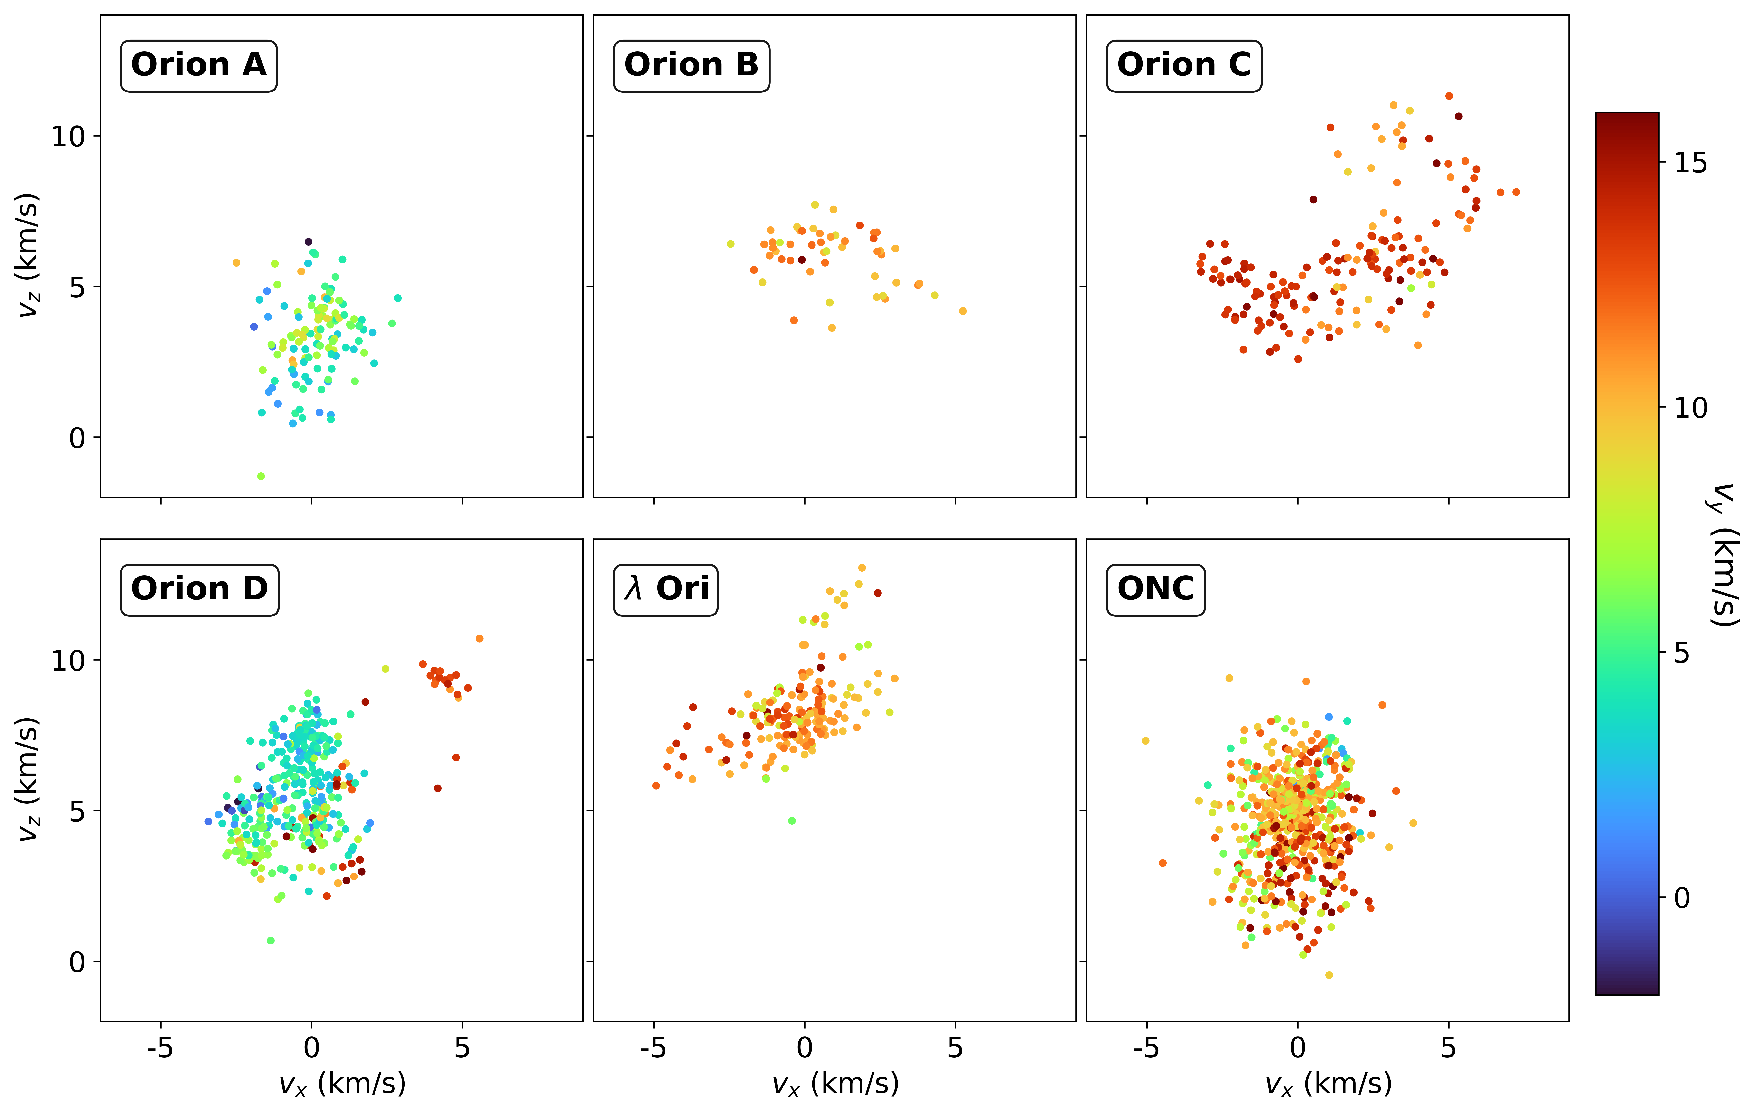
\includegraphics[width=0.98\linewidth]{Stars_img/allVelocities.pdf}
    \caption{Velocities of stars in the six clouds in our analysis in Cartesian coordinate. The color map denotes stars' velocity in the y direction, which closely resembles their radial velocity. All clouds show some level of randomness in the velocities of the stars.}
    \label{fig:velodist}
\end{figure*}
To test our hypothesis that young star clusters ``remember" their local gas kinematics at the time of birth, we compute the VSFs for all identified groups, as well as the VSF of the combined Orion Complex catalog, both with and without the ONC\@. We first convert the radial velocity and proper motion of stars into velocity in Cartesian coordinate, in the Local Standard of Rest (LSR). Figure~\ref{fig:velodist} shows the 3D velocity information of stars used in this study in each cloud.

For each cloud, we compute the first-order VSF and its uncertainties. The VSF for a sample of stars can be calculated in the following way: for each pair of stars, we first record the physical separation $\ell$ of the pair and compute the magnitude of the vector velocity difference $\delta \Vec{v}$ as the velocity difference $|\delta v|$. We then compute the average of the velocity differences $\langle |\delta v| \rangle$ within logarithmic bins of $\ell$. 

The VSF is related to the kinetic energy power spectrum of turbulence. It describes how velocity difference ($|\delta v_{ij}|$) relates to the physical separation ($\ell_{ij}$) for given pairs of points in space ($i$, $j$). In a turbulent flow, kinetic energy cascades down from large scales to small scales, and the velocity differences become smaller toward smaller scales. If the turbulence is incompressible (subsonic), we expect the first-order VSF to be $|\delta v_{ij}|\sim \ell_{ij}^{1/3}$ within the inertial range \citep{kolmogorov_local_1941}. For compressible (supersonic) turbulence, $|\delta v_{ij}|\sim \ell_{ij}^{1/2}$ \citep[e.g.,][]{federrath_universality_2013}.

To estimate uncertainties of the VSF, we first perform random sampling of the measurements of stars' properties based on the observed uncertainties, and obtain 1000 realizations for each star following a Gaussian distribution. We only consider measurement uncertainties of the parallax distances, proper motions, and radial velocities. We ignore the uncertainties in RA and Dec because they are typically much smaller than the uncertainties of other quantities. For each group, we then obtain 1000 VSFs, with each iteration excluding a random star within the group. This allows us to account for both measurement errors and uncertainties due to small sampling sizes in some bins of $\ell$. We take the mean and standard deviation of the computed VSFs to be the group's VSF and its corresponding error. We choose 1000 iterations to ensure accuracy even though the results are already converged at 100 iterations. We also compute the second and third-order VSFs of the groups, and discuss them in Section~\ref{subsec:high_order}.

\begin{sidewaystable}
    \centering
    \caption{Properties of molecular clouds in the Orion Complex}
    \label{table:data}
    \begin{tabular}{ccccccc}
        \toprule
                              & Orion A   & Orion B  & Orion C  & Orion D   & Lambda Ori & ONC      \\
        \midrule
        Number of Stars$^a$   & 117       & 51       & 162      & 354       & 170        & 585      \\
        Median Age (Myr)      & 2.2       & 1.3      & 4.1      & 4.9       & 3.7        & 2.7      \\
        Crossing Time (Myr)   & 16.1      & 13.6     & 8.0      & 12.9      & 12.8       & 6.9$^b$  \\
        Fitting Range$^c$ (pc)& 10--90  & 8--60  & 9--50  & 15--58  & 10--32   & 5--40  \\
        Slope of VSF          & $0.18$    & $0.14$   & $0.19$   & $0.53$    & $0.36$     & $0.05$   \\
        \bottomrule
    \end{tabular}
    \parbox{\linewidth}{\footnotesize \textit{Note.} $^a$ Number of stars obtained 
    from the combined Gaia DR2 and APOGEE surveys with full 6D information 
    (Section~\ref{sec:data1}). $^b$ This is the crossing time for the entire ONC 
    cluster. The inner core has a much shorter crossing time and relaxation time 
    \citep{hillenbrand_preliminary_1998}. $^c$ The slope of the VSFs depends on the exact range 
    of separation taken into account. We choose the fitting range such that the 
    uncertainties are low and there is a consistent trend in the slope of the VSF.}
\end{sidewaystable}


\begin{figure*}
\centering
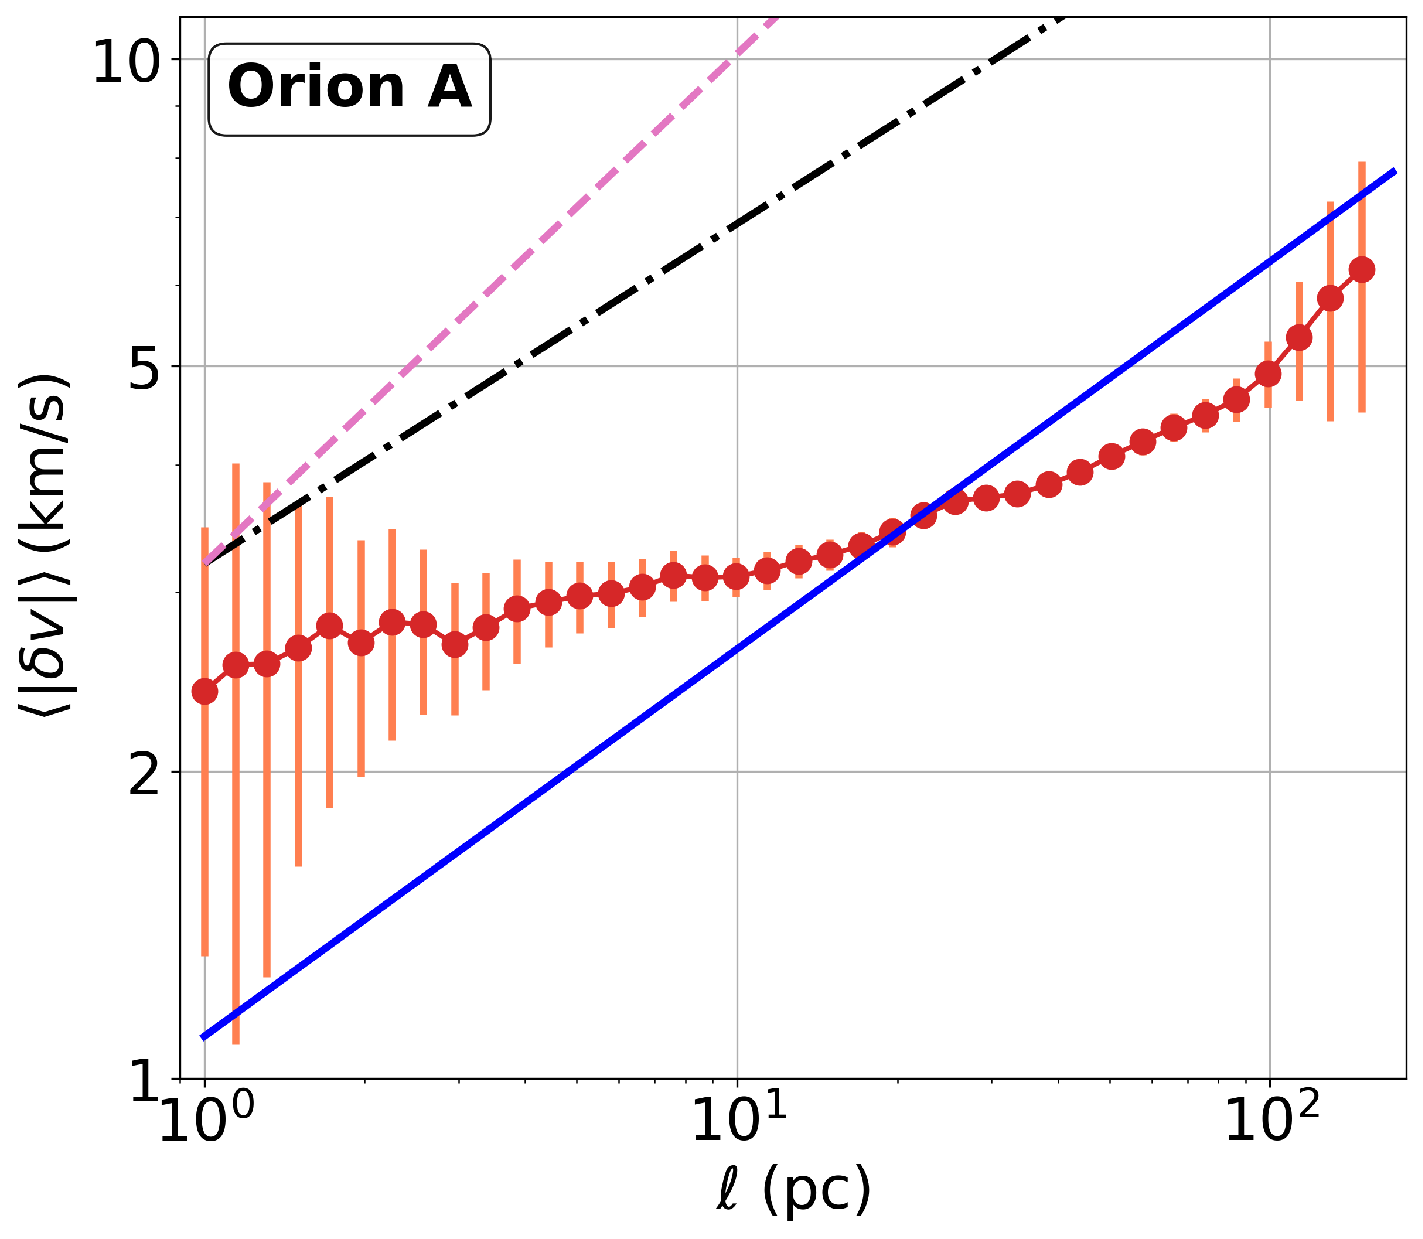
\includegraphics[width=0.32\linewidth]{Stars_img/VSF_OrionA.pdf}
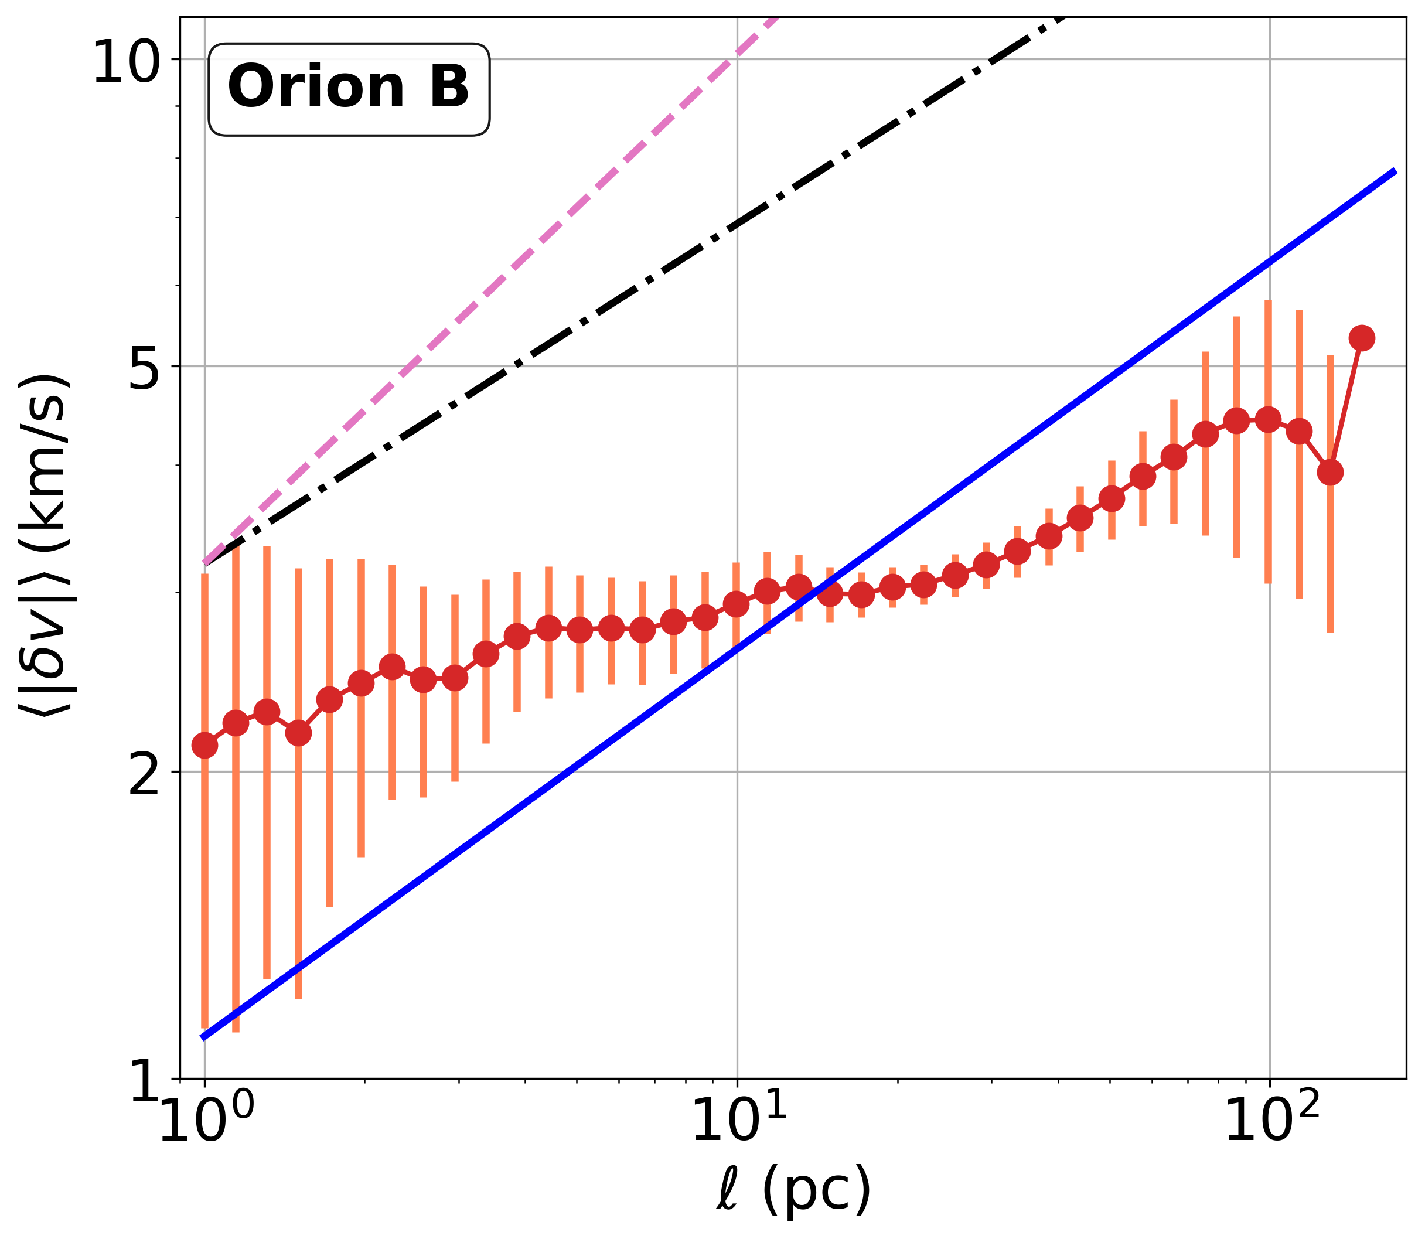
\includegraphics[width=0.32\linewidth]{Stars_img/VSF_OrionB.pdf}
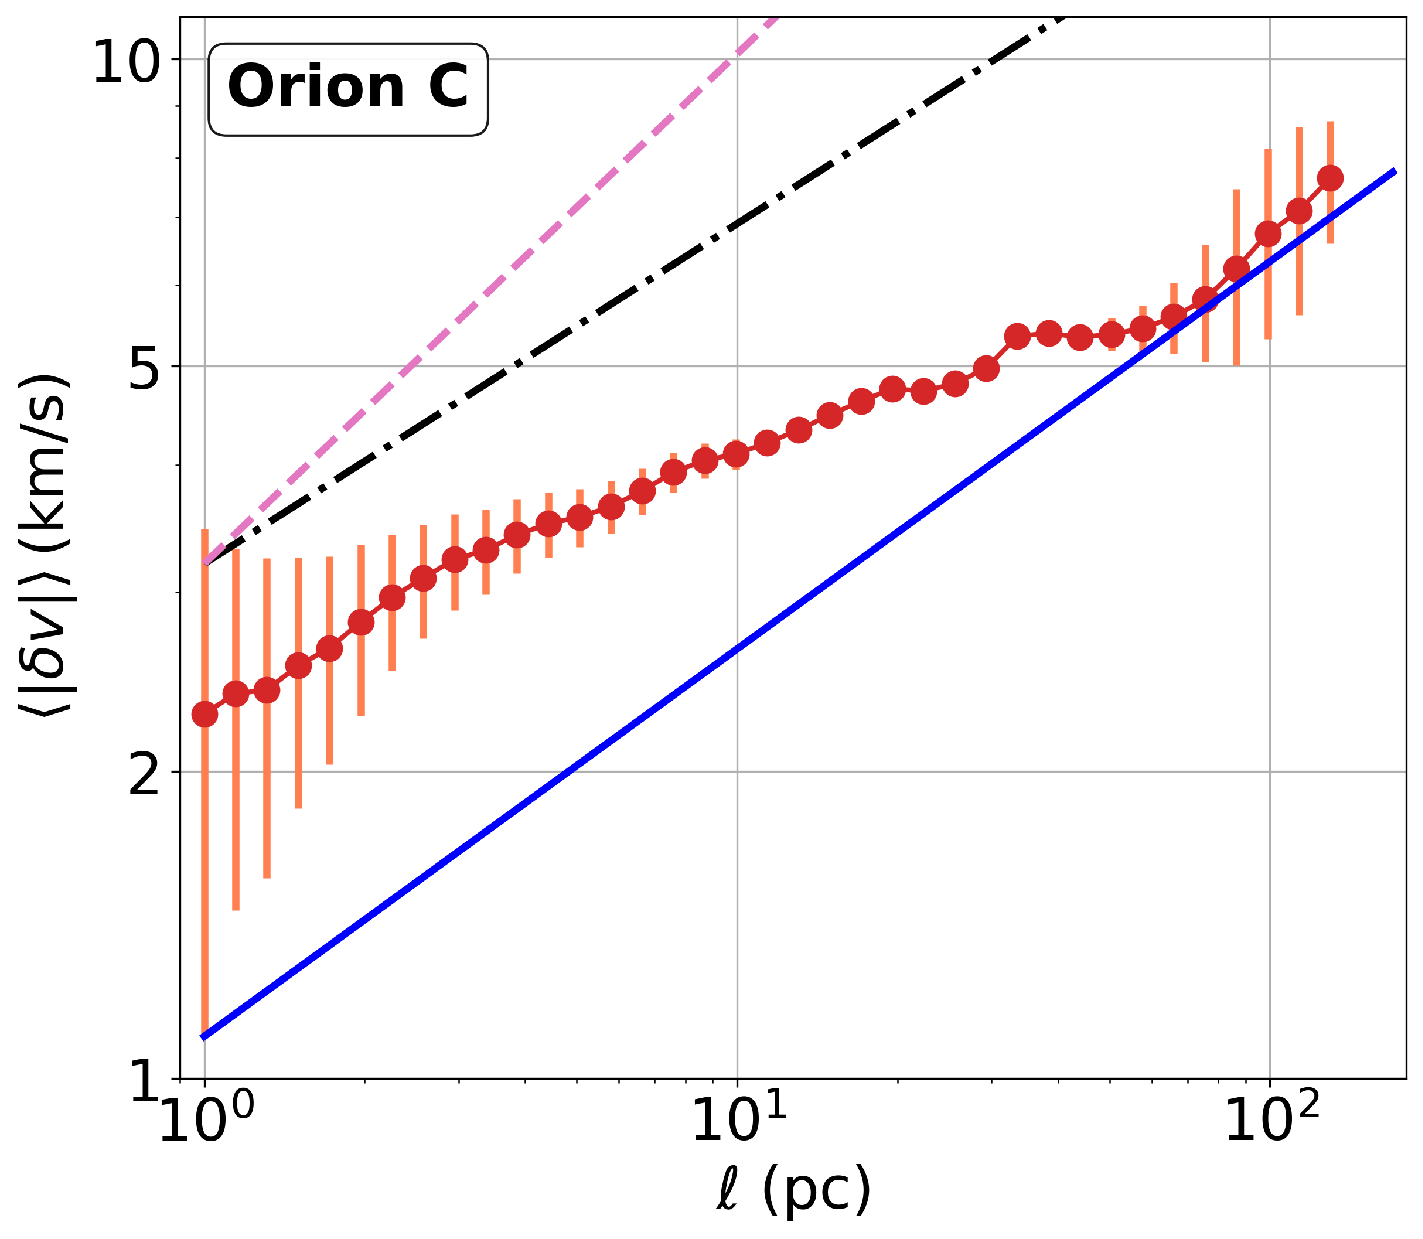
\includegraphics[width=0.32\linewidth]{Stars_img/VSF_OrionC.pdf}\\
\vskip 0.1in
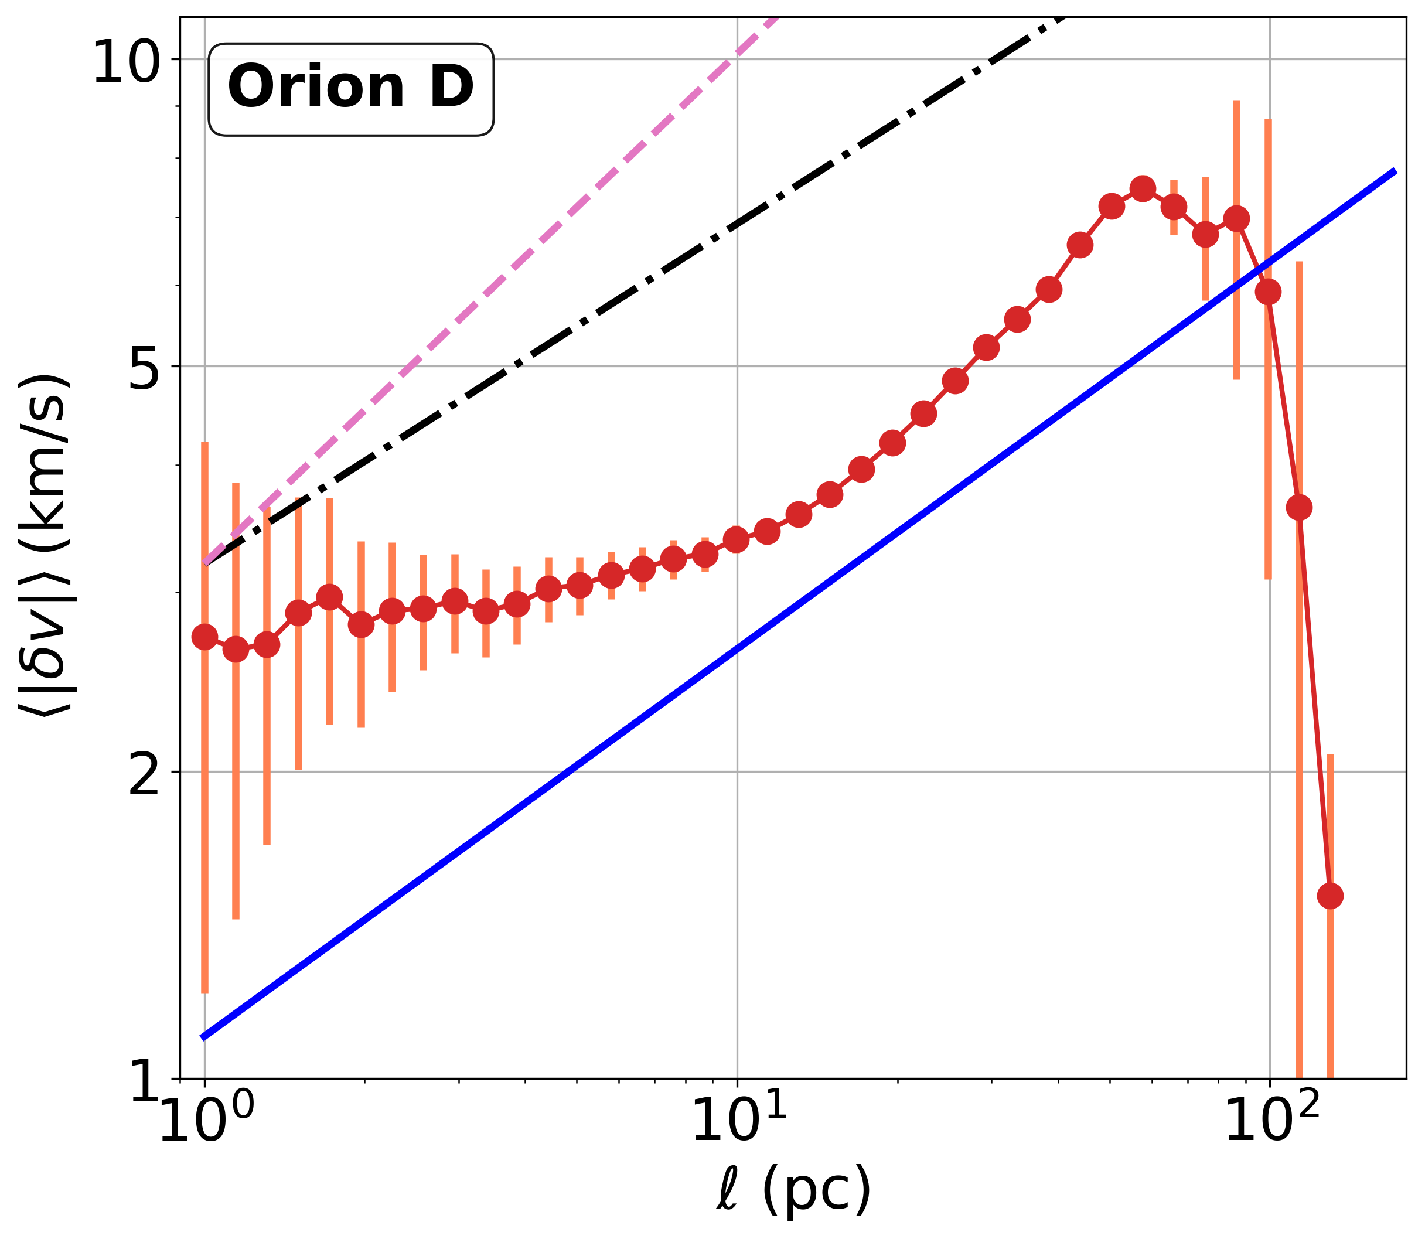
\includegraphics[width=0.32\linewidth]{Stars_img/VSF_OrionD.pdf}
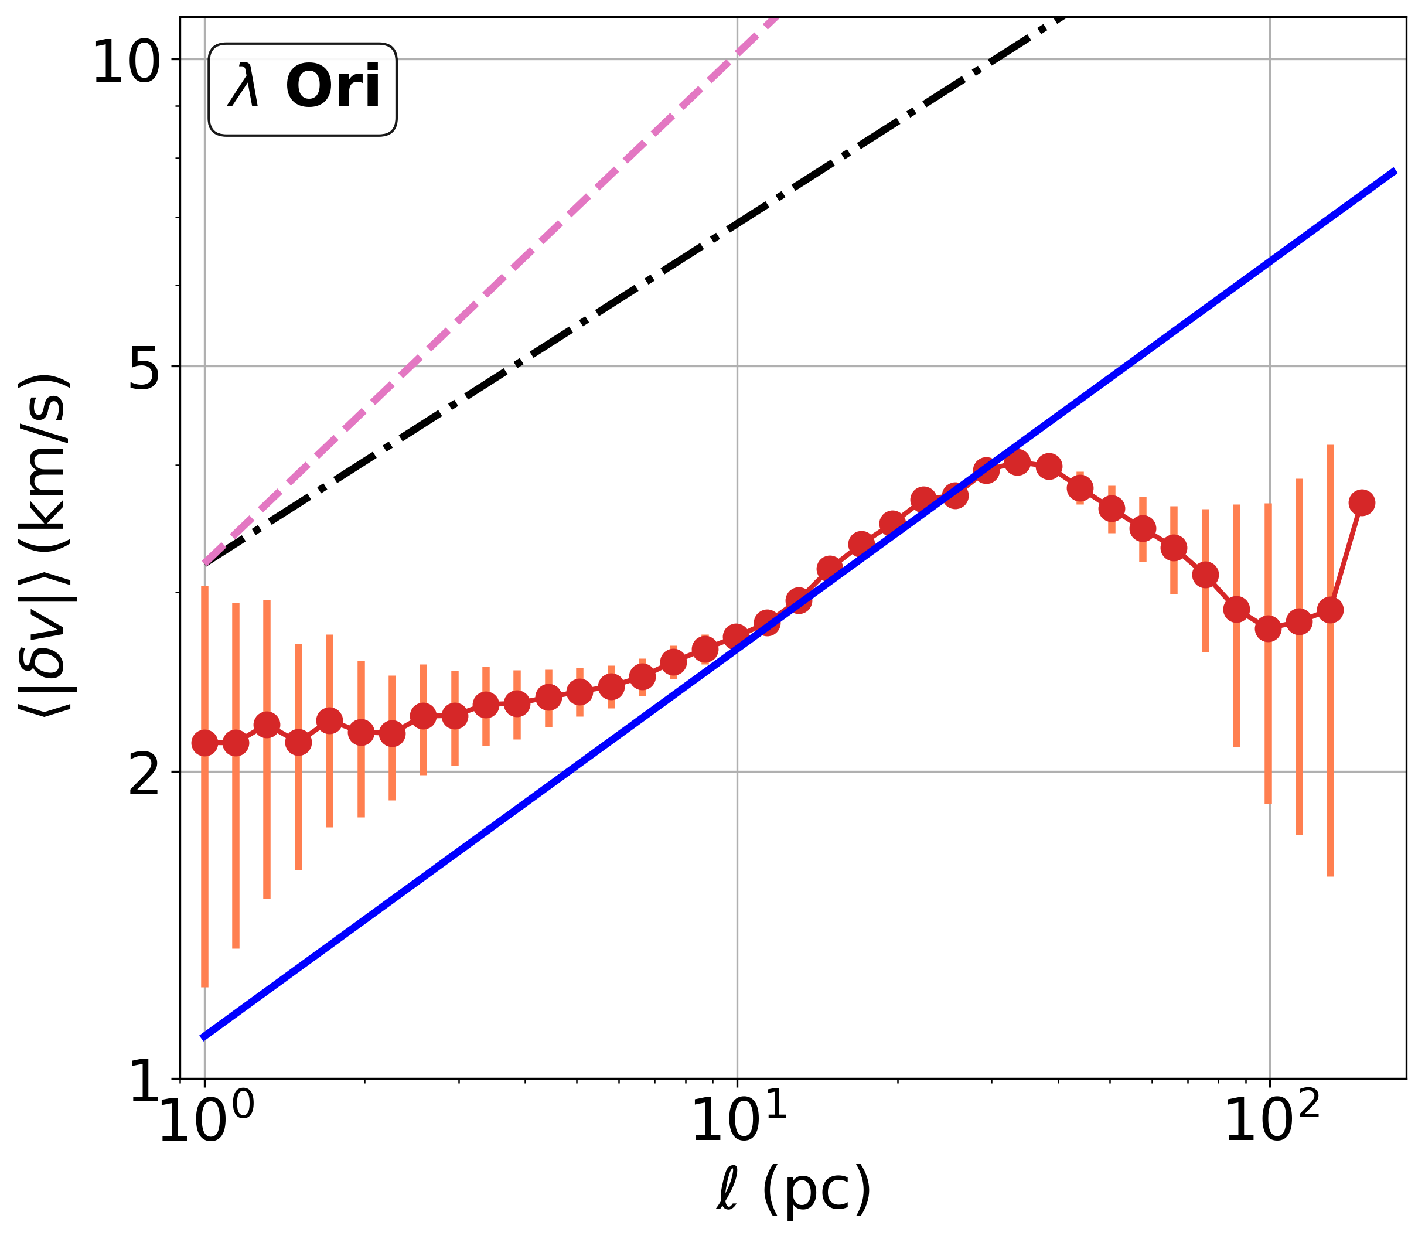
\includegraphics[width=0.32\linewidth]{Stars_img/VSF_LambdaOri.pdf}
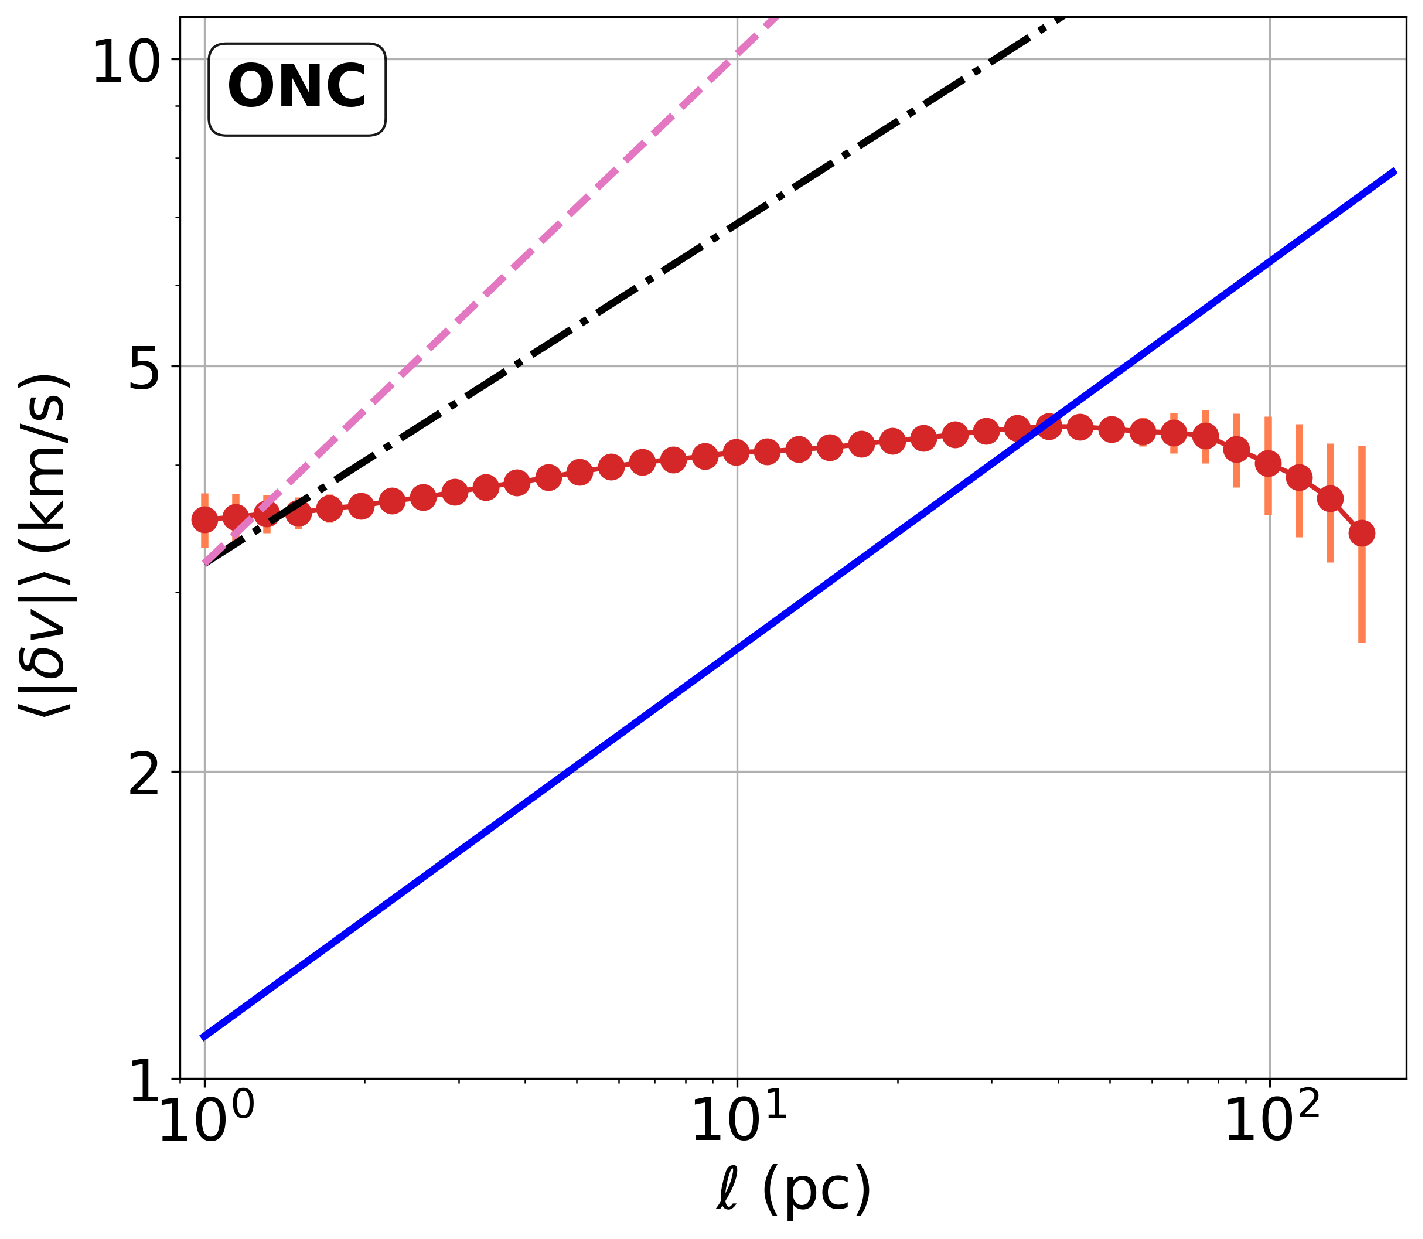
\includegraphics[width=0.32\linewidth]{Stars_img/VSF_ONC.pdf}\\
\vskip 0.1in
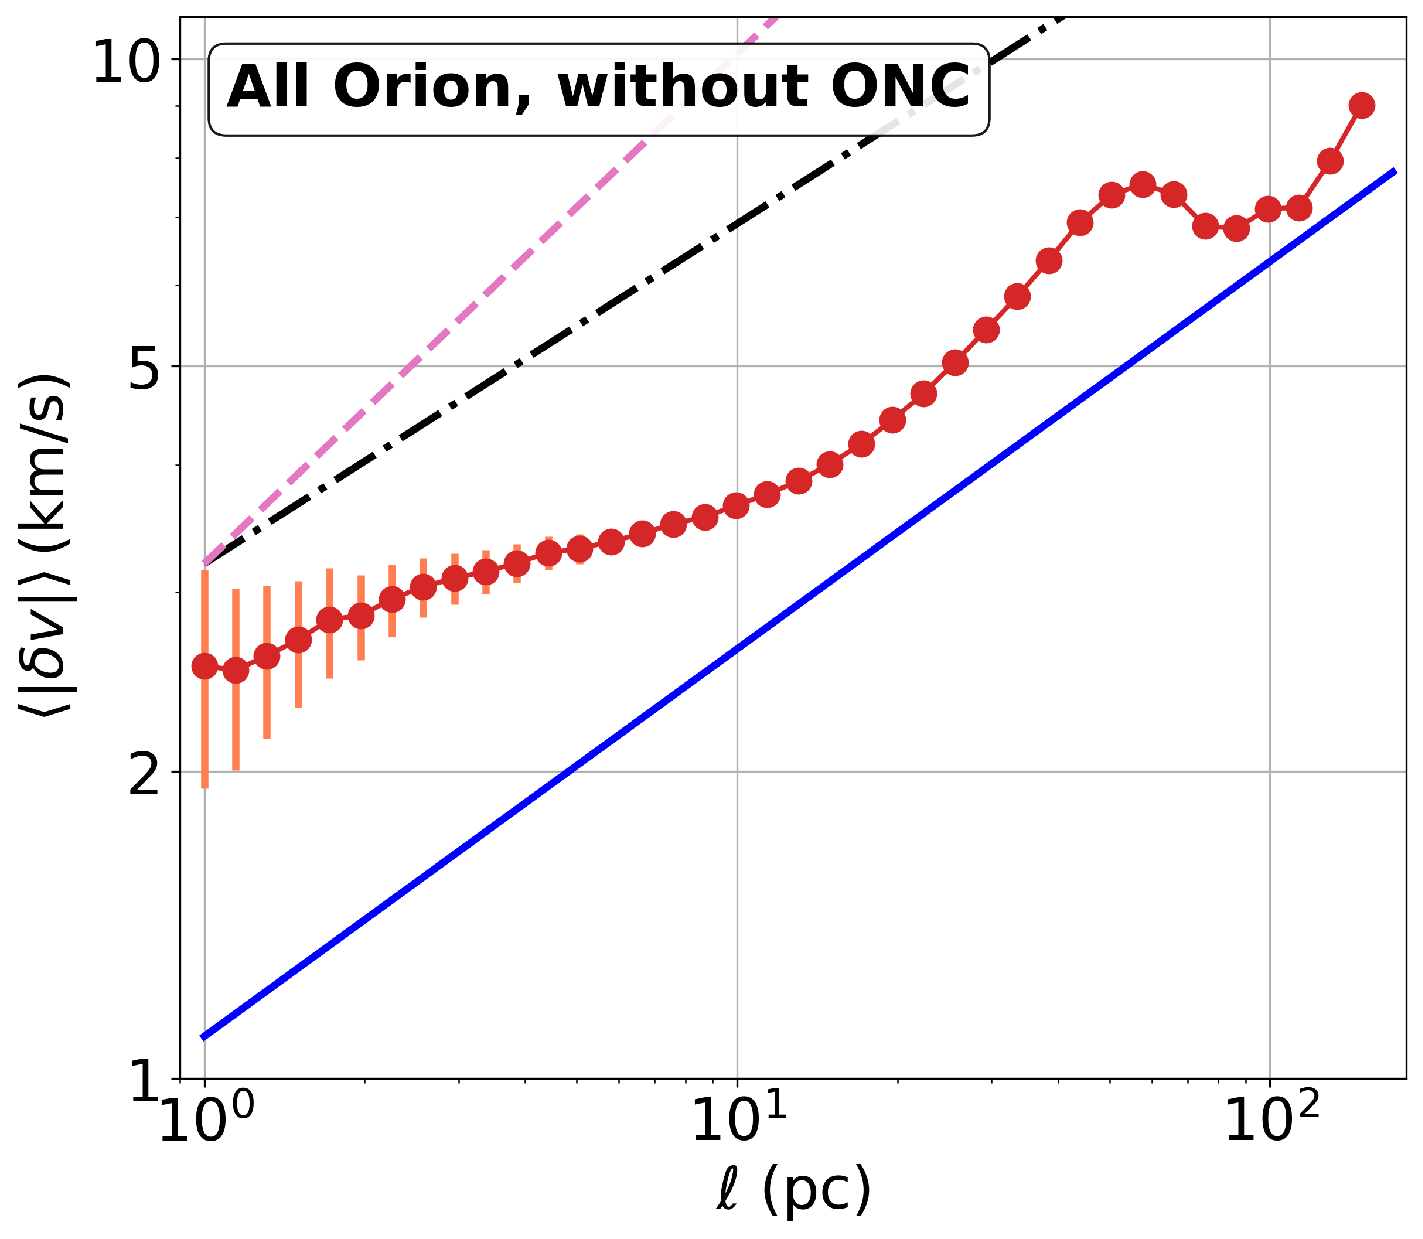
\includegraphics[width=0.32\linewidth]{Stars_img/VSF_Orion_noONC.pdf}
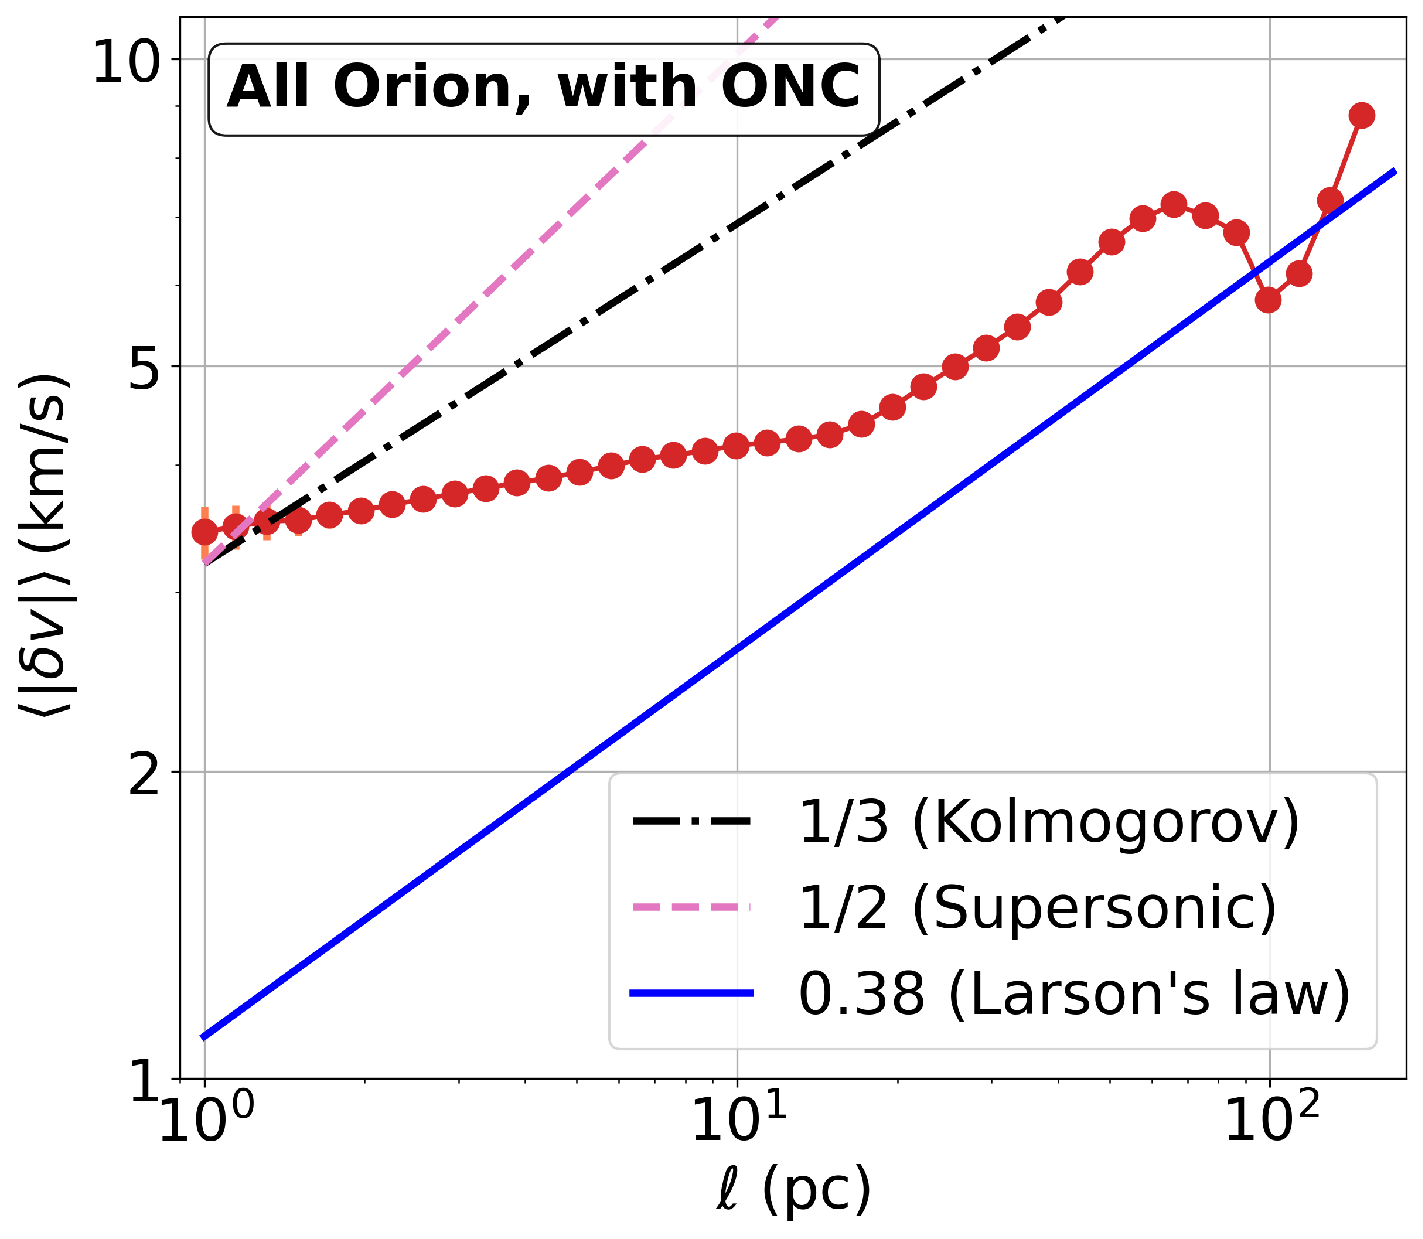
\includegraphics[width=0.32\linewidth]{Stars_img/VSF_Orion_withONC.pdf}
\caption{Left to right, top to bottom: first-order VSF of stars in the Orion A, Orion B, Orion C, Orion D, Lambda Ori, ONC, all Orion without ONC, and all Orion with ONC\@. The error bars are obtained through a random sampling analysis, and represent the uncertainties from both observational errors and uncertainties due to small sample size. As reference, we also plot a black dot-dashed line of slope 1/3 for the Kolmogorov turbulence, a pink dashed line of slope 1/2 for supersonic turbulence, and a solid blue line for Larson's velocity dispersion correlation for molecular clouds: $\sigma (km \cdot s^{-1}) = 1.1 \cdot L (pc)^{0.38} $ \citep{larson_turbulence_1981}. All panels use 40 logarithmic bins of $\ell$ from 1 pc to 170 pc. }\label{fig:vsf}
\end{figure*}

\subsection{Results}\label{sec:orion-results}

\subsubsection{The first-order VSFs}

Figure~\ref{fig:vsf} shows the first-order VSF of stars in all six individual groups in the Orion Complex. The last two panels show the combined VSF of all groups without and with the ONC, respectively. 
To guide the eye, we also plot in each panel the expected scaling for supersonic and subsonic turbulence, along with Larson's law measured for turbulence in molecular clouds in the Milky Way \citep{larson_turbulence_1981}.

The VSFs of all six individual groups except ONC exhibit a power-law scaling, characteristic of a turbulent flow. The amplitudes and slopes vary from group to group. The best-fit VSF slopes are listed in Table~\ref{table:data}.

The Orion A group (top left panel of Figure~\ref{fig:vsf}) is located just outside of Barnard's Loop (the shell-like feature to the left of Orion A-D in Figure~\ref{fig:orion}, see also \citet{ochsendorf_nested_2015}), which is proposed to have originated from a supernova that erupted $\sim$6 Myr ago \citep{kounkel_supernovae_2020}. Due to its location, Orion A is largely unaffected by the supernova's shock wave. Indeed we observe that its VSF slope generally follows that of subsonic turbulence. The overall amplitude is slightly below Larson's relation. 

The Orion B cloud is connected to Orion A but closer to the center of the supernova explosion. Our analysis of the Orion B group suffers from high uncertainties due to low number of stars (51) available in the catalog. The slope of the VSF of Orion B (top middle panel) is not well constrained, but the VSF generally follows the turbulence-like kinematics present in other clouds. The amplitude is roughly consistent with Larson's relation.

Orion C lies within the supernova bubble, and as \citet{kounkel_supernovae_2020} suggested, was driven apart from Orion D at the opposite front of the supernova shock wave. Most of the stars in Orion C and D formed after the supernova explosion that created the Barnard's Loop. We observe this local energy injection effect on the VSF of Orion C (top right panel) with a higher-than-Larson amplitude. 
The slope of the VSF is flatter than the Kolmogorov turbulence due to the presence of $\sigma$ Ori, a dense cluster of age $\sim$2 Myr. We discuss the effects of dense clusters on the VSF in more detail later in this section. 

Stars in the Orion D group exhibit a curious VSF (middle left panel), with a slope more in line with supersonic turbulence (slope $1/2$) than Kolmogorov at distance scale $10<\ell<60$ pc and absolute velocity difference higher than that of Larson's law. We attribute these properties of Orion D's VSF to its position inside the supernova bubble. Located close by and at the front of the bubble (in our line-of-sight) as it expands, motion of stars in the Orion D cloud is additionally driven by the shock wave of the supernova, hence its turbulent kinetic energy is amplified. 


The last independent group we look at is $\lambda$ Ori (center panel of Figure~\ref{fig:vsf}). In the $10<\ell<32$ pc range, the VSF of stars in $\lambda$ Ori closely exhibits the 0.38 slope of Larson's law. The amplitude also exactly follows Larson's relation \citep{larson_turbulence_1981}, and is higher than Orion A and B, but lower than Orion C and Orion D. This result can be understood given $\lambda$ Ori's history and isolated position in the Orion Complex. The $\lambda$ Orion bubble (the bubble-like structure surrounding $\lambda$ Ori in Figure~\ref{fig:orion}) is proposed to have been created by a supernova explosion $\sim1$ Myr ago \citep{dolan_photometric_2002}. Although \citet{kounkel_supernovae_2020} estimated the age of the remnant to be $\sim 4$ Myr. Regardless, the explosion happened after many of the stars have already formed in $\lambda$ Ori where the stellar age has a wide spread over $\sim 6$ Myr \citep{kounkel_apogee-2_2018}. Thus the effect of local energy injection is not as prominent as in Orion C and D.

The ONC's VSF (middle right panel) has a distinctively flatter slope compared to other groups in the Orion Complex. The ONC is a dense star cluster located at one end of the Orion A molecular cloud (Figure~\ref{fig:orion}). Unlike the loose star groups discussed previously, the ONC has a dense inner core ($\sim 2$ pc) with an estimated relaxation time of $\tau_r \sim$ 0.6 Myr \citep{hillenbrand_preliminary_1998}, shorter than the cluster's mean age of $\sim$ 2.6 Myr. Therefore, a significant fraction of the stars in the ONC have dynamically relaxed, and have hence ``forgotten" the turbulence kinematics of their natal clouds. The residual non-zero slope likely originates from the stars in the outer parts of the cluster that have not relaxed yet. It is worth noting that if we simply look at the velocity distributions of stars in different groups (Figure~\ref{fig:velodist}), ONC does not appear drastically different from the rest of the groups apart from its compactness in the velocity space. Yet our analysis reveals its distinct kinematics due to relaxation.

In the last two panels of Figure~\ref{fig:vsf}, we compute the VSF for all the stars within the Orion Complex without and with the ONC (bottom left and bottom right panels, respectively). Without the ONC, the VSF of the Orion Complex has similar characteristics to that of Orion D, with a steeper-than-Kolmogorov slope and an amplitude higher than Larson's law in the $10<\ell<60$ pc scale range. This is because D has the highest number of stars amongst the 5 groups (Table ~\ref{table:data}). 

When the ONC is included, on small scales ($2<\ell<20$ pc), the VSF flattens because it is heavily influenced by the cluster due to its dominant number of stars in the catalog (585 stars vs. a total of 1439 stars). In fact, this is why we separate the ONC from Orion A in our analysis. If we include ONC in Orion A, the resulting VSF is significantly flatter. All the other star groups also contain star clusters. For example, Orion C has $\sigma$ Ori. We do not separate these clusters because they are much smaller than the ONC, and removing them degrades the statistics of our analysis. We note, however, that they may have contributed to the flatter VSF of Orion C and the flattening of the VSF in the other groups on small scales. We discuss other uncertainties in more detail in Section~\ref{sec:discussions}. 

The combined VSF shows a bump at $\sim 60$ pc, similar to Orion D, suggesting energy injection at that scale. The mean age of the stars in this study is $\sim 3.7$ Myr. Given the current size of the Barnard's loop ($\sim 80$ pc) and its age ($\sim 6$ Myr), the energy injection scale is roughly consistent with the size of the supernova bubble when the stars first formed. This again shows the effects of local energy injection of supernova explosions on turbulence.



\subsection{Discussions}\label{sec:discussions}

\subsubsection{Biases and Uncertainties}

Gas in molecular clouds such as the Orion Complex is turbulent by nature. The theoretical foundation of our analysis is that newborn stars retain this turbulence information. However, after the stars are born, they decouple from the hydro-dynamical forces of the gas, and no longer follow the turbulent flow. In other words, stars are only perfect tracers of turbulence at birth. Since star formation happens over a period of time, all of the star groups contain stars that are over a few Myr old. We have identified two mechanisms through which stars can lose their memory of the ISM turbulence, causing biases in our analysis.

The first mechanism is dynamical relaxation, which we discussed in the analysis of the ONC in Section~\ref{sec:orion-results}. Due to open clusters' high density, close stellar encounters are common, which alter the stars' original orbits and lead to dynamical relaxation. The relaxation time is estimated as a function of the number of stars and the crossing time of the cluster:

\begin{equation}
t_{relax} = t_{cross} \cdot \frac{N}{6 \cdot \ln{N/2}} \,,
\end{equation}
where $N$ is the total number of stars in the cluster and $t_{cross}$ is the crossing time, defined as the typical time for a star to travel a distance equal to the half-mass size of the cluster:

\begin{equation}
t_{cross} =  \frac{2 \cdot R_{hm}}{\sigma_v} \,.
\end{equation}
Here, $R_{hm}$ is the radius within which half of the cluster's stars reside, and $\sigma_v$ is the bulk-motion-removed characteristic velocity of the cluster's stars. It is computed as the standard deviation of the velocity distribution with respect to the median \(\sigma_v \equiv \sigma [|v_i - v_{median}|]\).

After the stars are relaxed, they no longer hold the turbulent kinematics of gas at the time of their formation. For loose groups of stars such as those we analyze, the crossing times are significantly longer than the group's current age (Table~\ref{table:data}). Furthermore, since each group possesses a number of stars in the order of N $\sim 10^3$ (e.g., N = 2800 stars within the dense core of the ONC was used by \citet{hillenbrand_preliminary_1998}), the estimated relaxation time is an order of magnitude longer than the crossing time. Therefore, dynamical relaxation has most likely not affected the shape of the VSF for the five groups in the Orion Complex, except for the ONC\@. This is in agreement with \citet{da_rio_-sync_2017} who find that young stars in Orion A are kinematically associated with the molecular gas, but the ONC appears more dynamically evolved and virialized. \citet{kounkel_apogee-2_2018} also found consistent kinematics between young stars and gas in the whole Orion Complex where the gas has not been dispersed.

In addition to the ONC, there are other clusters within each group: $\sigma$ Ori in Orion C, 25 Ori in Orion D, $\lambda$ Orionis Cluster in $\lambda$ Ori, and two small clusters NGC 2024 and NGC 2068 in the Orion B group. These clusters have much smaller physical sizes than the ONC and contain only a small fraction of stars of the group. This property of the clusters can be visually confirmed from Figure~\ref{fig:orion}. Thus, their existence does not significantly affect our overall results. However, they may have contributed to the flattening of the VSFs on small scales that we observe in almost all individual groups.

Another potential source of bias in our analysis comes simply from the drifting of stars from their original positions. Assuming no strong stellar encounters, stars with higher velocity differences drift apart at a faster rate than stars with smaller velocity differences, causing the VSF to steepen with time. This steepening happens over roughly $t_{cross}$.

In our analysis, most groups are relatively young, with their ages much shorter than $t_{cross}$ (Table~\ref{table:data}), so drifting should not have had time to erase turbulence-driven velocity differences. Although drifting may have steepened the VSF of Orion D, which has the oldest median age and the steepest slope amongst all the groups analyzed here. We plan to further explore the effects of relaxation and drifting in our future works both with a larger observed sample and with numerical simulations \citep{li_disruption_2019}. 

There are also other sources of uncertainties in our analysis, such as binary systems. While the barycenter should follow the turbulent velocity of the natal cloud, binaries also have orbital motion contributing to the overall velocity measurement. While most systems with very large orbital speeds have been excluded from the analysis through the initial hierarchical clustering, systems with orbital speeds of only a few km s$^{-1}$ likely remain.

False positives in hierarchical clustering, such as contamination from the field stars, can also affect our results. \citet{kounkel_apogee-2_2018} estimated that false positive fraction for the clustering algorithm can be as high as $\sim$6\%. In addition, drifting can result in close pairs of uncorrelated stars with high relative velocity. Binaries, drifting, and mis-grouped stars, coupled with small sample sizes at small separations would explain the flattening of the VSFs at small $\ell$.

\subsubsection{Comparison with other Methods to Measure Turbulence}
Most of the previous studies on turbulence in astrophysical environments rely on the observations of gas. Although only velocity statistics can directly 
reflect the dynamics of turbulence and turbulent energy cascade, 
it is the density statistics that is widely used for measuring turbulence as it is much more easily accessible to observations. For example, the delta-variance method has been used to analyze the structure of observed molecular cloud images in the ISM \citep{stutzki_fractal_1998}. The same method and a modification of it \citep{arevalo_mexican_2012} have also been used to infer turbulence in the hot intracluster medium based on X-ray images \citep[e.g.,][]{zhuravleva_turbulent_2014}.%

Velocity centroids can recover the turbulent velocity spectra in subsonic turbulence 
\citep{esquivel_velocity_2005}. 
The velocity channel analysis (VCA)
using channel maps and 
velocity coordinate spectrum (VCS)
using the fluctuations 
measured along the velocity axis of the Position--Position--Velocity (PPV) cubes
can also be used to extract turbulent velocity spectra in supersonic turbulence
(see \cite{lazarian_obtaining_2009} for a review). 
In particular, the VCS technique only requires measurements along a few directions to obtain a reliable velocity spectrum
\citep{chepurnov_turbulence_2009}. Spectroscopic data has also been used in the Principal Component Analysis to extract the size-line width relation and recover the structure function within molecular clouds, as reported by \citet{heyer_universality_2004} and \citet{roman-duval_turbulence_2011}.

Recently, statistical measurements of the velocities of gas phase point sources have been developed for, e.g., dense molecular cores embedded in the background turbulent flow \citep{qian_13co_2012} and filaments in the centers of galaxy clusters \citep{li_direct_2020}. These analyses use the 1D line-of-sight velocities and 2D positions projected on the plane of the sky. The bias due to the projection effect depends on the thickness of the structure \citep{qian_new_2015}, which is usually unknown.

Our analysis in spirit is similar to that of gas phase point sources, but instead of using projected information, we take advantage of the full 6D (3D velocity + 3D position) information of stars. Thus our results do not suffer from the poorly constrained projection uncertainties. Observing 6D information of the gas, especially the motions in the plane of the sky, is prohibitively challenging \citep[although see][]{odell_high_2008}. Thus our method has a unique advantage, and can potentially be used to help better understand the biases in the analyses based on gas.


\subsubsection{Comparison with Theories and Other Observations}

There has been a lot of previous work on turbulence in Orion based on the observations of emission lines of the ionized gas \citep{castaneda_velocity_1988, odell_motion_1992, mcleod_nebular_2016, arthur_turbulence_2016}. Most of them are focused on small scales ($<1$ pc) and therefore cannot be directly compared with our results. But they do generally find VSFs consistent with turbulence, in agreement with our results.

On larger scales (a few to $\sim 100$ pc), we have compared our results with Larson's Law in Section~\ref{sec:orion-results}. Individual groups may show slightly higher or lower amplitude than the mean Larson's relation, with slightly steeper or shallower slopes, but overall, our results are in good agreement with Larson's Law for molecular clouds in the Milky Way. Notably, \citet{larson_turbulence_1981} also finds a slightly lower-than-average amplitude for Orion B, consistent with our findings here even though we are using different tracers of turbulence. 

Our results show that regions heavily influenced by supernova explosions can exhibit a higher level of turbulence, and even a steeper VSF\@. This is consistent with numerical simulations showing that supernovae can drive turbulence in molecular clouds \citep{padoan_supernova_2016}.
Additionally, the steepened slope of Orion D is consistent with \citet{federrath_universality_2013} finding that supernova explosions excite more compressible than solenoidal velocity modes in the gas, which tends to steepen the VSFs, and thus exhibit the 1/2 power law of supersonic turbulence. Observations have also shown the local effects of supernovae on turbulence in other systems (e.g., in the Large Magellanic Clouds \citep{szotkowski_mapping_2019}). 

\subsection{Concluding Remarks and Future Work}
We have introduced a new method to study turbulence in the ISM using motions of 
young stars. Our results demonstrate that stars in young star groups retain the memory of turbulence of their natal molecular clouds. Our analysis uses the full 6D information of stars to trace turbulence, and does not suffer from projection uncertainties. Our results can be used to provide independent constraints on the turbulent properties of molecular clouds in addition to analysis of gas kinematics, and also shed light on studies of the dynamical evolution of star clusters in the Galaxy \citep{kamdar_dynamical_2019}. 

We plan to apply our analysis to a much larger sample of star groups in the future. Meanwhile, we will perform and analyze tailored numerical simulations of star formation in molecular clouds to better understand biases and uncertainties in our analysis, as well as constraining subgrid models for star formation \citep{li_disruption_2019}. 

\subsection{Supplemental Material}

\subsubsection{The higher-order VSFs}
\label{subsec:high_order}

We present the second and third order VSFs in Figure~\ref{fig:3rdorder}.
High order VSFs are usually used to evaluate the intermittency
\citep{she_universal_1994,boldyrev_supersonic_2002}.
Different behaviors of the high-order VSFs measured with different gas tracers, e.g., $H_2$, $CO$, were found in numerical simulations of molecular clouds,
which are related to their different volume filling factors and spatial distribution
\citep{bertram_centroid_2015}.
The second and third order VSFs that we present in Figure~\ref{fig:3rdorder}
are generally consistent with the Kolmogorov scaling. This finding agrees with the
measurement using the velocities of dense cores in Taurus cloud
\citep{qian_studies_2018}.
It suggests that both the dense cores and the stars used here sample the turbulence in the relatively diffuse region with a large volume filling factor, and thus the Kolmogorov scaling is expected \citep{xu_projected_2020}.

\label{sec:2ndvsf}
\begin{figure}
    \centering
    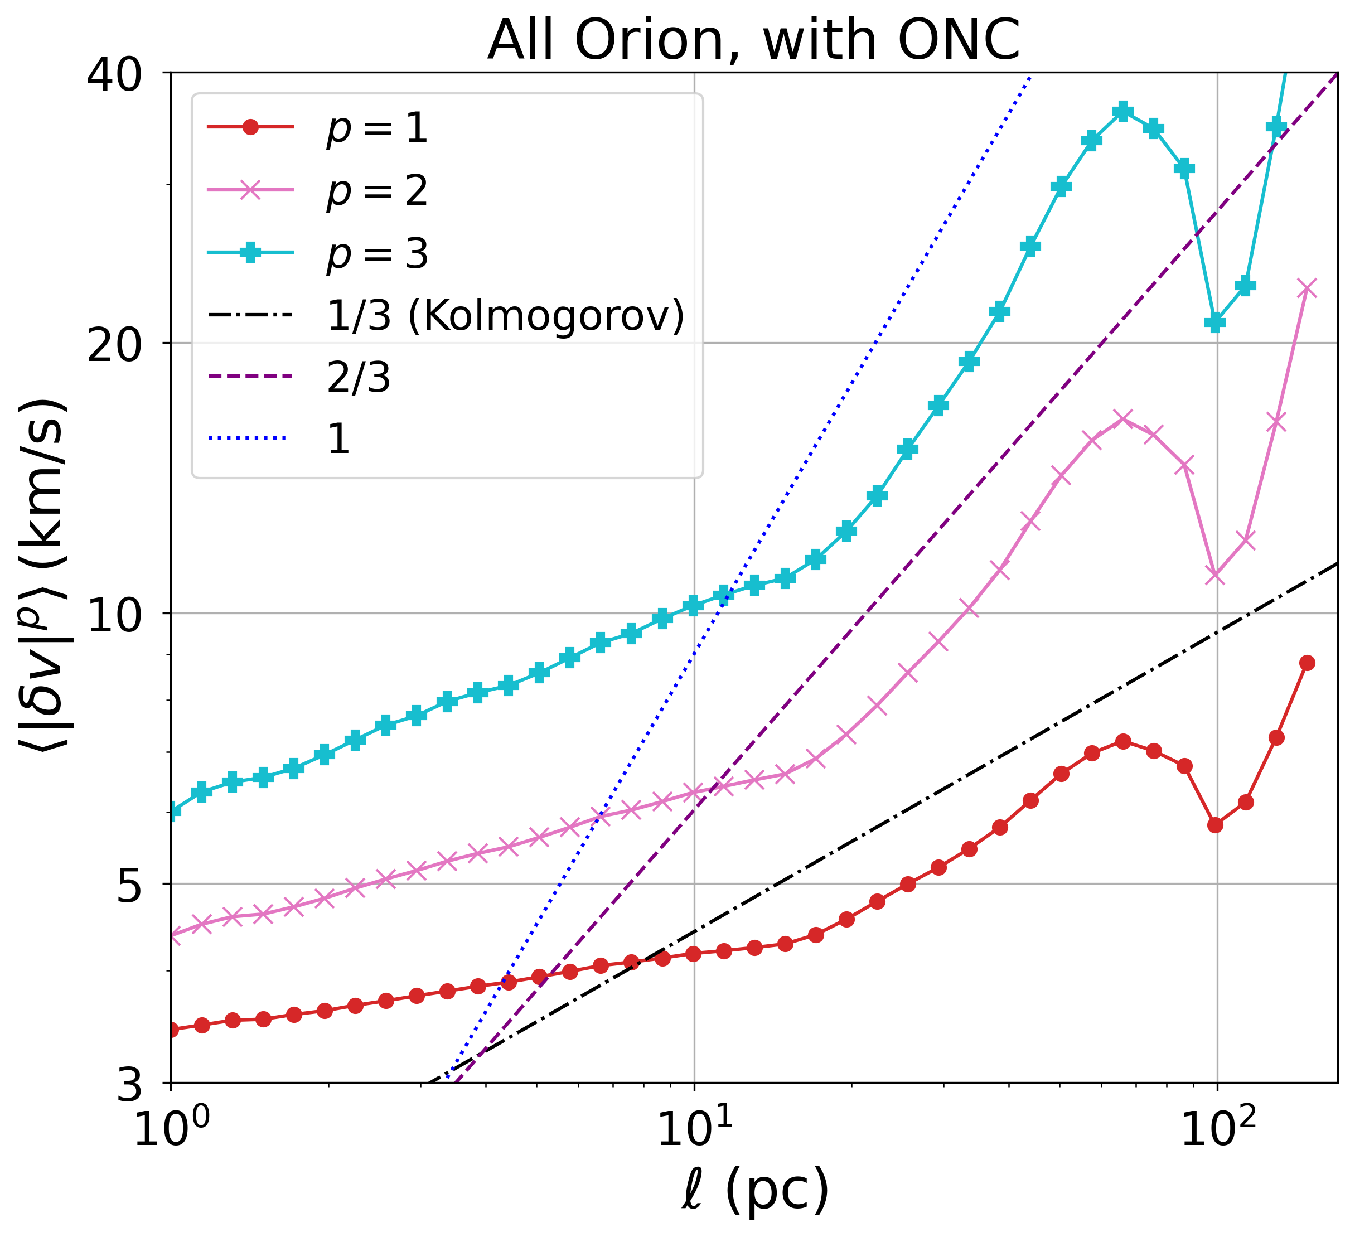
\includegraphics[width=0.7\linewidth]{Stars_img/3rdorder_Orion.pdf}
    \caption{First ($p=1$, red), second ($p=2$, pink), and third ($p=3$, blue) order VSFs of the stars in the entire Orion Complex. The second and third order VSFs have been shifted lower for easy comparison.}
    \label{fig:3rdorder}
\end{figure}


\section{Ophiuchus, Perseus, Taurus, and Comparing Stellar Motion Against Gas}

\publicationdetails
{Ha et al. 2022, ApJ, 934, 7}
{Trung Ha\footnotemark[1], Yuan Li\footnotemark[1], Marina Kounkel\footnotemark[2], Siyao Xu\footnotemark[3]\footnotemark[4], Hui Li\footnotemark[5]\footnotemark[4], and Yong Zheng\footnotemark[6]}
{The interstellar medium (ISM) is turbulent over vast scales and in various phases. In this paper, we study turbulence with different tracers in four nearby star-forming regions: Orion, Ophiuchus, Perseus, and Taurus. We combine the APOGEE-2 and Gaia surveys to obtain the full six-dimensional measurements of positions and velocities of young stars in these regions. The velocity structure functions (VSFs) of the stars show a universal scaling of turbulence. We also obtain \halpha~gas kinematics in these four regions from the Wisconsin H-Alpha Mapper. The VSFs of the \halpha~are more diverse compared to those of stars. In regions with recent supernova activities, they show characteristics of local energy injections and higher amplitudes compared to the VSFs of stars and of CO from the literature. Such difference in amplitude of the VSFs can be explained by the different energy and momentum transport from supernovae into different phases of the ISM, thus resulting in higher levels of turbulence in the warm ionized phase traced by \halpha. In regions without recent supernova activities, the VSFs of young stars, \halpha, and CO are generally consistent, indicating well-coupled turbulence between different phases. Within individual regions, the brighter parts of the \halpha~gas tend to have a higher level of turbulence than the low-emission parts. Our findings support a complex picture of the Milky Way ISM, where turbulence can be driven at different scales and inject energy unevenly into different phases.}
{\footnotetext[1]{Department of Physics, University of North Texas, Denton, TX 76203, USA}
\footnotetext[2]{Physics \& Astronomy Department, Vanderbilt University, PMB 401807, 2301 Vanderbilt Place, Nashville, TN 37235, USA}
\footnotetext[3]{Institute for Advanced Study, 1 Einstein Drive, Princeton, NJ 08540, USA}
\footnotetext[4]{NASA Hubble Fellow}
\footnotetext[5]{Department of Astronomy, Columbia University, 550 West 120th Street, New York, NY 10027, USA}
\footnotetext[6]{Department of Astronomy, University of California, Berkeley, CA 94720, USA}}
\setcounter{footnote}{0}

\subsection{Introduction} \label{sec:multi-region-intro}

The interstellar medium (ISM) is multiphase and turbulent. Interstellar turbulence affects the velocity statistics on all scales from the diffuse ionized gas to the dense molecular gas. \citet{larson_turbulence_1981} compiled the internal velocity dispersion of nearby molecular clouds from the width of various emission lines, and found a power-law relation between the velocity dispersion and cloud size, with slope 0.38, between the 1/3 slope expected for turbulence dominated by solenoidal motions \citep{kolmogorov_local_1941} and the 1/2 slope expected for shock-dominated turbulence \citep[e.g.,][]{galtier_exact_2011,federrath_universality_2013}.

Inside molecular clouds, massive O- and B-type stars create \ion{H}{2} regions by ionizing and heating the ISM with UV radiation \citep[see, e.g.,][]{spitzer_physical_1978}. 
Compression from supernova (SN) explosions can trigger further star formation \citep[][]{kennicutt_star_2012}. Interstellar processes such as SNe, stellar winds, ionizing radiation, and cosmic rays all play a role in maintaining the structure of the ISM, as well as in regulating star formation \citep[][]{hennebelle_turbulent_2012,rathjen_silcc_2021,xu_cosmic_2022,hu_velocity_2022}. Of these mechanisms, SN explosions are perhaps the most significant source of energy injection into the local ISM \citep[][]{mac_low_control_2004,padoan_supernova_2016}. 

Many numerical simulations have been carried out to study how SN explosions affect the surrounding ISM and star formation in the last decade. In general, they find that most of the kinetic energy from an SN explosion is transferred to the low-density region of the ISM in both single- \citep[see, e.g.,][]{kim_momentum_2015,martizzi_supernova_2015,li_supernova_2015} and multiple-SN events \citep[][]{padoan_supernova_2016}, suggesting that turbulence may not be evenly driven in different phases of the ISM.

Observational studies of ISM turbulence have been done with various gas tracers. 
Measurements of turbulence through density spectrum were carried out using the Wisconsin H-Alpha Mapper \citep[WHAM;][]{haffner_wisconsin_2003,haffner_early_2010}, which revealed a turbulent cascade consistent with Kolmogorov theory \citep[][]{chepurnov_velocity_2010}. \citet[][]{burkhart_characterizing_2009} found that most of the \ion{H}{1} in the Small Magellanic Cloud (SMC) is subsonic or transonic, and concluded that turbulence in the SMC is dominated by hydrodynamical pressure over magnetic pressure. 

Statistical measurements of velocity fluctuations in the neutral ISM can be done using the Velocity Channel Analysis, the Velocity Coordinate Spectrum \citep{lazarian_velocity_2000,lazarian_studying_2006}, the Delta-variance technique \citep{stutzki_fractal_1998,ossenkopf_turbulent_2002}, or the Principal Component Analysis \citep{heyer_universality_2004,roman-duval_turbulence_2011} based on spectroscopic data. These analyses generally reveal power-law spectra of turbulent velocities \citep{lazarian_obtaining_2009,chepurnov_velocity_2010}.

Additionally, kinematics of Galactic \ion{H}{2} regions have been studied using the observations of ionized gas. Fabry-Perot interferometry was used to probe the \halpha~line in emission nebulae. \citet[][]{louise_turbulence_1970} found a velocity-size relation that agrees with the 1/3 slope of Kolmogorov turbulence in M8, while \citet{roy_structure_1985} and \citet[][]{joncas_h_1986} found slopes of the structure functions closer to 1/2, indicating turbulence in the supersonic regime in both S142 and M17, respectively. 

Closer to our solar neighborhood, studies into the nature of turbulence in the Orion Nebula is an ongoing effort since the 1950s. \citet{von_hoerner_methode_1951} observed a root-mean-square difference in emission line velocities that increases with larger angular separations. He reasoned that such relation could be explained by the Kolmogorov theory if the effective depth of the nebula was sufficiently small as to neglect projection effects. Subsequent studies, carried out by \citet{munch_internal_1958} and \citet{castaneda_velocity_1988}, dispute this conclusion. \citet[][]{munch_internal_1958} found an optical depth smaller than the value postulated by \citet[][]{von_hoerner_methode_1951}, and attributed the failure of Kolmogorov theory to the compressibility of turbulence in the Orion Nebula, while \citet[][]{castaneda_velocity_1988} argued against a simple power-law relation, instead suggesting energy injections at different scales. 

ISM turbulence has also been probed using ``point sources'' such as molecular cores. \citet{qian_13co_2012} developed statistical measurements of core-to-core velocity dispersion over a range of length scales, i.e., the core velocity dispersion technique. \citet{qian_studies_2018} find signatures for a turbulent power-law spectrum in the Taurus Molecular Cloud and demonstrate that the statistics of turbulent velocities are imprinted in the velocities of dense cores \citep{xu_projected_2020}. 

One limitation of using gas tracers is they lack three-dimensional information on the position and the velocity information is also limited to only the line-of-sight.
In \citet[][hereafter Paper I]{ha_measuring_2021}, we proposed a new method to measure turbulence in the ISM with young stars. Since stars are formed out of turbulent molecular clouds, we expected these young stars to inherit the turbulent kinematics from their natal clouds. Using six-dimensional position and velocity information of $> 1400$~stars in the Orion Complex, we found that the first-order velocity structure function (VSF) of young stars in loose groups exhibit characteristics of turbulence. Our method can therefore be used to probe the turbulent properties of molecular clouds in addition to analysis of gas kinematics and has been used in recent work in \citet{krolikowski_gaia_2021,zhou_kinematics_2022}. 

In this work, we apply a similar analysis to a larger sample of molecular complexes, which include three of the nearest massive star-forming regions: Ophiuchus, Perseus, and Taurus. Additionally, we analyze the kinematics of \halpha~gas from the WHAM survey to study the connection between stars and the multiphase ISM.

In Section \ref{sec:data_method}, we describe the data used in this analysis, the reduction pipeline for the \halpha~kinematic survey, and how we compute the VSFs using stars and \halpha. In Section \ref{sec:multi-region-results}, we present the VSF of young stars and multiphase gas of all four regions.
In Section \ref{sec:multi-region-discussion}, we discuss sources of uncertainty associated with our analysis and the nature of turbulence in the Milky Way ISM\@. We summarize our results in Section \ref{sec:conclusions}.


\begin{figure*}
    \centering
    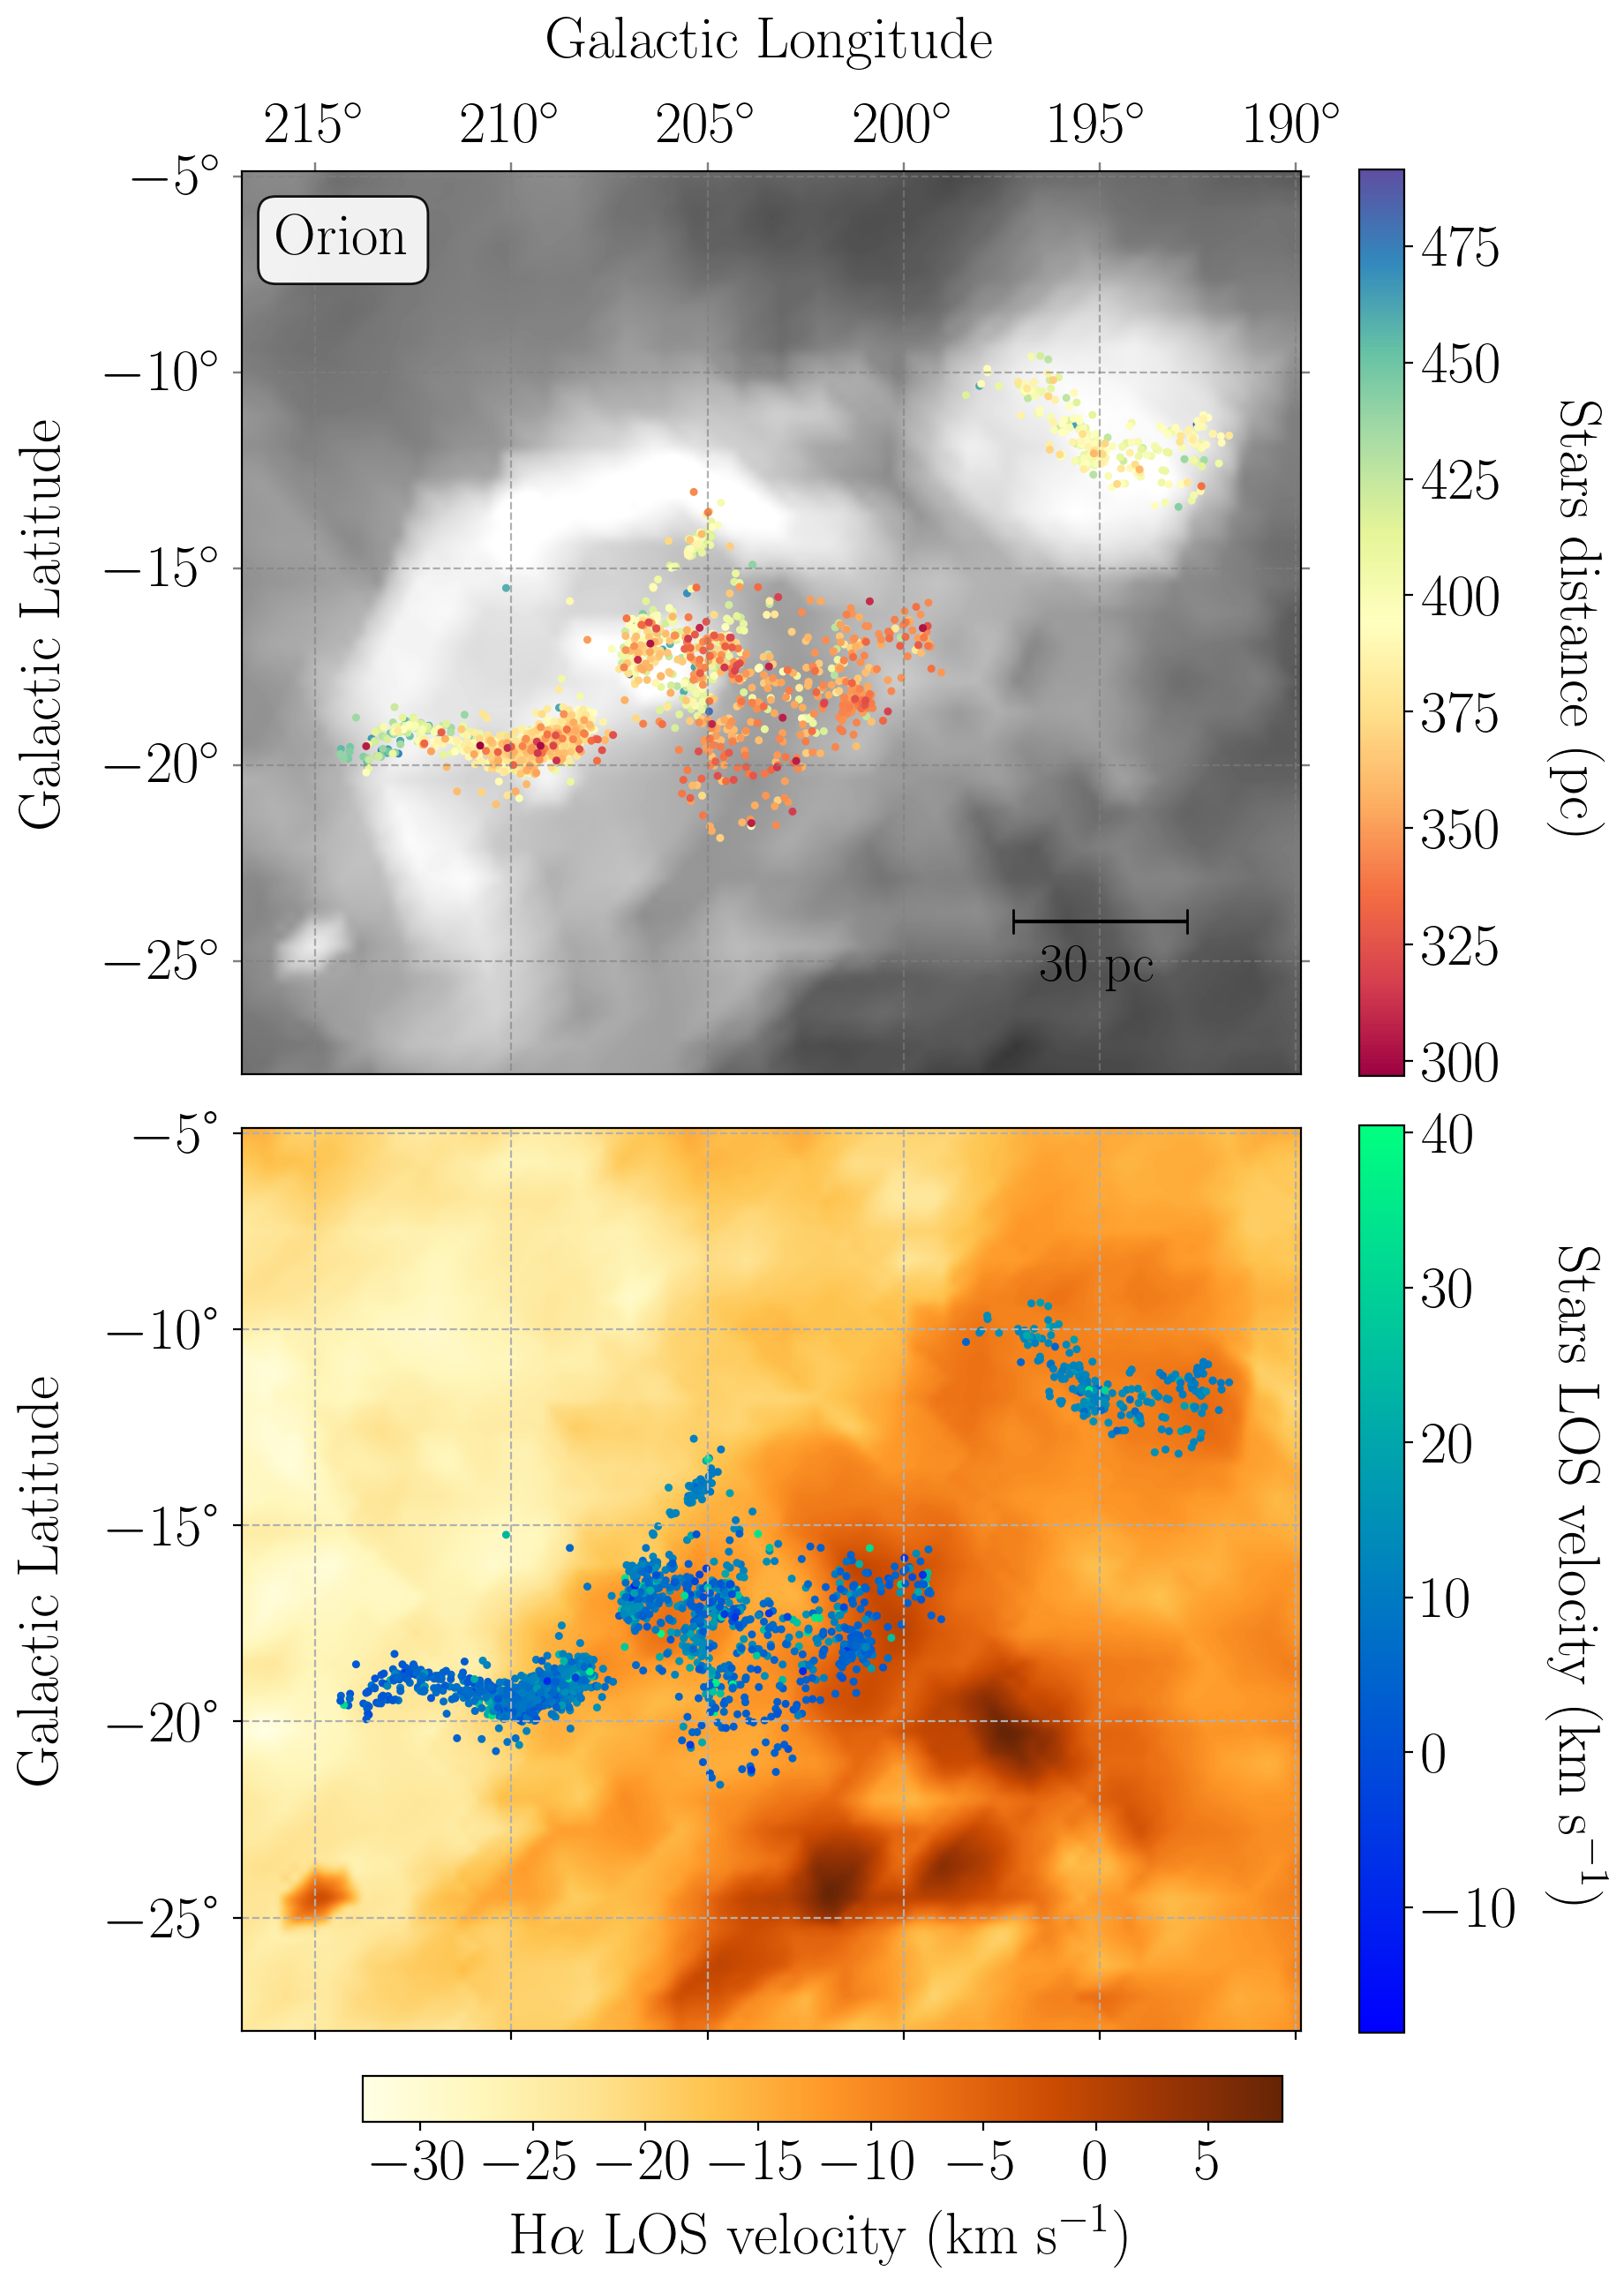
\includegraphics[width=0.37\linewidth,trim=0cm 0cm 0cm 0.2cm, clip=true]{Stars_img/Ori_fig1.png}
    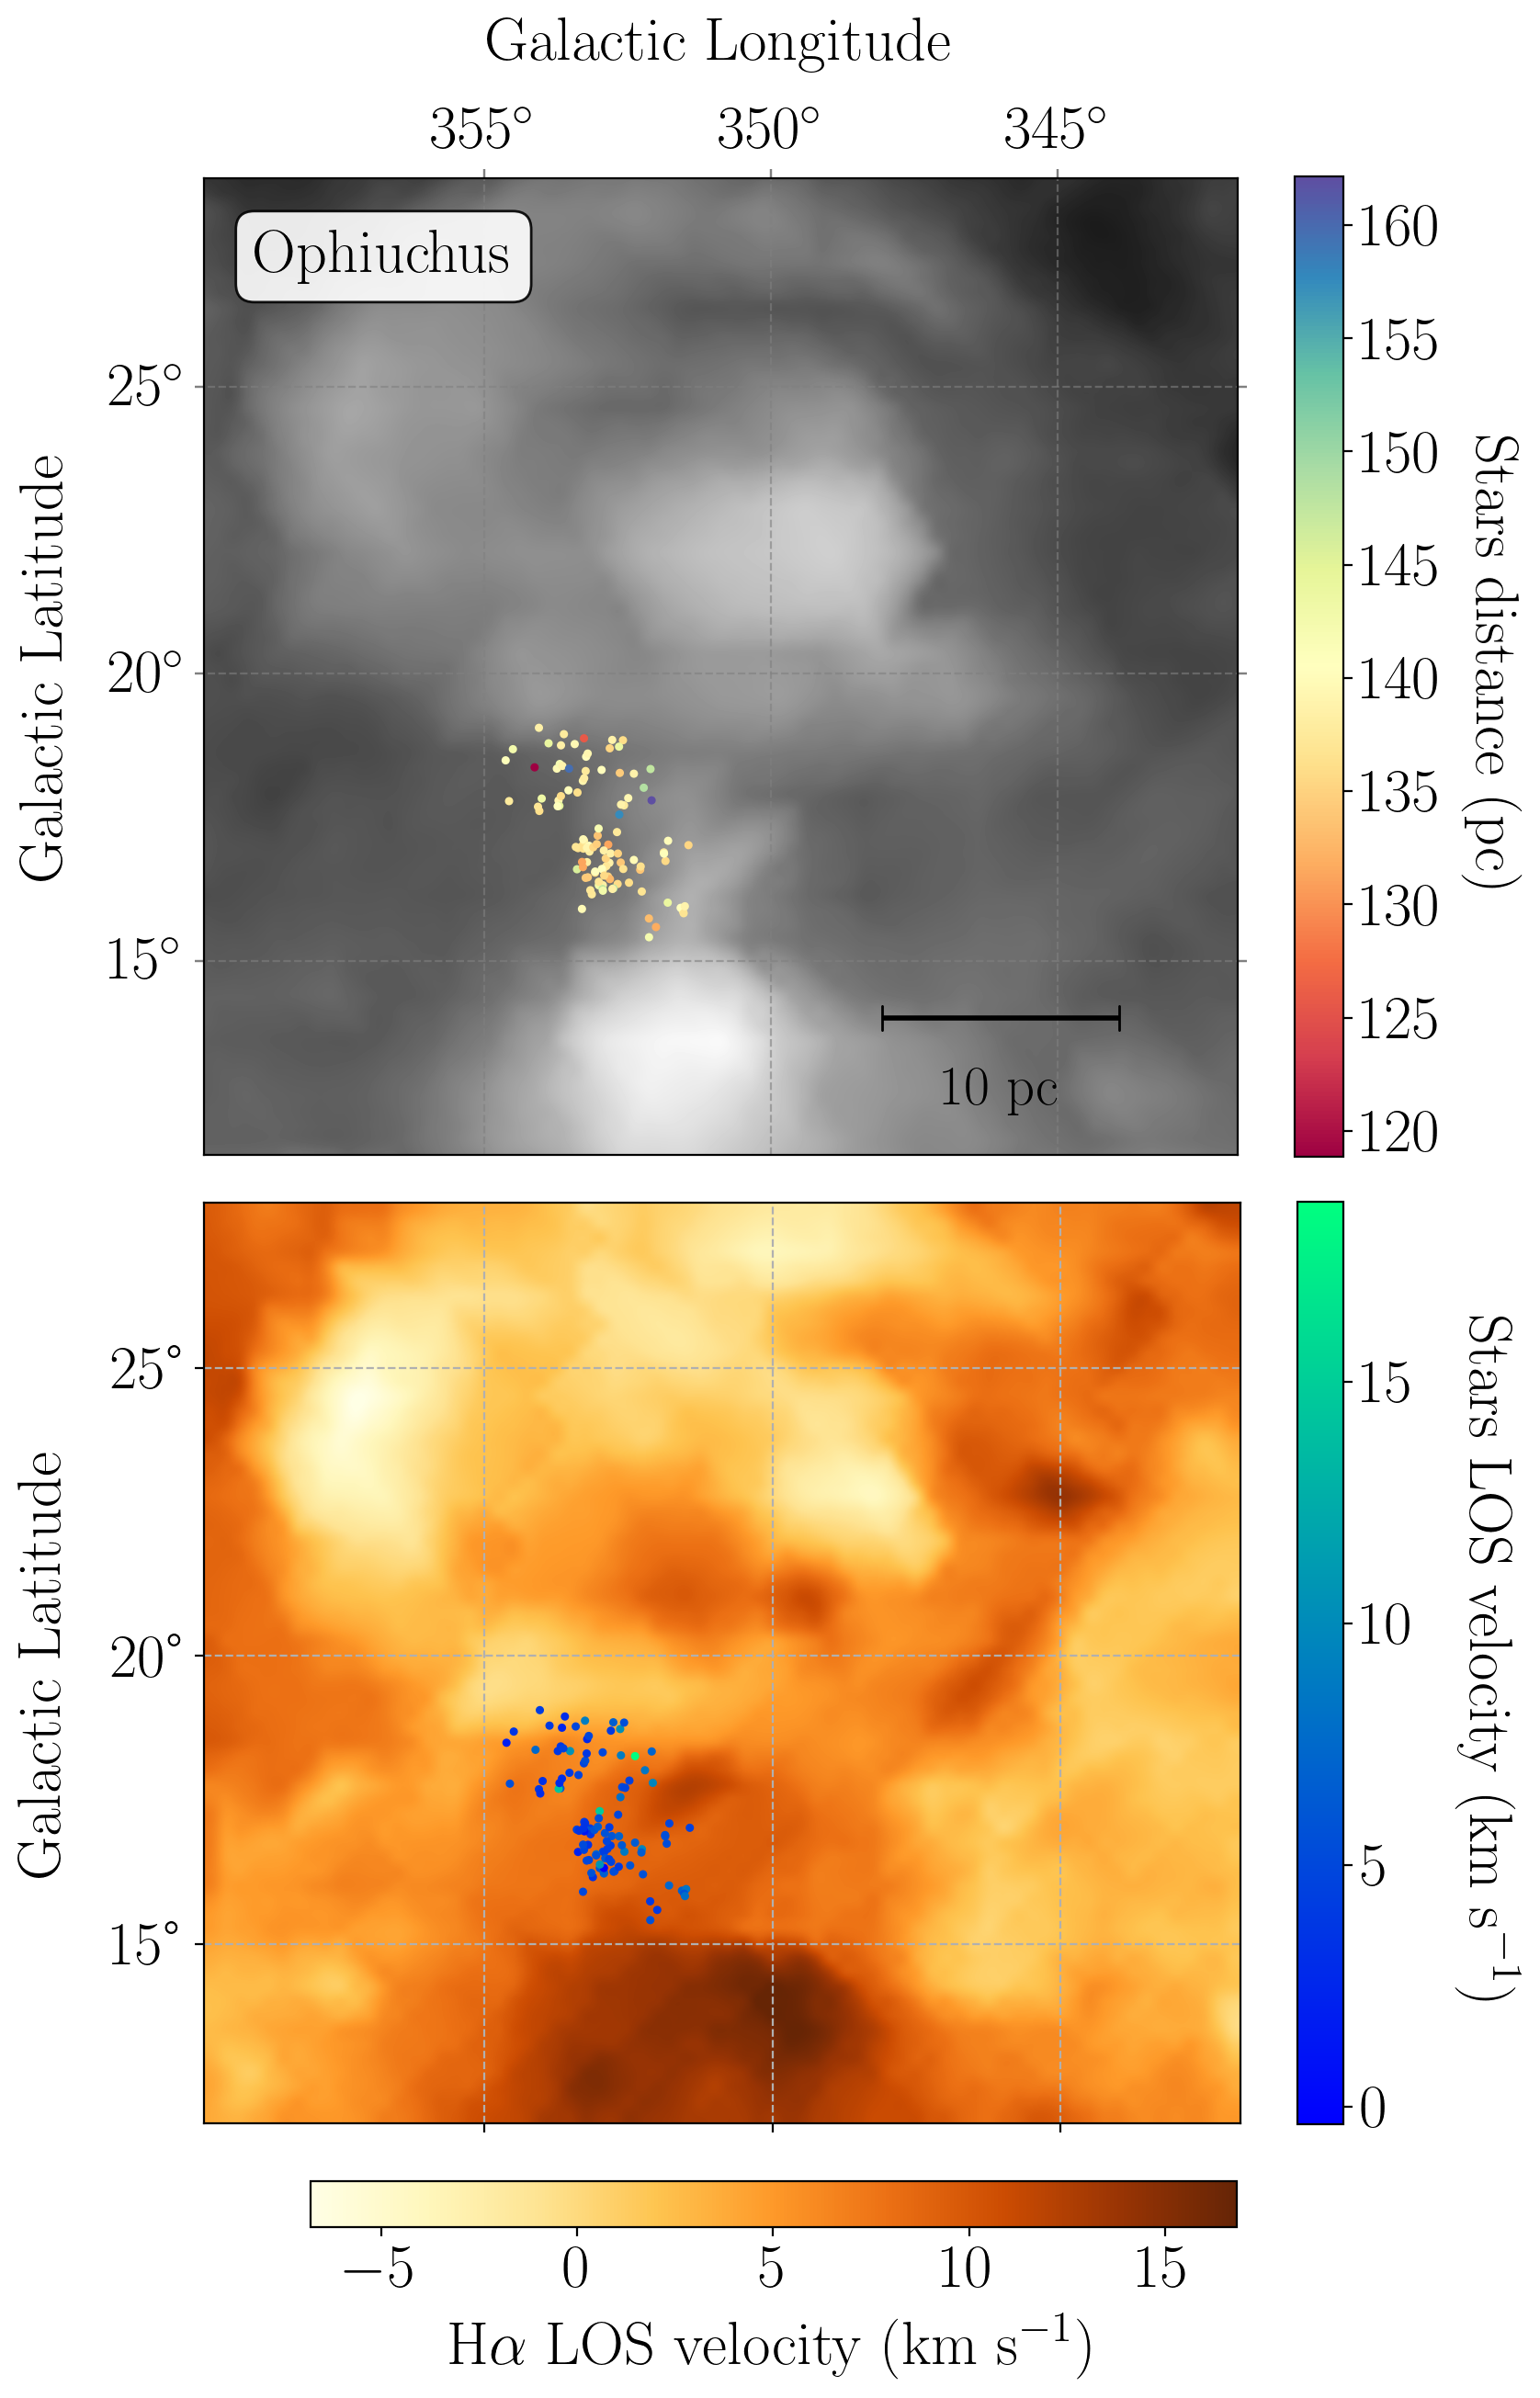
\includegraphics[width=0.312\linewidth,trim=1.5cm 0cm 0cm 0.1cm, clip=true]{Stars_img/Ophi_fig1.png}
    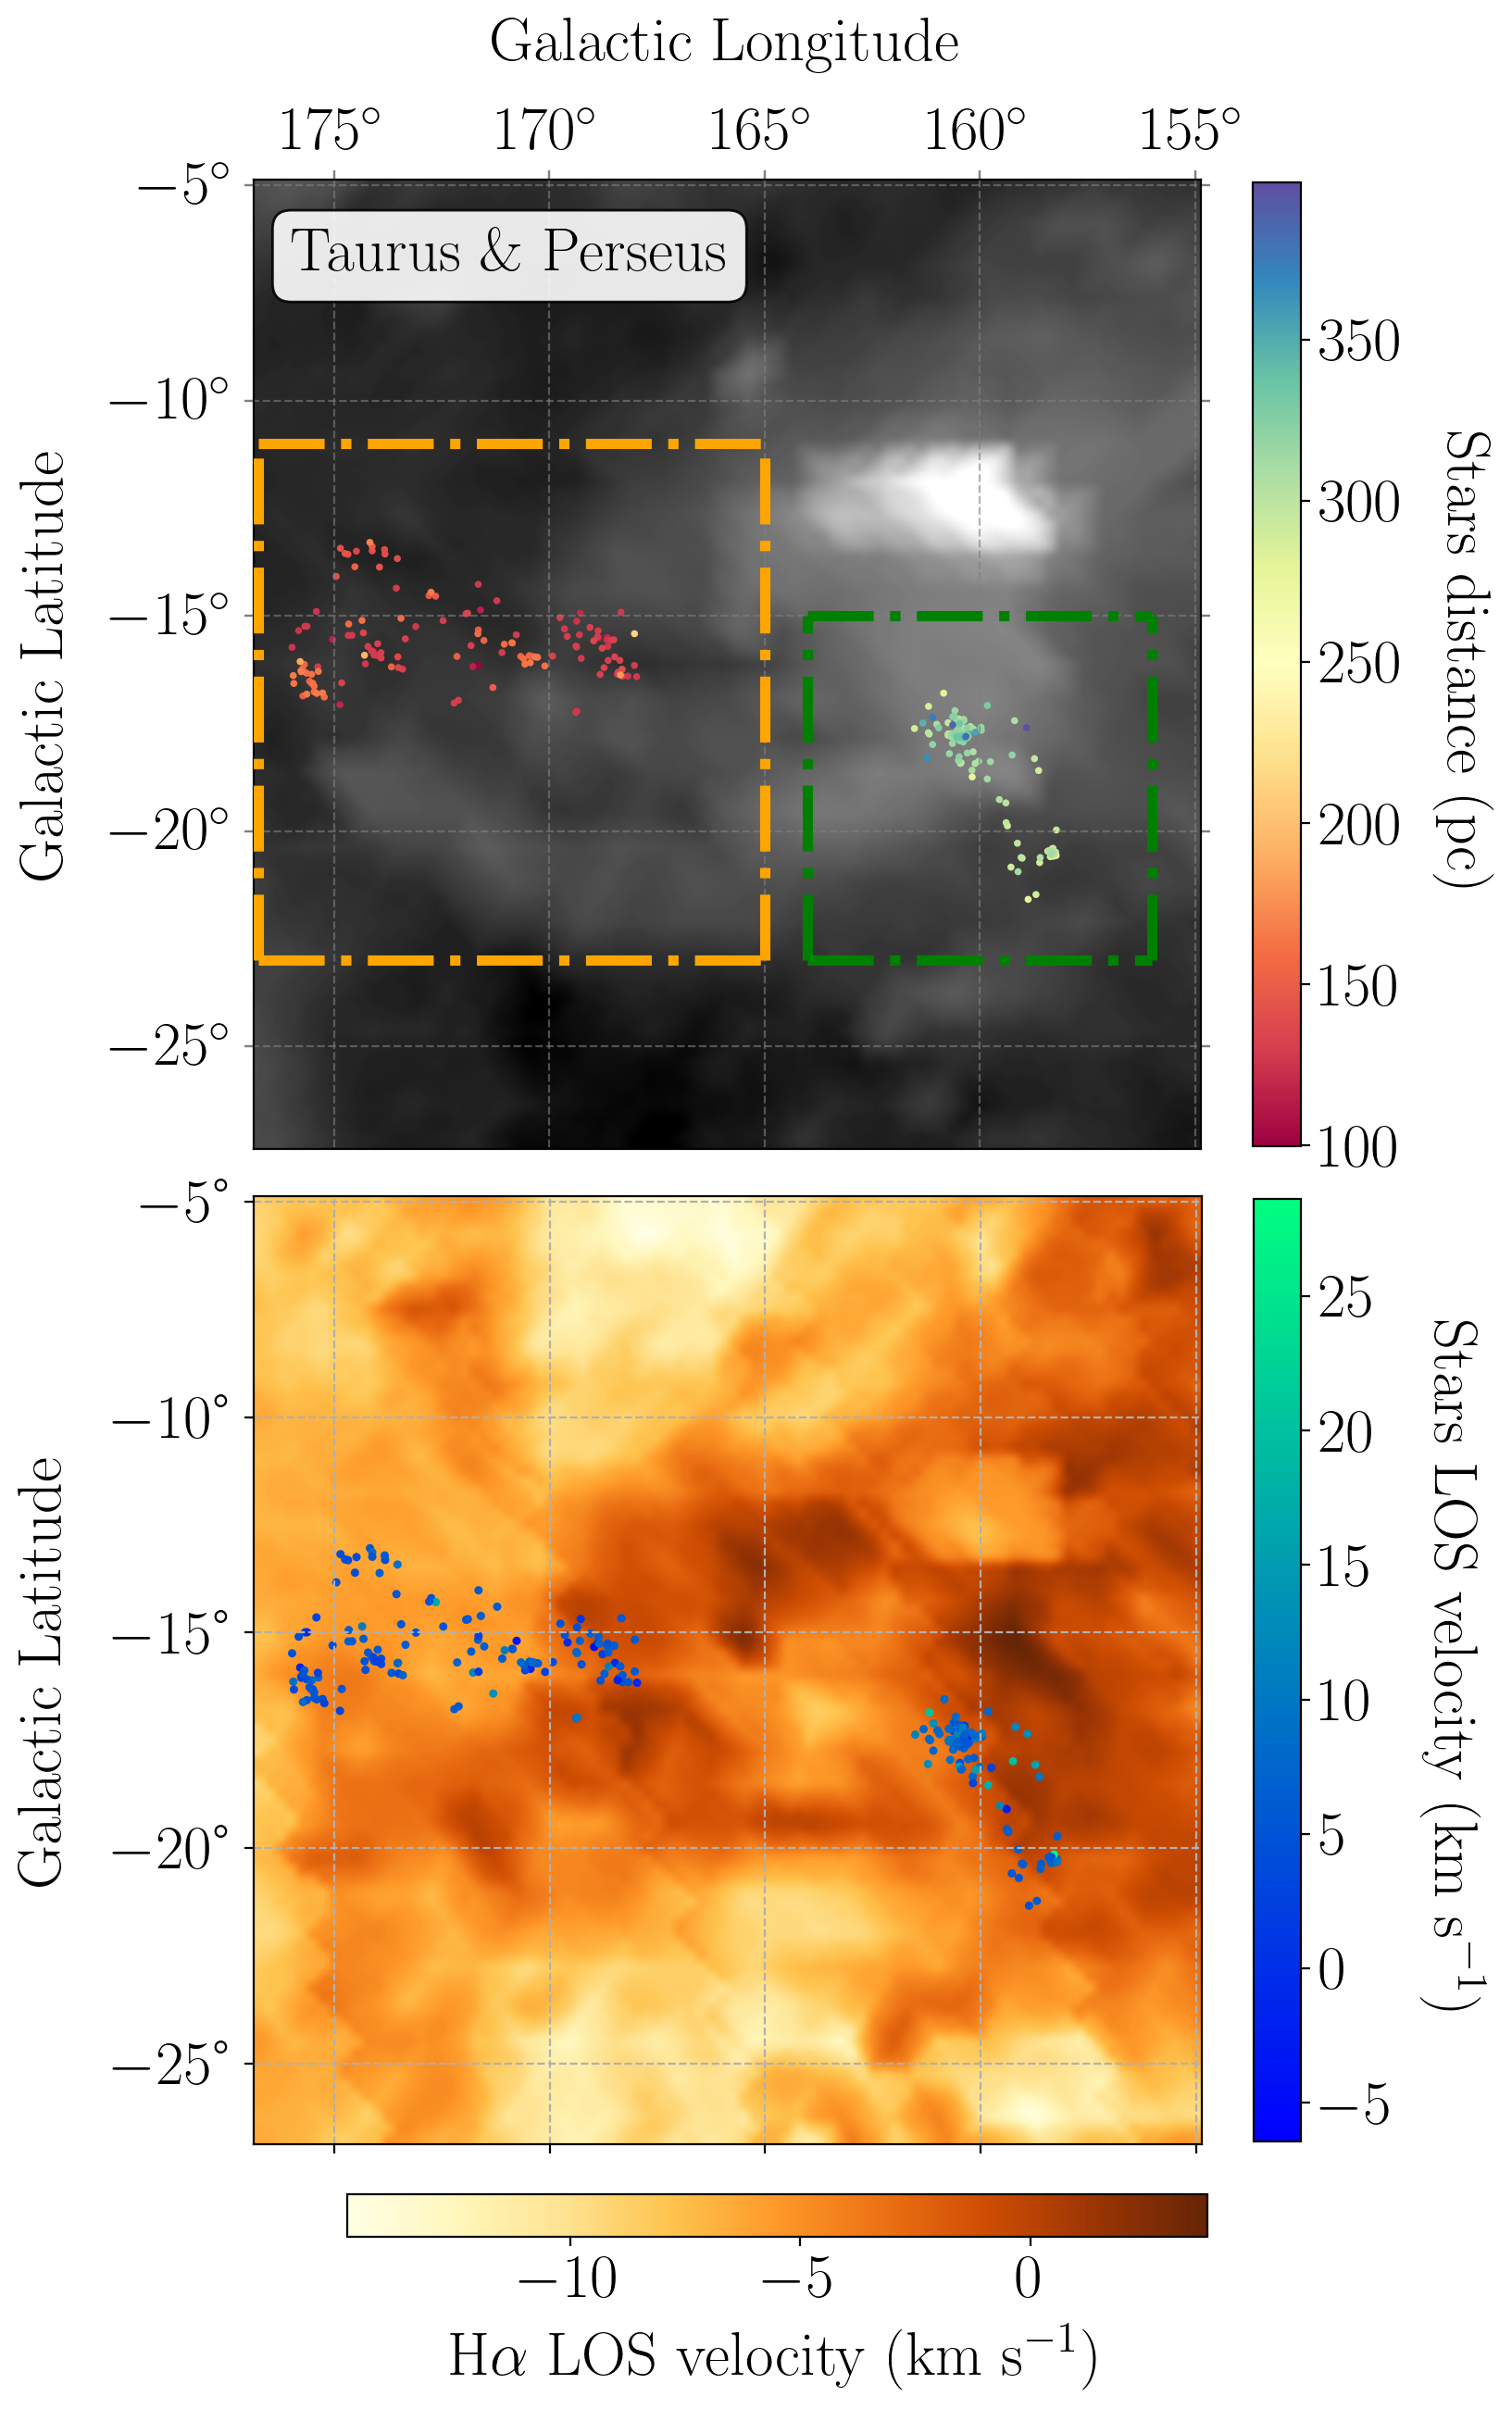
\includegraphics[width=0.302\linewidth,trim=1.6cm 0cm 0.1cm 0.1cm, clip=true]{Stars_img/PerTau_fig1.png}
    \caption{Top panels: positions of young stars color-coded by their distances in Orion, Ophiuchus, Taurus-Perseus (from left to right). Background shows \halpha~flux from the WHAM survey (lighter is brighter). 
    The orange and green boxes denote the areas where \halpha~is analyzed for Taurus and Perseus, respectively.
    Bottom panels show the line-of-sight velocities of the young stars (in the LSR frame) in these regions. The background shows the \halpha~line-of-sight centroid velocities.}
    \label{fig:allsky}
\end{figure*}


\begin{sidewaystable}
    \centering
    \caption{Properties of Star-Forming Regions}
    \label{tab:properties}
    \begin{tabular}{ccccccccc}
        \toprule
        Region        &
        Number of     &
        Number of     &
        Average       &
        GLON          &
        GLAT          &
        Distance      &
        $v_{\rm LSR}$ range          &
        $v_{\rm LSR,~err}$ cut       \\
                      &
        stars         &
        stars used    &
        distance (pc) &
        (\textdegree) &
        (\textdegree) &
        range (pc)    &
        ($\mathrm{km~s^{-1}}$)       &
        ($\mathrm{km~s^{-1}}$)       \\
        \midrule
        Orion     & 2647 & 2468 & 410 & $190,217$ & $-28,-5$  & $300,500$ & $-10,40$ & $10$ \\
        Ophiuchus & 113  & 107  & 140 & $342,360$ & $12,28$   & $120,170$ & $-30,30$ & $2$  \\
        Perseus   & 159  & 138  & 320 & $156,164$ & $-23,-15$ & $250,400$ & $-6,30$  & $10$ \\
        Taurus    & 157  & 139  & 140 & $165,177$ & $-23,-11$ & $97,200$  & $-5,25$  & $5$  \\
        \bottomrule
    \end{tabular}
    \parbox{\linewidth}{\footnotesize \textit{Note.} Number of stars are all 
    the stars with 6D information. Number of stars used are the stars in our 
    analysis after excluding outliers. GLON (Galactic Longitude) and GLAT 
    (Galactic Latitude) ranges denote the borders of windows used to compute 
    the \halpha~VSF\@. The distance ranges, $v_{\rm LSR}$~ranges, and
    $v_{\rm LSR,~err}$~cuts are applied to the stars to exclude outliers.}
\end{sidewaystable}

\subsection{Observations, Data reduction, and Methods} \label{sec:data_method}
\subsubsection{Observations and Data Analysis} \label{sec:alldata}

\centerline{\textbf{Stellar observations}}

We obtain the locations, parallax distances, and proper motions of stars from the Gaia mission \citep{collaboration_gaia_2016} in four nearby star-forming regions: the Orion Molecular Cloud complex (Orion), the \rophi~dark cloud (Ophiuchus), the Perseus molecular cloud traced by two clusters, NGC 1333 and IC 348 (Perseus), and the Taurus molecular clouds (Taurus). The Gaia catalog includes five-parameter astrometric measurements (plane-of-sky coordinates, proper motions, and parallax distances) of over 1.46 billion stars in the Milky Way. Only a very limited subset ($\sim 7$ million) has line-of-sight velocities measured by Gaia. The five-dimensional astrometric data for our four regions are obtained from Gaia's third early data release \citep[EDR3;][]{brown_gaia_2021}. 

The line-of-sight velocities of the stars in our study were observed in the near infrared with the Apache Point Observatory Galactic Evolution Experiment (APOGEE) spectrograph, mounted on the 2.5 m Sloan Foundation Telescope of the Sloan Digital Sky Survey. APOGEE-2 Data Release 17 (DR17) collected high resolution spectral image of over 657,000 stars in the Milky Way \citep{gunn_25_2006,blanton_sloan_2017,abdurrouf_seventeenth_2022}. Combining these two surveys provides six-dimensional (6D) information (3D positions and 3D velocities) of stars for the four molecular clouds.

The stars in our study were assigned to each of the four region by \citet{kounkel_untangling_2019}. They performed a clustering analysis on Gaia DR2 sources in the Milky Way using Python implementation of HDBSCAN \citep[Hierarchical Density-Based Spatial Clustering of Applications with Noise;][]{mcinnes_hdbscan_2017}. We crossmatch this catalog with Gaia EDR3 and APOGEE-2 to obtain 6D astrometries of the stars. 

Then, we exclude a small number of stars whose parallax distances $d$, line-of-sight velocities $v_{\rm LSR}$, and line-of-sight velocity errors $v_{\rm LSR,~err}$~are more than 4$\sigma$~deviated from the mean of the distribution. In Taurus, one star with very high reported proper motion ($v_{\rm LSR,~RA} > 100\mathrm{~mas~yr}^{-1}$) is excluded.
The ranges of $d$~and $v_{\rm LSR}$, and the threshold of $v_{\rm LSR,~err}$~that we use, as well as the total number of stars before and after the cut are specified in Table \ref{tab:properties}. We note, however, that the exact cut of these ranges do not affect the conclusion of this work.

\centerline{\textbf{\halpha~observations}}

The \halpha~data in our study comes from the WHAM survey \citep[][]{haffner_wisconsin_2003,haffner_early_2010}. We obtained the data cubes from the ``DR1-v161116-170912" release, which comprises more than 49000 spectra divided into an irregular grid with a spatial resolution of 1\textdegree, and the data cube is Nyquist-sampled with $4\times4$~pixels per resolution element \citep[][]{haffner_wisconsin_2003}. The intensity of the \halpha~emission is recorded in a 3-dimensional array encoding its Galactic longitude, Galactic latitude, and line-of-sight velocity ($-170$ km s$^{-1} < v_{\rm LSR} < 160$ km s$^{-1}$). We fit a Gaussian distribution to the flux profile along individual lines of sight. Then we take the velocity at the peak of the distribution as the centroid velocity and the uncertainty of the fit as the uncertainty. We also correct for Galactic rotation following the procedure in \citet{qu_warm_2020}.

Figure \ref{fig:allsky} shows the \halpha~map of the four regions in our analysis, with stars overplotted as foreground dots. The top panels show the integrated line-of-sight fluxes in log scale. In the foreground, each star is color-coded by their distance from Earth. We note that although Perseus and Taurus are very close to each other on the sky, they are physically separated by $\sim 150$~pc along the line of sight. In the bottom panels, we plot the centroid velocity of the \halpha~in the background, and the line-of-sight velocities of stars in the foreground.

\subsubsection{Data analysis} \label{sec:analysis}

We compute the first-order VSF of stars in each region. The VSF is related to the kinetic energy power spectrum of a velocity field, and is expressed as a two-point correlation function between the absolute velocity differences $|\delta v|$ versus the physical separation $\ell$. For a turbulent velocity field, we expect the VSF to have a characteristic power-law scaling with slope 1/3 for incompressible turbulence dominated by solenoidal motions \citep[][]{kolmogorov_local_1941}, or a slope 1/2 for supersonic turbulence dominated by compressive motions. For the Milky Way molecular clouds, \citet{larson_turbulence_1981} found a relationship between cloud size and velocity dispersion to be $\sigma = 1.1~R^{0.38}$.

The 3D VSF of stars is computed as follows. First, the positions, distances, radial velocities, and proper motions of stars are translated into galactocentric Cartesian coordinates and velocities. Then, for each pair of stars, the absolute velocity vector difference $|\delta \vec v|$ and the distance $d$ between them is calculated. For individual clouds, these distances are sorted into logarithmic bins of $\ell$, and $|\delta \vec v|$ values within a bin are averaged out to obtain \vsf. To estimate uncertainties, we first generate 1000 random samples of stellar parameters following a Gaussian distribution around the reported measurements and with a 1$\sigma$ scatter equal to the reported uncertainties. Then at each $\ell$, we take the 1$\sigma$ value of the 1000 \vsf~to be the uncertainty.

For the WHAM \halpha~data, we first define a rectangular box containing the stars in each of the four regions as specified in Table \ref{tab:properties} and shown in Figure~\ref{fig:allsky}. Our results are not sensitive to the exact size of the box (see Section \ref{sec:windowsize} for detailed discussions). We compute the first-order VSF of each region using the projected position-position-velocity information. The resultant VSF is $\langle |\delta v| \rangle_{\rm proj}$~versus angular separations $\theta$. Then, we assume a constant distance equal to the mean distance of stars in each region (see Table~\ref{tab:properties}) and translate $\theta$~(\textdegree) to $\ell_{\rm proj}$~(pc). Since three degrees of freedom are missing in this projected VSF calculation (the proper motions of gas and its exact distance), we scale $\langle |\delta v| \rangle_{\rm proj}$~and $\ell_{\rm proj}$ by a constant factor, assuming an isotropic turbulent velocity field. 

\begin{equation}
    \langle|\delta \vec v|\rangle = \sqrt{3}~ \langle|\delta v|\rangle_{\rm proj},
\end{equation}
\begin{equation}
    \ell = \sqrt{\frac{3}{2}}~\ell_{\rm proj}.
\end{equation}

\subsection{Results} \label{sec:multi-region-results}

\begin{figure}
	\centering
	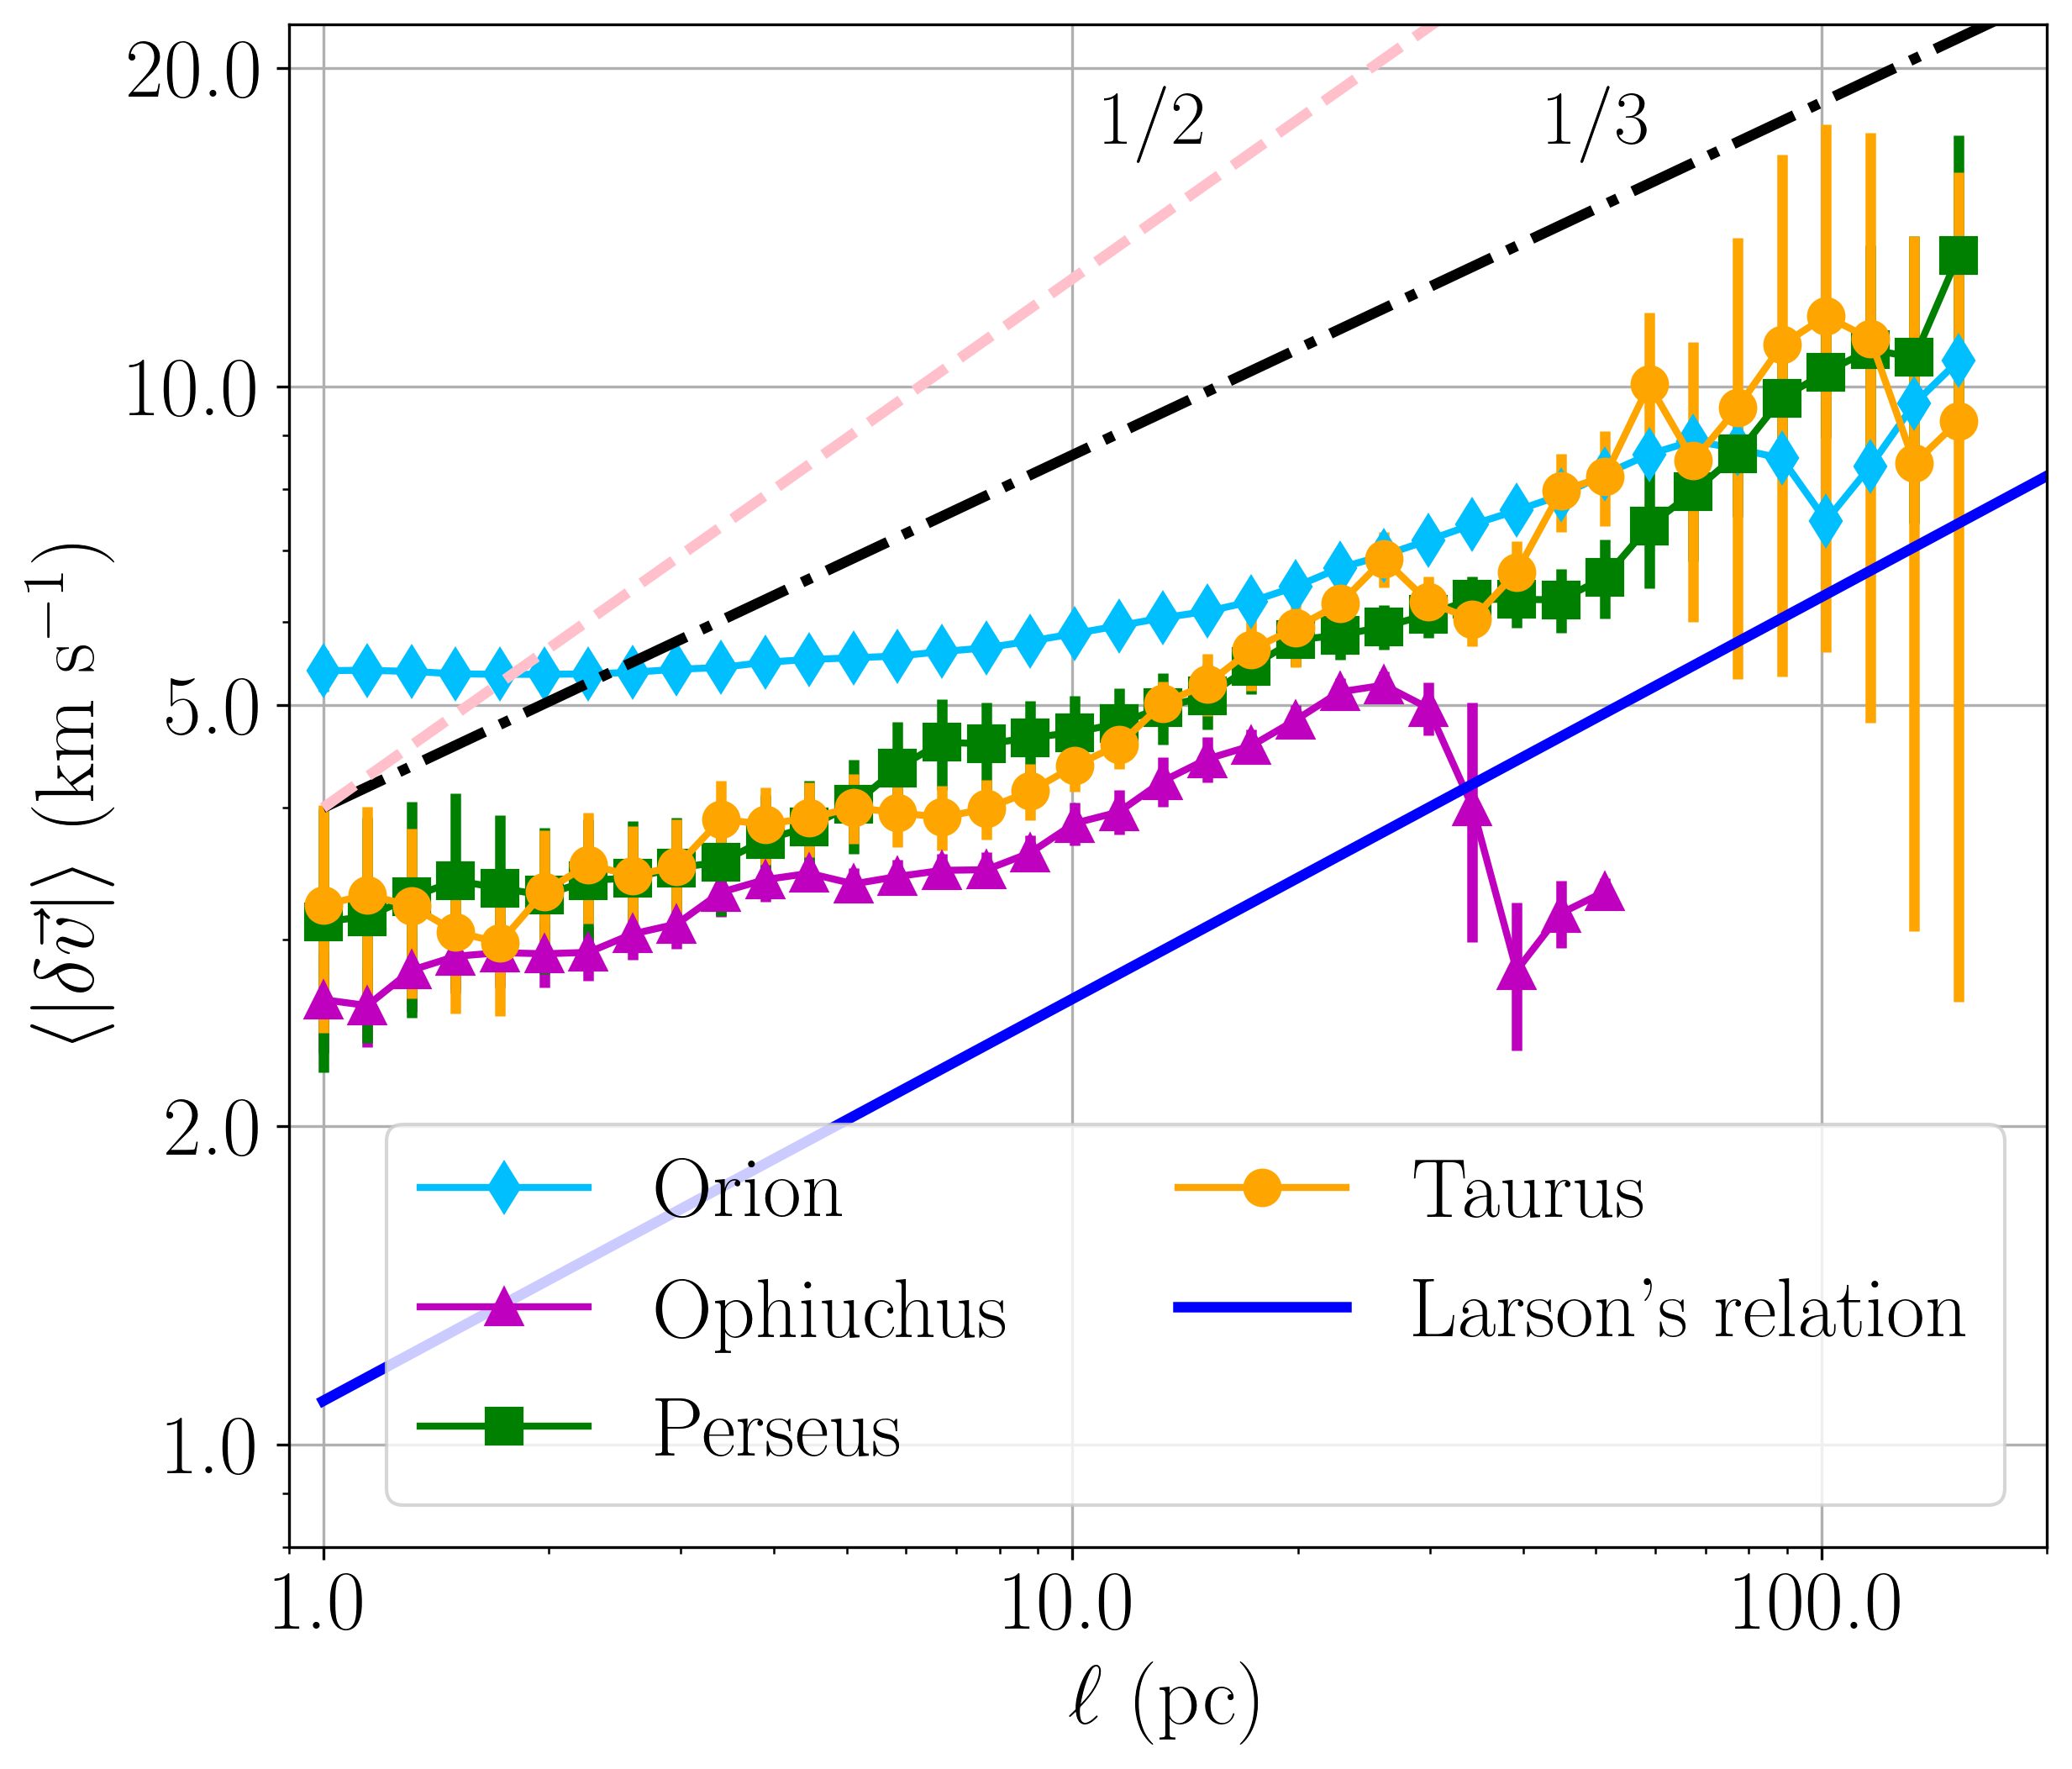
\includegraphics[width=\linewidth]{Stars_img/allstar_vsf_dr17.png}
	\caption{The first-order VSFs of the stars in Orion (light blue), Ophiuchus (magenta), Perseus (green), and Taurus (orange). For reference, we plot a solid blue line for Larson's relation, a black dotted-dashed line for Kolmogorov turbulence, and a pink dashed line for supersonic turbulence. The vertical lines represent the uncertainties in \vsf~ at each $\ell$.}
	\label{fig:starsvsf}
\end{figure}

\subsubsection{The Universality of ISM Turbulence Traced by Young Stars}\label{sec:starvsf}
We first examine the velocity statistics of the four star-forming regions: Orion, Ophiuchus, Perseus, and Taurus. Figure~\ref{fig:starsvsf} shows the VSFs traced by stars of these four regions. For reference, we also plot the Larson's relation of velocity dispersion vs. cloud size, the 1/3 slope of Kolmogorov turbulence, and the 1/2 slope of supersonic turbulence. Immediately, we recognize a remarkable universality among the VSFs of different regions. Over a large dynamical range, the magnitude and slopes of the VSFs show a general agreement with Larson's relation (see Table~\ref{tab:slopes} for the best-fit slopes of the VSFs). This suggests that the motion of young stars in the Milky Way show characteristics of turbulence, and supports our previous findings in Paper I that turbulence in the ISM can be traced with young stars.

At $\ell \lesssim 10$~pc, the slopes of the VSF of all four regions are flatter than Larson's relation, as well as Kolmogorov (slope 1/3) turbulence. We discuss the possible cause of this flattening in Section~\ref{sec:star_discussion}.

\subsubsection{The VSFs of Individual Regions} \label{subset:eachregion_result}

\begin{figure*}[ht!]
    \centering
    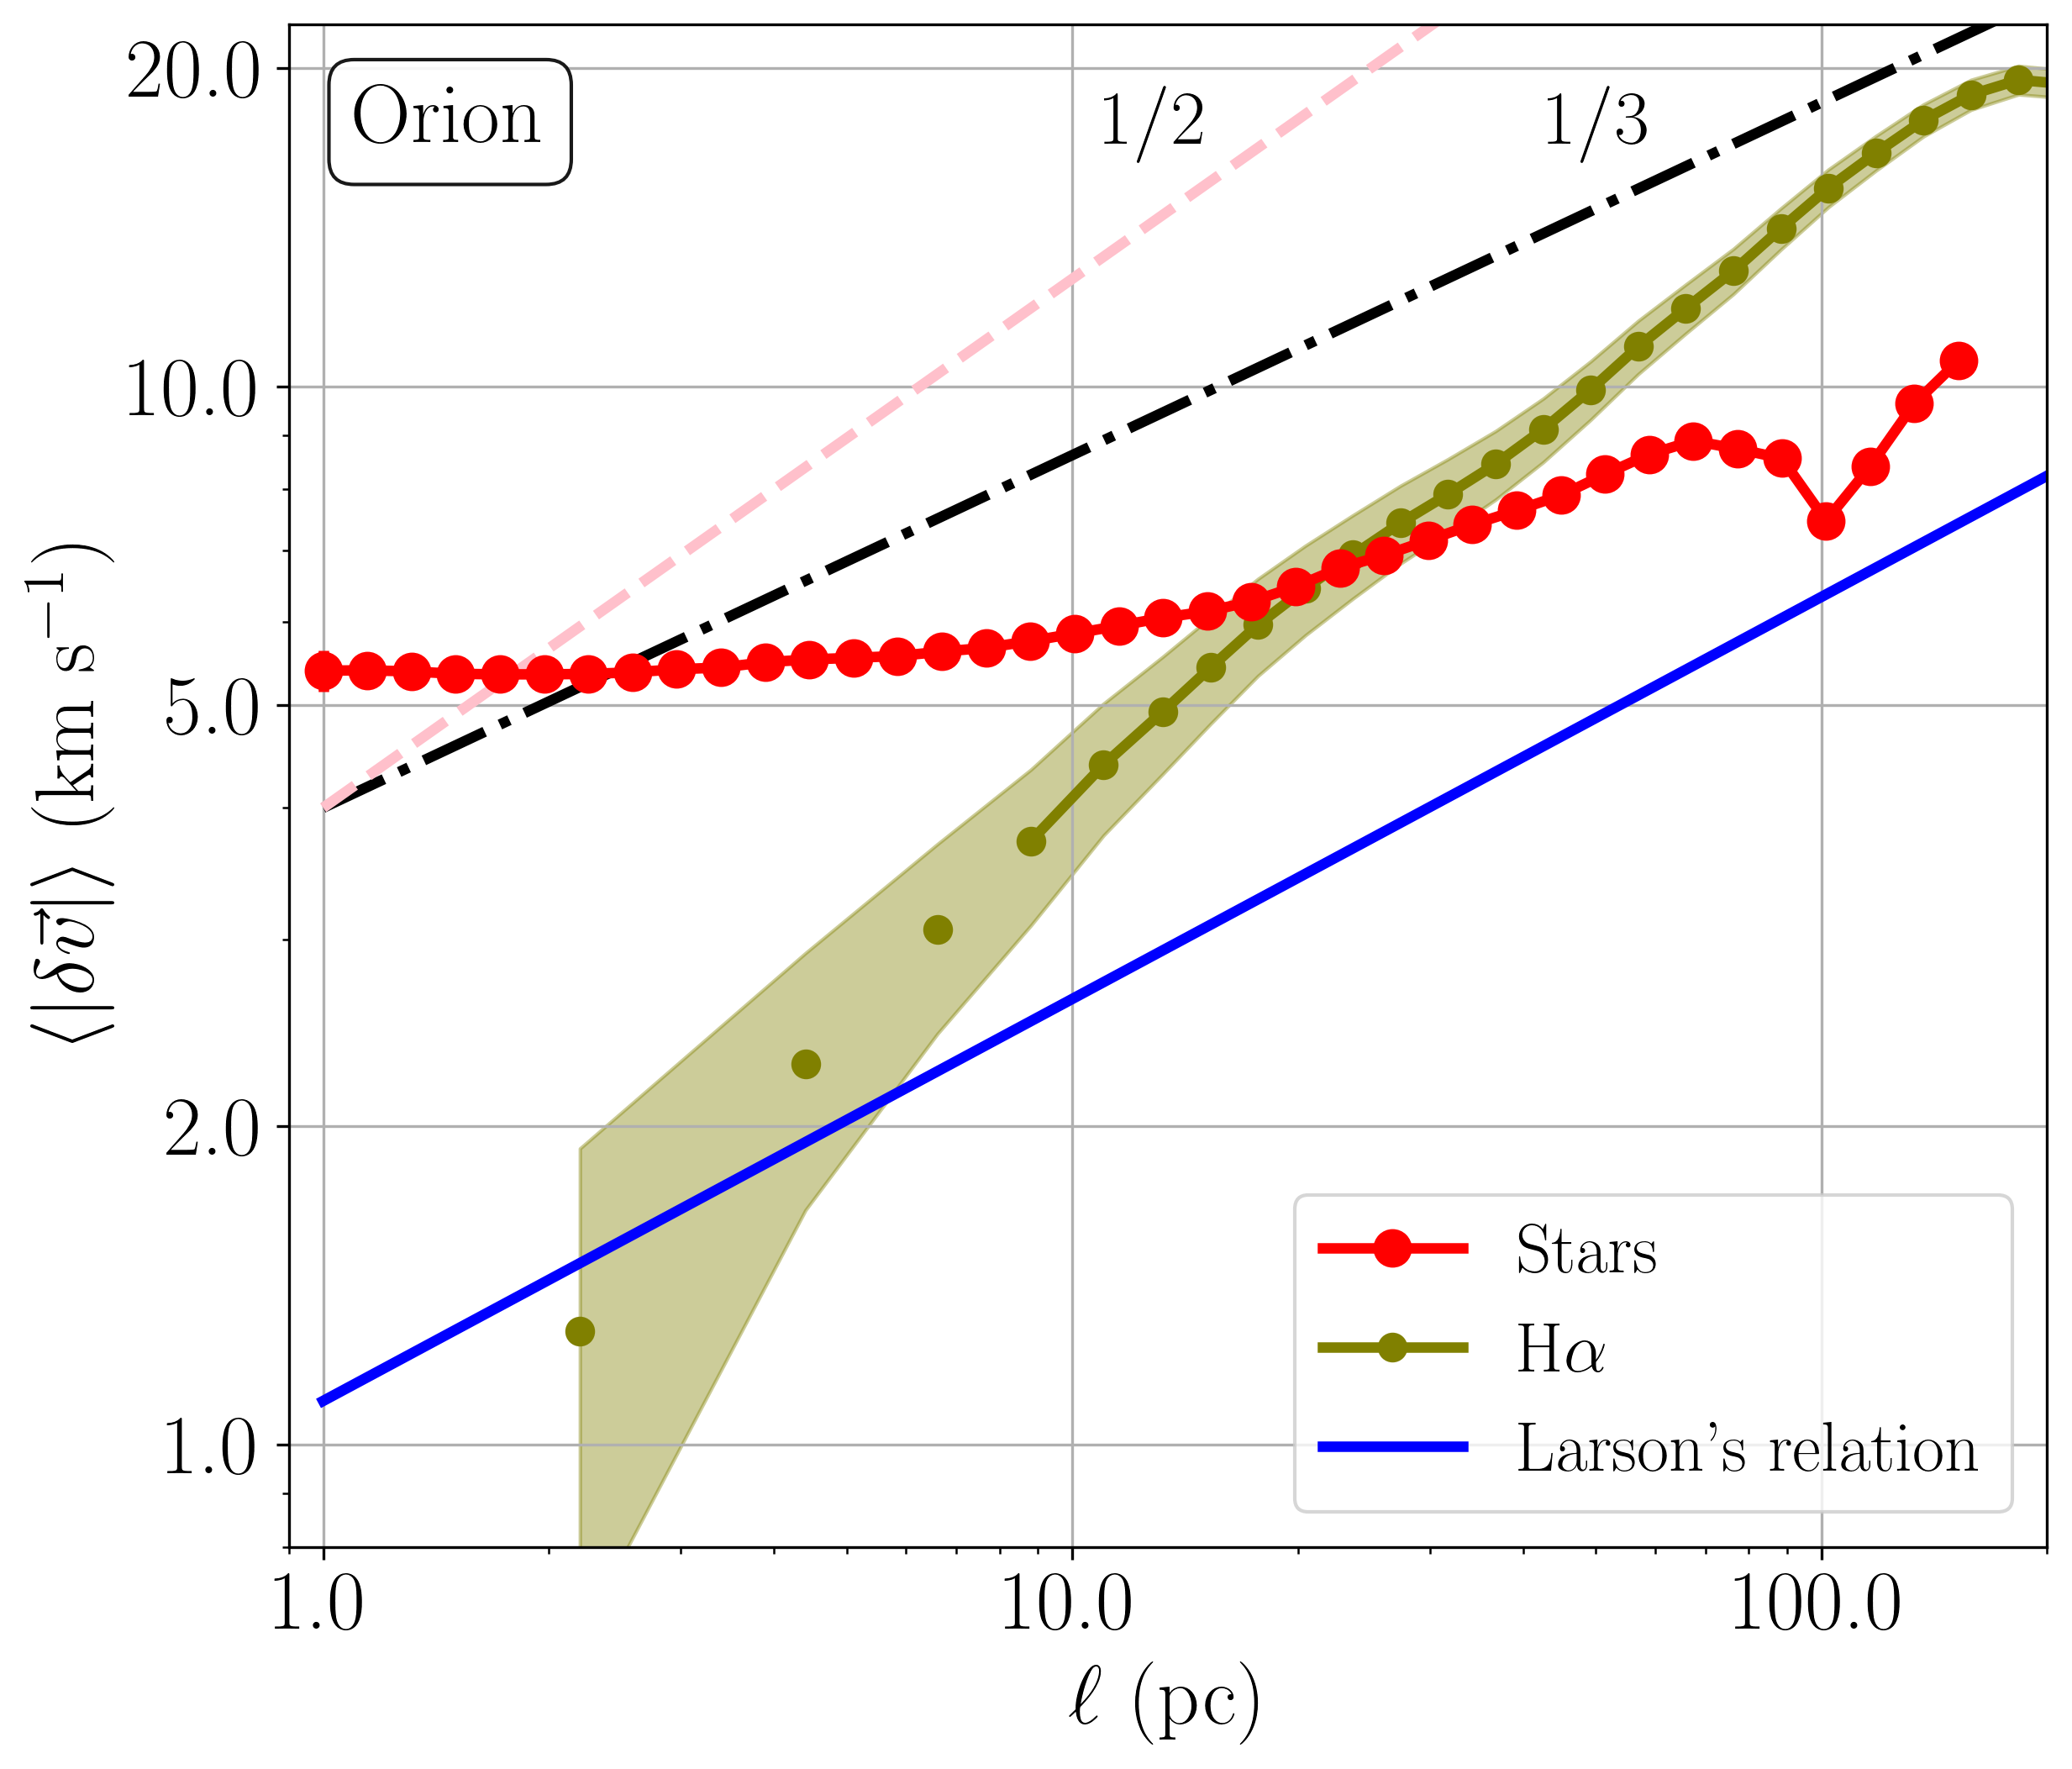
\includegraphics[width=0.48\linewidth]{Stars_img/Ori_fill.png}
    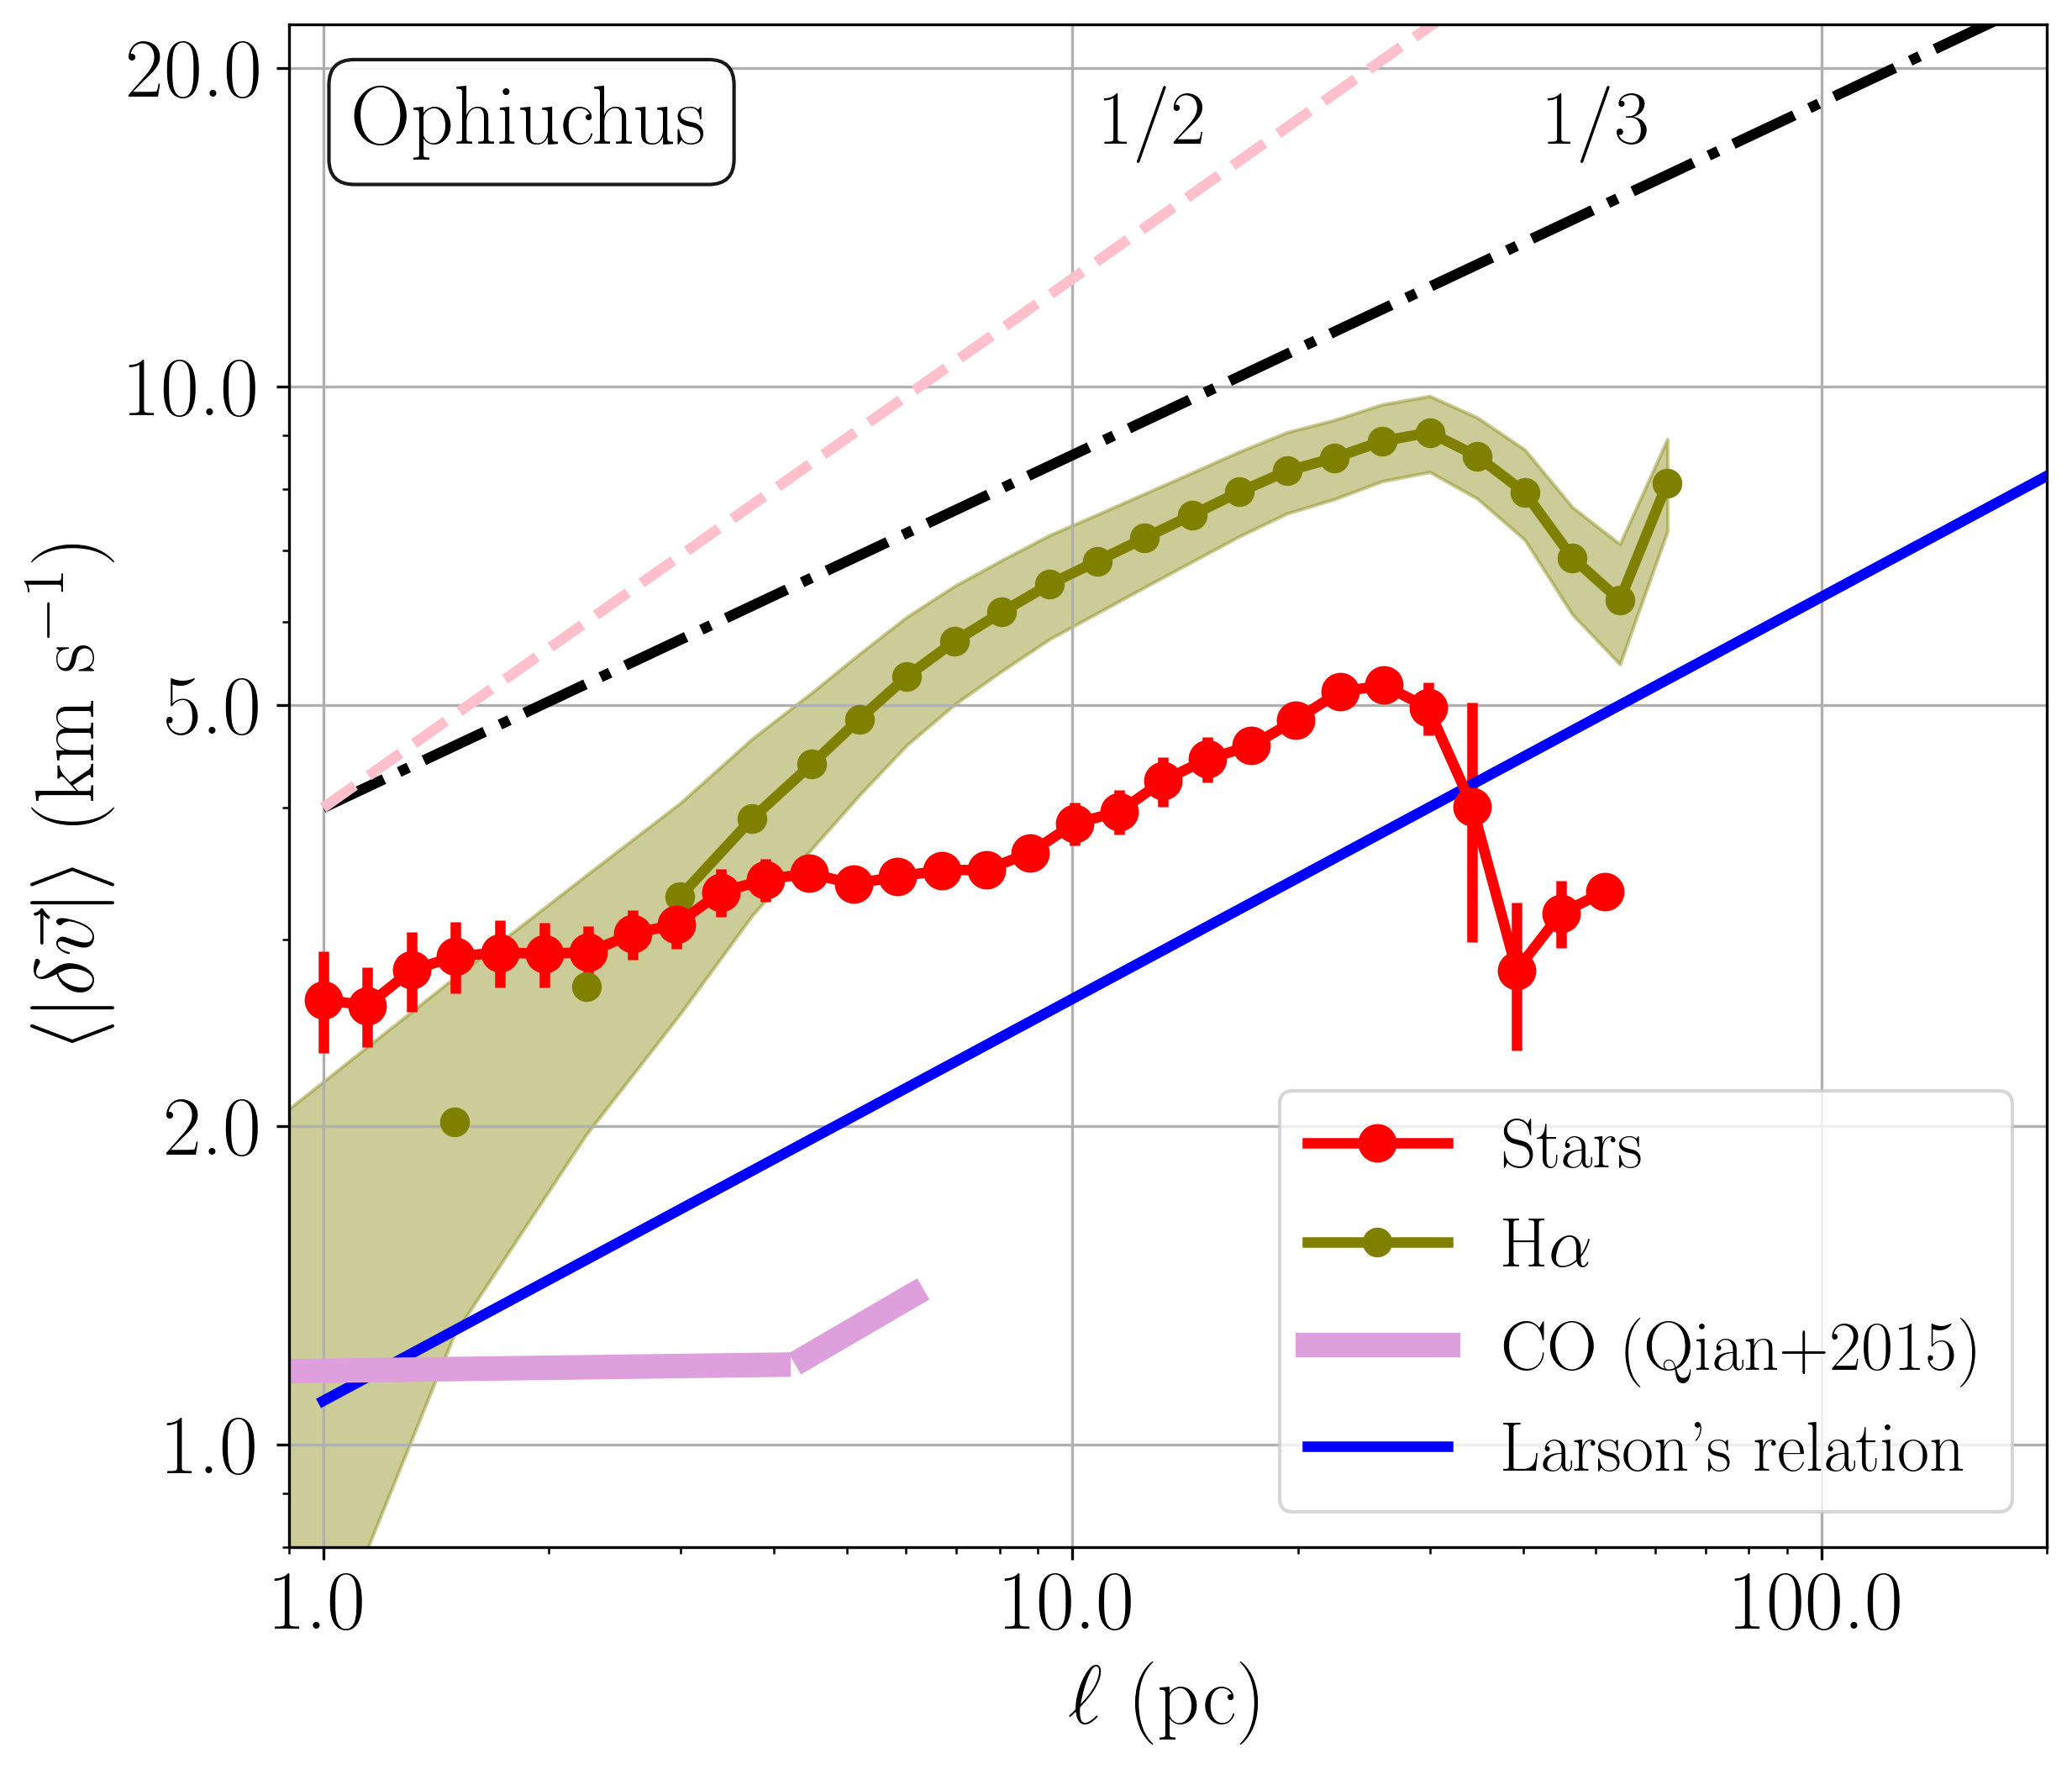
\includegraphics[width=0.48\linewidth]{Stars_img/Ophi_fill.png}
    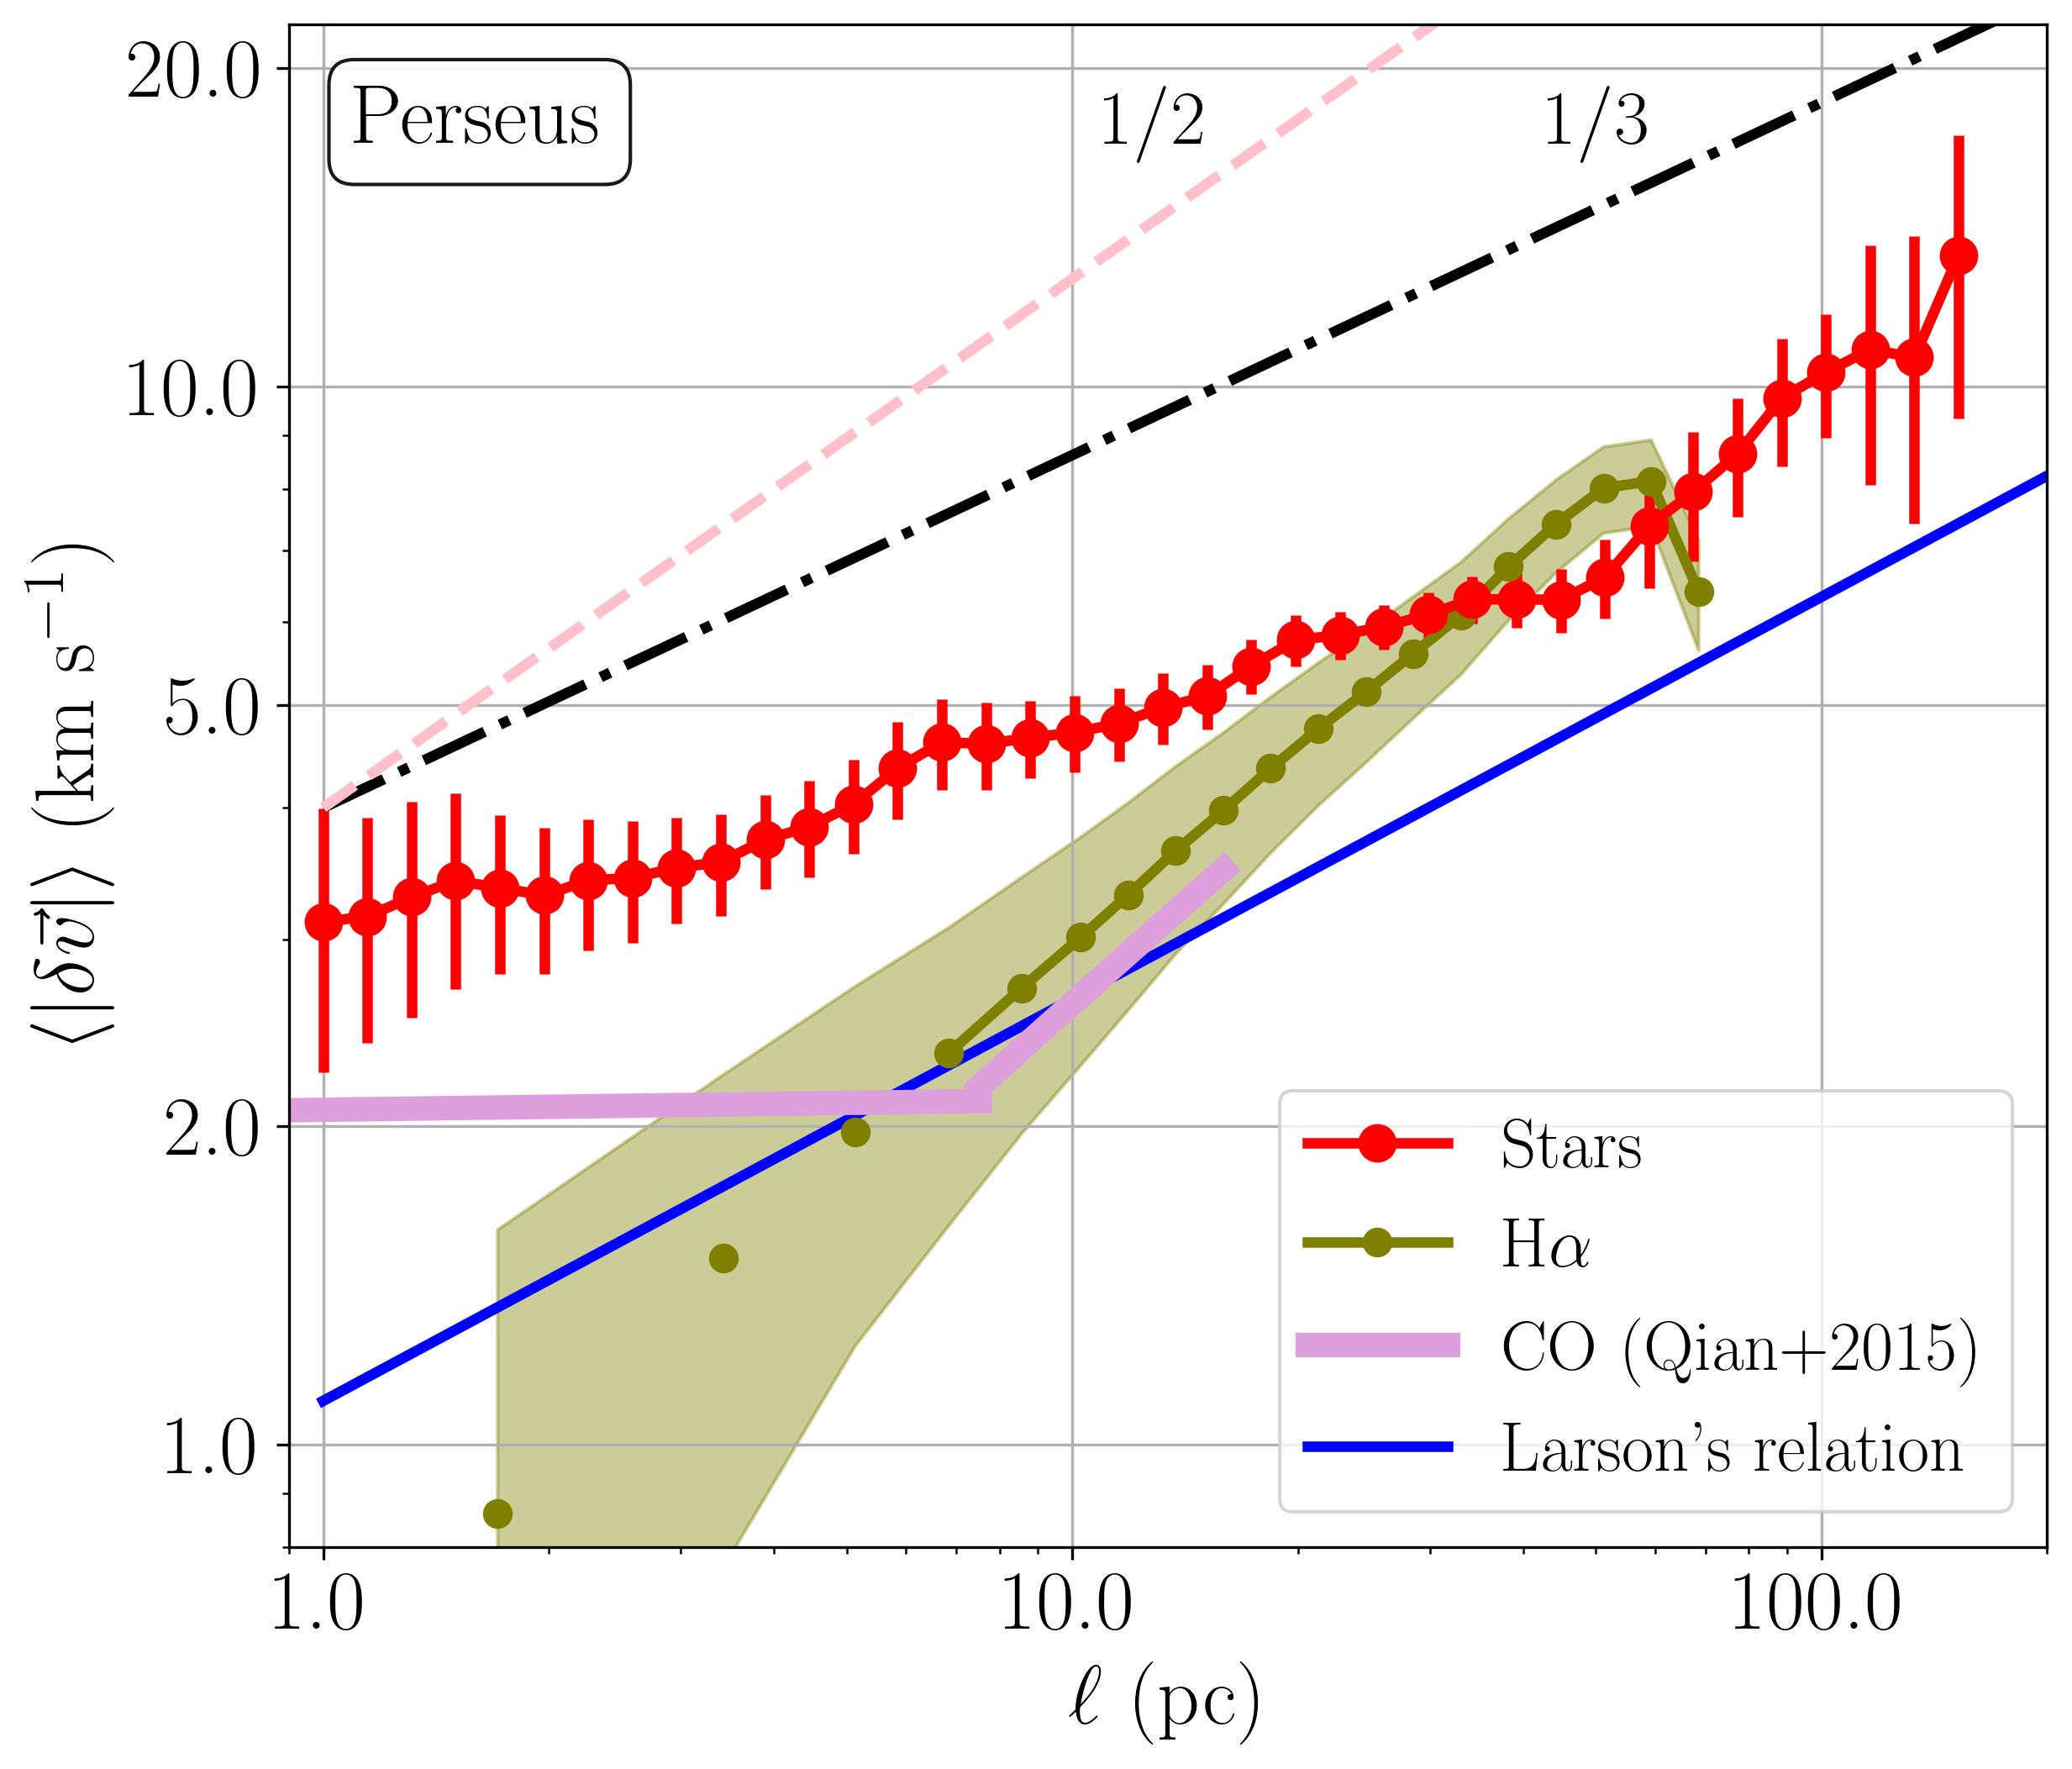
\includegraphics[width=0.48\linewidth]{Stars_img/Per_fill.png}
    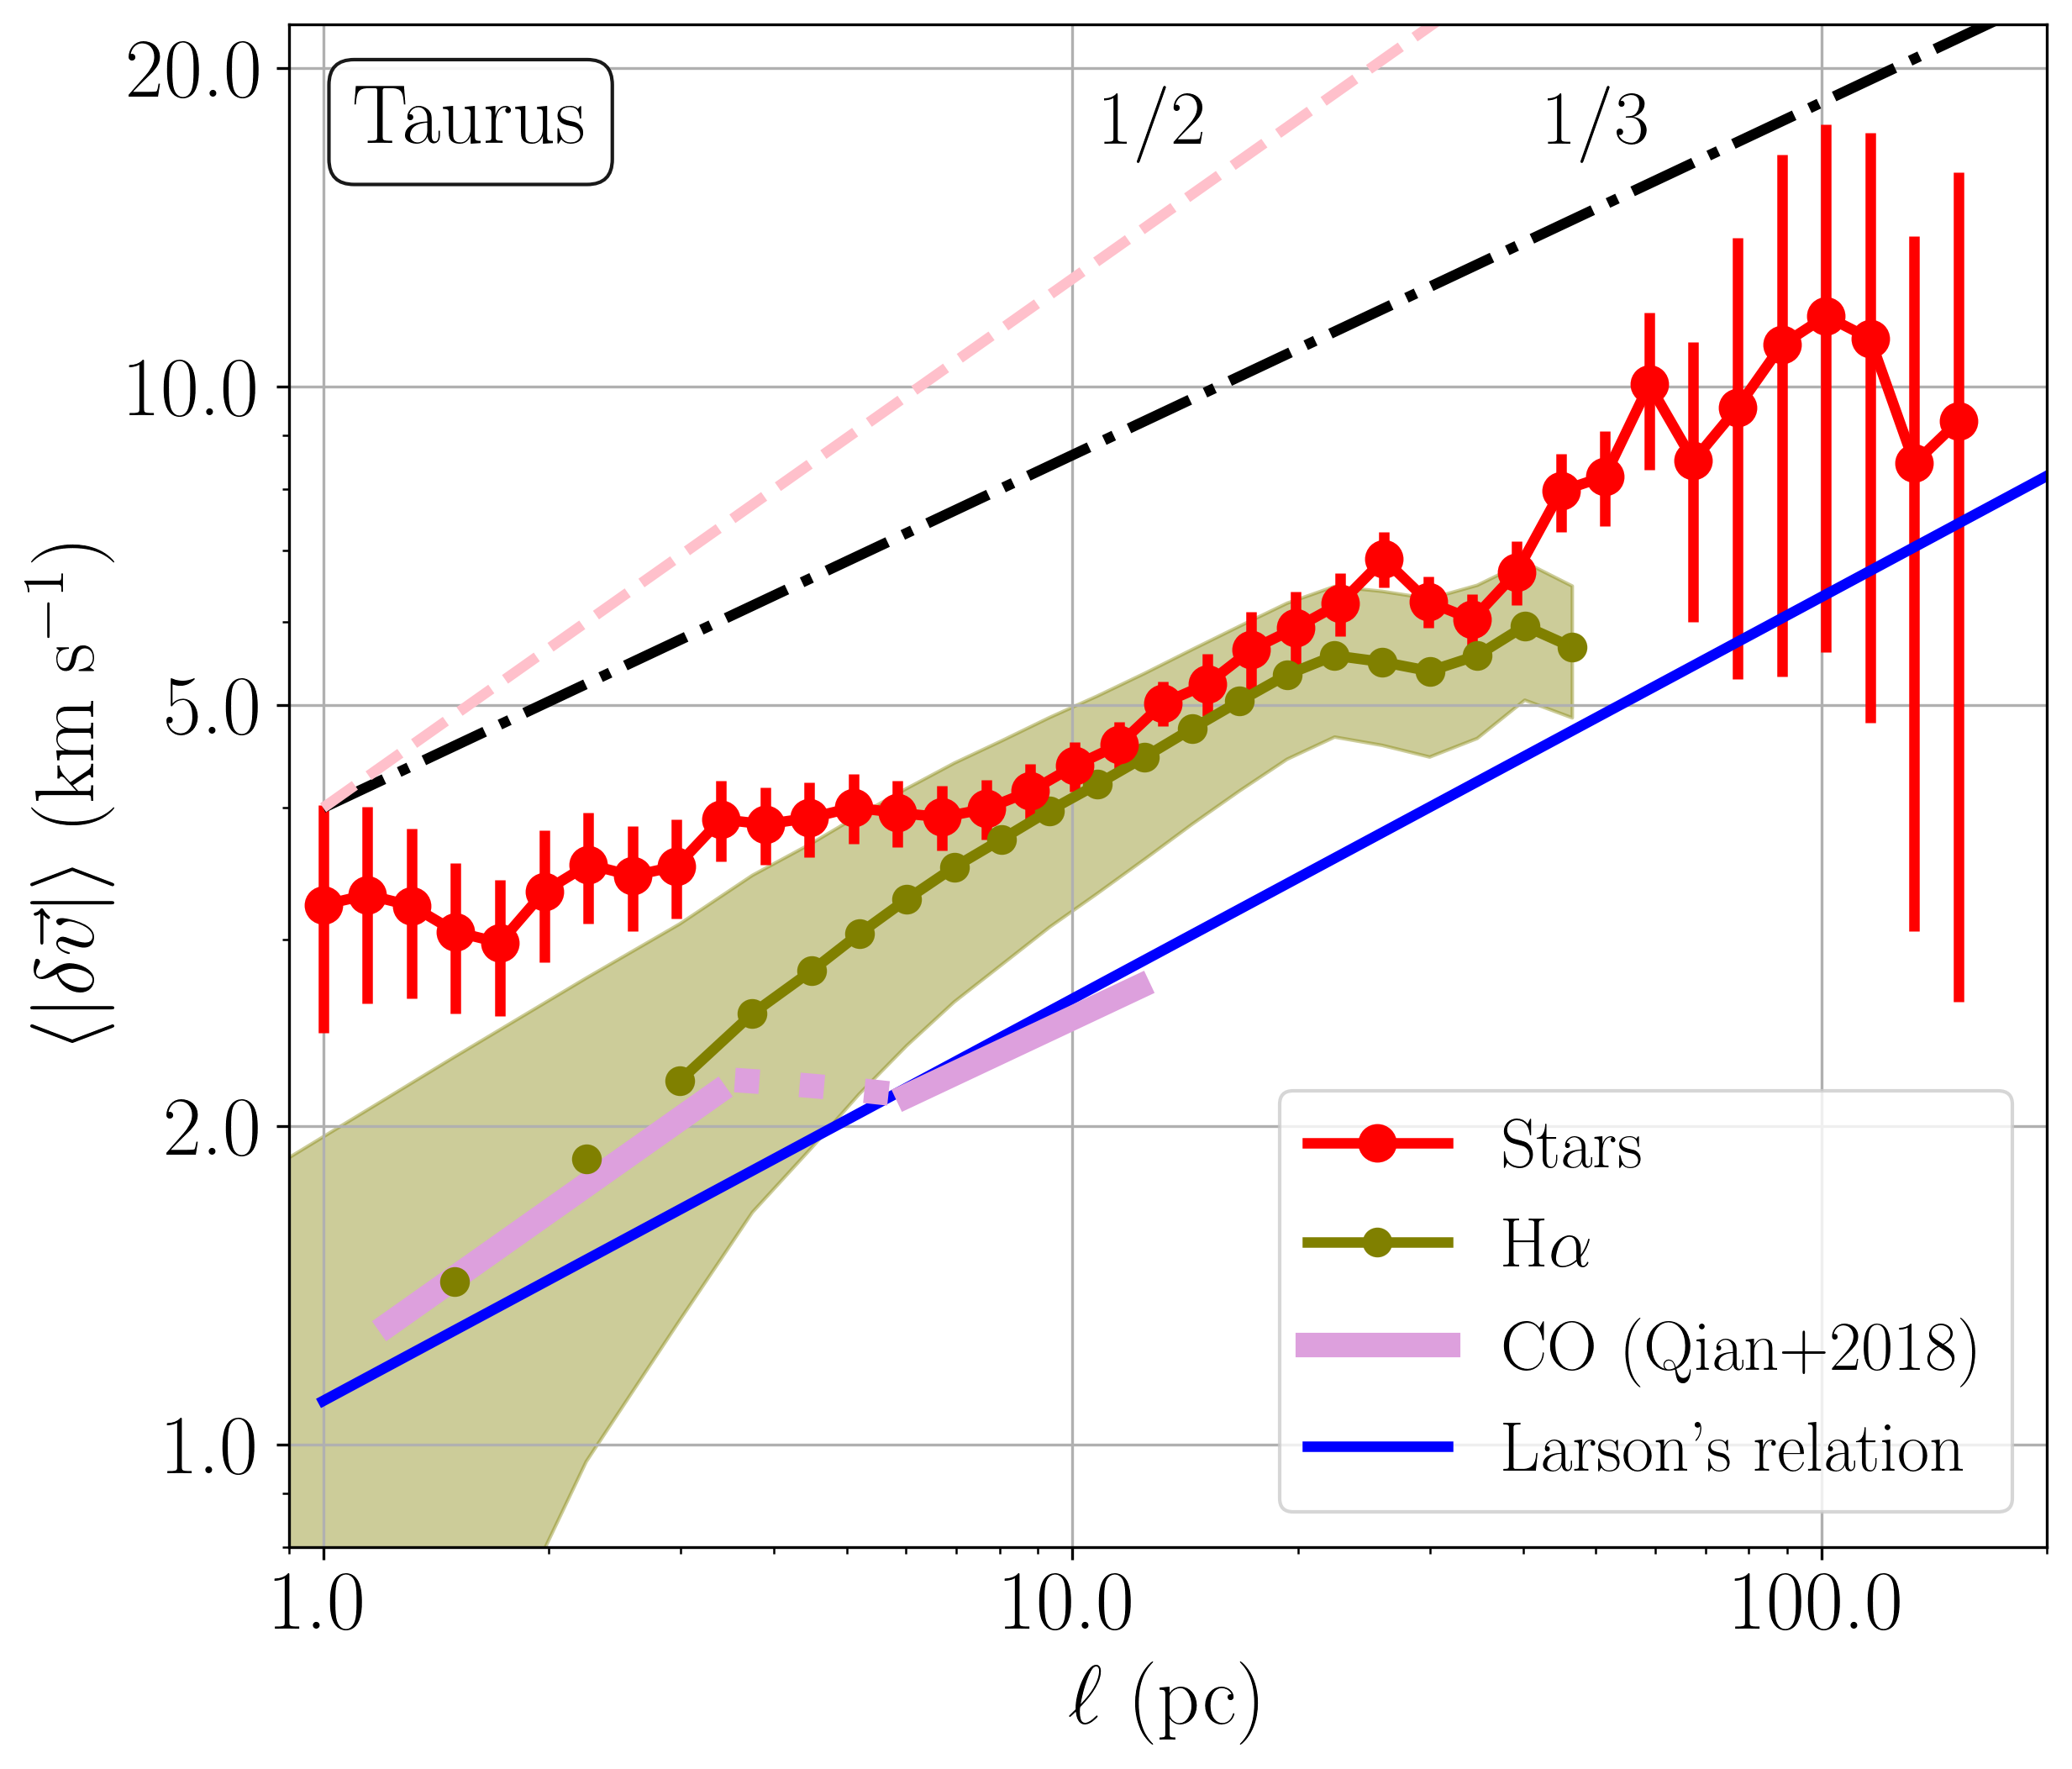
\includegraphics[width=0.48\linewidth]{Stars_img/Tau_fill.png}
    \caption{The first-order 3D VSF of stars (red) and H$\alpha$ (olive) for Orion, Ophiuchus, Perseus, and Taurus. The shaded region around the \halpha~VSF is its associated uncertainty. At small $\ell$, the dots showing the VSF traced by \halpha~are not connected to indicate the resolution limit of the WHAM survey ($\theta < 1$\textdegree). The slopes of the VSFs of stars and of \halpha~are specified in Table \ref{tab:slopes}. The VSF of \halpha~in Ophiuchus~can also be fitted with a broken power-law, with slope $0.58 \pm 0.24$ for $3~\mathrm{pc} < l < 9$~pc and slope $0.29 \pm 0.08$ for $9~\mathrm{pc} < l < 30$~pc. For comparison, we also include CO (violet) analysis from \citet{qian_new_2015,qian_studies_2018} for three of these regions.}
    \label{fig:stars_gas}
\end{figure*}

Figure \ref{fig:stars_gas} shows the VSFs of young stars as well as gas in each of the four regions: Orion, Ophiuchus, Perseus, and Taurus. The best-fit slopes of these VSFs are lists in Table~\ref{tab:slopes}.

\centerline{\textbf{Orion}}

The first-order VSF of Orion traced by stars has been studied in detail in Paper I. We only reiterate some of the main points here and address the differences caused by the addition of $\sim 1000$~stars compared with Paper I. 
Throughout the inertial range, the magnitude of $\langle |\delta \vec{v}| \rangle$~is higher than Larson's relation. At small scales ($1~\mathrm{pc} \lesssim \ell \lesssim 20$~pc), the number statistics is dominated by stars in the Orion Nebula Cluster (ONC), which flattens the VSF (see Section~\ref{sec:star_discussion} for more discussion on the small-scale flattening). 
At ranges from $20$~pc to $\sim 70$~pc, Orion D, which is a loose stellar association at the front of the Orion Complex along our line of sight, dominates the statistics, and it exhibits a power-law scaling, which indicates an imprint of turbulence from their natal molecular clouds. The VSF of Orion without considering the ONC would be steeper at small scales, which renders it more in-line with the VSF of other regions (see Figure \ref{fig:starsvsf}).
At $\sim 70$~pc, there is a bump in the structure function, and we proposed that this is an evidence supporting the existence of a SN explosion at the heart of Orion 6 Myr ago \citep{kounkel_supernovae_2020}.
Paper I used Gaia DR2 only. The newly added stars in this study from Gaia EDR3 have larger overall uncertainty in their parametric solutions. Therefore, the noise floor for Orion at small scales is boosted from $\sim 3$~km s$^{-1}$ to $\sim 5$~km s$^{-1}$. This slightly elevates the overall VSF compared to the values in Paper I.

\halpha~emission in Orion mainly comes from the Barnard's loop and the $\lambda$~Ori bubble (see Figure~\ref{fig:allsky}), which are thought to be created by SN explosions \citep{kounkel_supernovae_2020}. We see the effect of such energy injection in the VSF traced by \halpha. At $\ell \gtrsim 20$~pc, the amplitude of the \halpha~VSF is higher than the VSF of young stars. Over the whole dynamical range we probe here, the \halpha~VSF has a roughly constant slope of 1/2. 

The VSF traced by \halpha~shows a bump at $\ell \sim 150$~pc. This is indicative of a local energy injection, similar to those seen in the VSF traced by young stars. However, we caution that this scale is very close to the size of the \halpha~box, and the bump can also be an artifact \citep[see, e.g.,][]{mohapatra_velocity_2022}. We discuss this effect in more details in Section~\ref{sec:windowsize}. 
At very small scales ($\theta = 1^{\rm o}$, corresponding to $\ell \sim 7$~pc), our analysis is limited by the resolution of the WHAM survey \citep[][]{haffner_wisconsin_2003}. We discuss the effect of the resolution limit and other uncertainties related to \halpha~VSF in Section~\ref{sec:halpha_discussion}.

\centerline{\textbf{Ophiuchus}}

The young stars in Ophiuchus~has a VSF similar to that of the Orion Complex. At small $\ell$, the structure function is flatter than 1/3, and then steepens to $\sim$ 1/3 beyond 10 pc up to $\sim 25$~pc. The \halpha~VSF in Ophiuchus has slope close to 1/3 and a higher amplitude than the VSF of the stars. Both VSFs show clear bumps at $\sim 25$~pc, which we interpret as evidence of local energy injection.

In Orion, such an energy injection is associated with a past SN explosion as we discuss in detail in Paper I. If the energy injection in Ophiuchus is also caused by a SN, we estimate that the event took place around $25\,\mathrm{pc} / v_{\rm region} \sim 2.5$~Myr ago, where we use the characteristic \halpha~velocity $v_{\rm region}\sim 10$~km s$^{-1}$. Such an estimate is broadly consistent with observations of runaway stars which trace back to a SN explosion in the region $\sim 2$~Myr ago \citep[][]{neuhauser_nearby_2020}. 

We note that the scale of the bump is close to the size of the region containing the young stars in our analysis. Therefore, it is technically possible that the bump in the VSF of young stars is only an artifact caused by the limited sample size. In Section~\ref{sec:Upper_Sco}, we analyze the entire Upper Sco region. We find that as long as we apply our analysis to young stars ($< 2$~Myr), the results are consistent, while the VSFs of older stars do not show this feature. In addition, the SN scenario is also supported by the bump in the \halpha~VSF.

The cold and dense molecular cores, where stars are born out of, emits CO. \citet{qian_new_2015,qian_studies_2018} applied the core-velocity-dispersion \citep[CVD;][]{qian_13co_2012}~method to analyze turbulence in star-forming regions. We translate their best-fit CVD to a VSF of CO by $\mathrm{VSF} = \sqrt{\frac{2}{\pi}}~\mathrm{CVD}$. 

In Ophiuchus, the amplitude of CO VSF (pink solid lines in Figure \ref{fig:stars_gas}) is much lower than the VSF of young stars and \halpha. It is possible that the recent energy injection has affected the warm phase of the ISM more than the cold phase (see discussion in Section~\ref{sec:nature_ISM}). It is also possible that the low amplitude is due to spatial variation of ISM turbulence (see discussion in Section~\ref{sec:windowsize}). \citet[][]{qian_new_2015} only examined the smaller scale velocity structures ($\ell \lesssim 10$~pc), where there is no reliable component that we can compare against (due to relaxation of stars and resolution limit of \halpha).

\centerline{\textbf{Perseus}}

At length scales below 10 pc, the VSF of young stars in Perseus is very similar to that of Ophiuchus~(see Figure \ref{fig:starsvsf}). Since we include two clusters in our analysis of Perseus: NGC 1333 and IC 348, the VSF is flattened from internal dynamical relaxation. The existence of subgroups and sub-clusters are likely the cause of the small wiggles in the VSF\@. At larger scales, the VSF is generally consistent with Larson's relation.

The VSF traced by \halpha~here has an amplitude similar to the VSF traced by young stars but a steeper slope ($\sim$ 1/2). VSF traced by CO matches the \halpha~ VSF at $\ell > 6$~pc, but flattens on smaller scales due to projection effects for thick clouds \citep[][]{qian_new_2015, xu_projected_2020}.

\centerline{\textbf{Taurus}}

Taurus is overall very similar to Perseus. The VSFs of young stars, \halpha~and CO generally agree with each other, as well as Larson's relation.

There is no prominent bump detected in the VSF in both Perseus and Taurus, which is consistent with the findings of \citet[][]{krolikowski_gaia_2021}~that there has been no SN activities in the last 5 Myr in these regions. However, there are wiggles scattered throughout the length scales, likely because Taurus contains several small dense groups that are primarily homogeneously distributed throughout the region.

\begin{table}
    \centering
    \caption{Slopes of the VSFs}
    \label{tab:slopes}
    \begin{tabular}{ccccc}
        \toprule
        Region    &
        Slope of       &
        Fitting        &
        Slope of           &
        Fitting            \\
                  &
        stars VSF      &
        range (pc)     &
        \halpha~VSF        &
        range (pc)         \\
        \midrule
        Orion     & $0.25 \pm 0.01$ & $12$--$75$ & $0.55 \pm 0.02$ & $9$--$150$ \\
        Ophiuchus & $0.34 \pm 0.03$ & $7$--$28$  & $0.36 \pm 0.03$ & $3$--$30$  \\
        Perseus   & $0.22 \pm 0.03$ & $5$--$80$  & $0.61 \pm 0.08$ & $7$--$55$  \\
        Taurus    & $0.34 \pm 0.03$ & $7$--$70$  & $0.42 \pm 0.12$ & $3$--$25$  \\
        \bottomrule
    \end{tabular}
    \parbox{\linewidth}{\footnotesize \textit{Note.} Inside the fitting ranges, the VSFs are fitted with an equation: \vsf~$= A \cdot \ell^{B}$, where $B$~is the slope. The uncertainties reported with each slope is obtained from the covariance matrix, taking into account the uncertainties in \vsf~shown in Figure~\ref{fig:stars_gas}. We choose the fitting ranges such that the uncertainties are low and there is a consistent trend in the slope of the VSF.}
\end{table}

\subsection{Discussion} \label{sec:multi-region-discussion}

\subsubsection{Uncertainties and biases in turbulence traced by young stars} \label{sec:star_discussion}

We discussed various biases and uncertainties associated with measuring turbulence from stars in Paper I, including dynamical relaxation, binary contamination, and drifting. In this section, we reiterate the main points and discuss additional mechanisms that can affect the shape of the VSF.

Stellar interactions can cause dynamical relaxation, which erases the memory of turbulence and flattens the VSF\@. Similar to Orion's loose groups discussed in Paper I, the relaxation times of Ophiuchus, Perseus, and Taurus are estimated to be tens of Myrs, much longer than their age \citep[for a detailed discussion of the age of each region, see][]{wilking_star_2008,krolikowski_gaia_2021,pavlidou_substructure_2021}. Thus dynamical relaxation has not affected the overall shape of the VSF for the three regions. However, there are some small, compact star clusters in these regions, which can contribute to the flattening at small scales ($\ell \lesssim 10$~pc, see Figure \ref{fig:starsvsf}).

Another source of uncertainty originates from the drifting of stars along their natural trajectories over time. Stars born with high velocity differences drift apart at faster rates than stars born with low velocity differences, which steepens the VSF roughly over the crossing time ($t_{\rm cross}$) of the cloud. Similar to the star groups in Orion that we discussed in Paper I, $t_{cross}$ of Ophiuchus, Perseus, and Taurus are all larger than their current age, and thus this effect is unlikely to have significantly altered the shape of the structure functions.

Low-velocity binary systems and contamination from field stars can act like noise in our analysis, which also tends to flatten the VSF as is discussed in Paper I.

Additionally, other stellar feedback processes such as winds, jets, and radiation can also inject energy on small scales \citep[e.g.,][]{gritschneder_driving_2009, offner_impact_2015, li_disruption_2019, rosen_blowing_2021, grudic_dynamics_2022}. This can contribute to the flattening of the VSFs at small scales, provided that these stars are massive ($> 8~M_{\odot}$) and are within $\sim 1$~pc of each other \citep[][]{rosen_blowing_2021}. 

\citet{stutz_slingshot_2016} quantified an ejection mechanism through which protostars decouple from the molecular gas. They found that the undulation of star-forming filaments in Orion A ``slingshots" protostars out of the filament at $\sim 2.5$~km~s$^{-1}$, which is also at the level where the VSF flattens in Ophiuchus, Perseus, and Taurus. 

All sources of uncertainties listed above can contribute to the flattening of the VSF at small scales ($\ell \lesssim 10$~pc). Therefore, we only consider young stars to be reliable tracers of ISM turbulence above $\sim 10$~pc.

The completeness of the stellar sample may also affect the VSFs. In Orion, the current stellar population with 6D measurements are estimated to cover about 25\% of the total number of young stars in the region \citep[][]{kounkel_untangling_2019}. In the other regions, the coverage of our sample is $\sim 20\text{--}30\%$ \citep[see,][]{luhman_census_2016,briceno-morales_substructure_2022,krolikowski_gaia_2021}.

If more young stars are observed in the future with levels of uncertainties similar to the existing data, we expect better statistics. Therefore, having a more complete sample of young stars in these regions can further strengthen the conclusion of our analysis. However, having a more complete sample of the young stellar population does not necessarily translate to better accuracy of the VSF analysis. In Orion, we obtained an additional $\sim 1000$~stars going from Gaia DR2 (Paper I) to Gaia EDR3 (this work). However, these new stars have higher astrometric uncertainties compared to the ones previously identified in Gaia DR2, and thus the noise level of the VSF is elevated, and the slope of the VSF flattens compared to what we found in Paper I.

\subsubsection{ISM Turbulence traced by \texorpdfstring{\halpha}{H-alpha}}
\label{sec:halpha_discussion}

In Figure \ref{fig:starsvsf} and Figure \ref{fig:stars_gas}, we find that while the VSFs of stars are broadly consistent across the regions, the VSFs of \halpha~are more diverse.

In regions with recent supernova explosions (Orion and Ophiuchus), the VSF of \halpha~gas has a higher amplitude than that of stars. Whereas in Perseus and Taurus, the \halpha~flux is lower (Figure~\ref{fig:allsky}) and the \halpha~VSF is more in line with the VSFs of stars and CO.

\begin{figure}
    \centering
    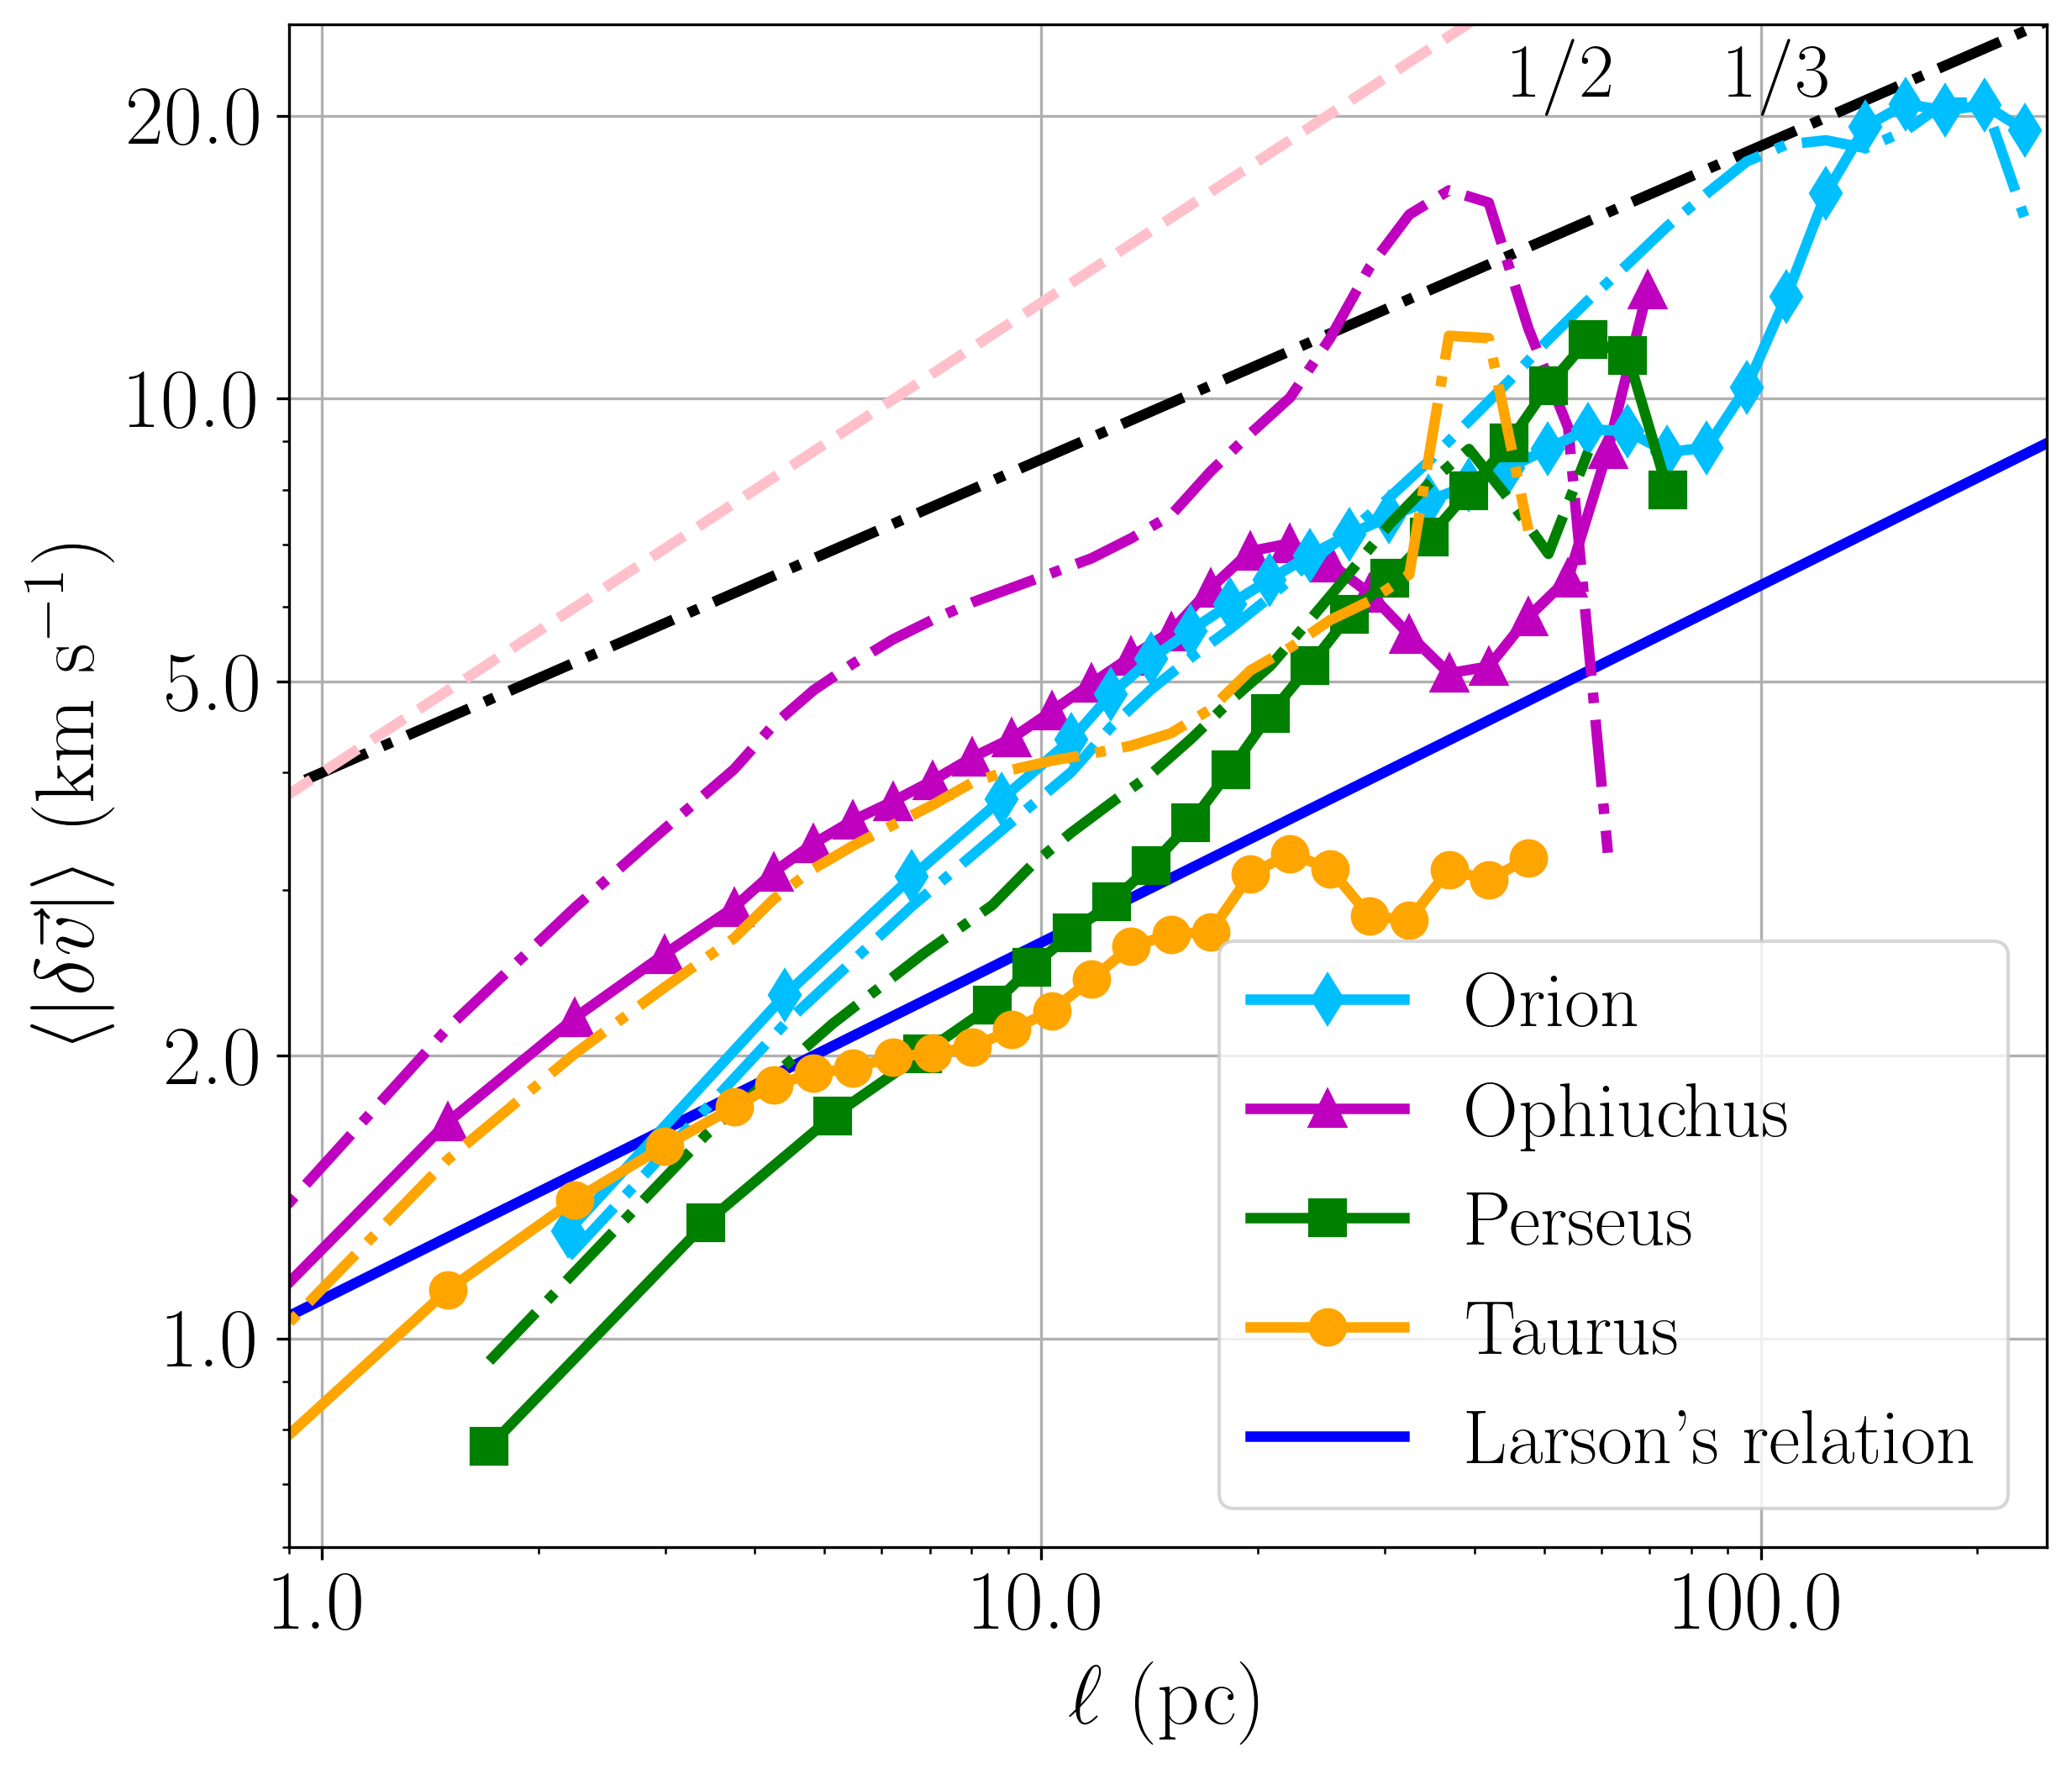
\includegraphics[width=\linewidth]{Stars_img/emission_test.png}
    \caption{VSF of four regions traced by \halpha. Solid lines denote the VSF computed for pixels with low emission, and dotted-dashed lines denote the VSF computed for pixels with high emission.}
    \label{fig:emission}
\end{figure}

Within each individual region, we divide the pixels in half based on the \halpha~brightness---the high-emission half with all the pixels brighter than the median and the low-emission half with all the pixels dimmer than the median. Figure \ref{fig:emission}~shows the VSFs of high-emission \halpha~(dotted-dashed line) and low-emission \halpha~(solid line) within each region. In general, the VSF of high-emission \halpha~has a higher amplitude compared to that of the low-emission \halpha\ component.

One possible explanation for this is that bright \halpha~comes from photo-ionization by young massive stars \citep{tacchella_hensuremathalpha_2022}. Therefore, it traces the most intense stellar feedback regions and shows a higher VSF amplitude. Whereas the low-emission \halpha~comes primarily from collisional ionization. Note that Orion has its high- and low-emission \halpha~ VSFs essentially overlapping for the most part. This is likely because star formation in Orion is the most intense among all the regions studied here \citep[see Table 2 of][]{lada_star_2010}, and thus most of the \halpha~is photo-ionized by massive stars.

There are many uncertainties and potential biases associated with the \halpha~analysis. One source of uncertainty comes from the resolution limit. Although the WHAM data cubes is sampled every 0.25\textdegree, the reported spatial resolution of the survey is 1\textdegree~\citep[][]{haffner_wisconsin_2003}. At separations $\theta \leq 1$\textdegree~(or $\ell_{\rm proj} \leq d \cdot 1$\textdegree), we treat the VSF traced by \halpha~as unresolved (represented by the unconnected dots in Figure \ref{fig:stars_gas}). We note that resolution limit might not significantly alter the overall VSF, as suggested by \citet{li_direct_2020}. Future studies with mock simulated \halpha~observations may help properly evaluate the effects of the resolution limit of the dataset. 

There are also uncertainties with the distance to the \halpha~gas. The bright \halpha~emissions in Orion and Ophiuchus~are likely associated with the star forming regions. However, since Perseus and Taurus do not emit intense \halpha~(see top right panel of Figure \ref{fig:allsky}), it is uncertain whether the centroid velocities found in these two regions are at the exact same distance as the stars.

Another bias can come from the projection effects. When analyzing the VSF of \halpha, we assume that all the gas is located at the same distance, effectively treating it as a 2D structure. This can flatten the VSF for thick clouds, as is discussed in detail in \citet{qian_new_2015, xu_projected_2020, mohapatra_velocity_2022}. All the \halpha~VSFs in our analysis are either as steep as 1/3 or steeper. This suggests that either most of the \halpha~comes from a thin sheet of gas, or the true VSF has an even steeper slope.

Another potential bias related to projection is that we are trying to infer 3D turbulence using projected 2D information. This can introduce uncertainties as the ISM is magnetized. In the presence of magnetic fields, turbulence is no longer isotropic \citep{seifried_impact_2015, hu_anisotropic_2021}. We find that our results are not sensitive to the rotation model (see detailed discussions in Section~\ref{sec:rotation}). 

\subsubsection{The Complex Nature of ISM Turbulence}
\label{sec:nature_ISM}

The ISM is multiphase in nature. The kinematic coupling between these phases is not well understood \citep[for a review of the multiphase ISM model, see][]{cox_three-phase_2005}. More specifically, it is suggested that each phase possesses varying levels of turbulence, where ionized gas has been observed to have higher velocity dispersion than molecular gas in both high- and low-redshift galaxies \citep[][]{girard_systematic_2021,ejdetjarn_giant_2022}. In our study, we observe a similar trend comparing the VSF of \halpha~and other tracers of turbulence.

In Orion and Ophiuchus, there is a large deviation between the level of turbulence seen by different tracers. The VSFs traced by \halpha~show the largest amplitude at large scales, followed by the VSFs traced by stars, and finally by CO\@. One possible explanation is the difference in the transport of energy and momentum from SNe into different phases in these regions, as mentioned in Section \ref{subset:eachregion_result}. In an inhomogeneous medium such as the Milky Way ISM, SNe carry shocked matter radially outward following the path of least resistance. As a consequence, the cool dense phase traced by CO receives less energy injection than the warm diffuse phase traced by \halpha, resulting in lower levels of turbulence in the corresponding VSF\@. Such behavior is also seen in hydrodynamical simulations of single SN remnants \citep[e.g.,][]{martizzi_supernova_2015,li_supernova_2015}.

In Perseus and Taurus, the VSFs traced by \halpha~and CO show a good agreement in both the amplitudes and slopes in these regions, except for the range $\ell \lesssim 7$~pc in Perseus, which suffers from projection effect due to the thickness of the cloud \citep[see Section 4.2 of][for a detailed discussion]{qian_new_2015}. At larger $\ell$, the VSF traced by \halpha~and stars also closely follow each other. Such trend is consistent with the evolutionary history of these regions with no clear imprint of recent SN explosions. Without this important local driver of turbulence, different phases of gas are well-coupled, and the young stars formed out of these molecular clouds also largely retain the same memory of turbulence. 

At length scales beyond the bumps caused by SN energy injection, we recognize a common upward trend in the VSFs of stars. In all four regions, the VSFs at the largest $\ell$~maintain a positive slope with no apparent driving scale. At these length scales, the ISM turbulence is driven primarily by galactic shear \citep[see, e.g.,][]{gammie_velocity_1991} and accretion flows onto the galaxy \citep[][]{forbes_gas_2023}.

The difference of \halpha~VSFs in different regions show that ISM turbulence can be unevenly distributed spatially as a result of local drivers. Turbulence can also be unevenly distributed between different phases of the ISM (e.g., Orion and Ophiuchus). Section~\ref{sec:halpha_discussion} and Figure~\ref{fig:emission} further demonstrate that even with the same gas tracer \halpha, the level of turbulence can vary depending on its brightness. In addition, we note that local energy injection from supernova explosions is also intermittent temporally. Using the \halpha~VSF in Ophiuchus, we estimate the eddy turnover time at the driving scale to be:
\begin{equation}
\frac{\ell}{v}\sim \frac{20\text{--}30\,\mathrm{pc}}{5\,\mathrm{km\,s^{-1}}}\sim 4\text{--}6\,\mathrm{Myr}.
\end{equation}
The \halpha~VSF in Orion gives a similar estimate. Typically, it takes a few eddy turnover times to establish a steady-state turbulent flow. On the other hand, given the size of these regions, the average time interval between supernovae is on the order of a few Myr \citep{narayan_pulsar_1990, li_supernova_2015}. Each event also injects energy as a pulse with a very short duration. Therefore, both the ``on'' and ``off'' states of the driver are short compared with the timescale required to achieve a steady state. Thus ISM turbulence in molecular complexes is often not in a steady state.


\subsection{Conclusions} \label{sec:conclusions}

In this work, we analyze the kinematics of young stars and gas in four nearby star-forming regions: Orion, Ophiuchus, Perseus, and Taurus. For each region, we compute the first-order VSF of young stars and \halpha~gas, and compare the results against each other, as well as analysis of CO molecular cores from the literature.

We find that the VSFs traced by young stars in all four regions exhibit similar properties largely in agreement with Larson's relation and reveal a universal scaling of turbulence in the ISM\@. This also confirms our previous finding in \citet[][]{ha_measuring_2021} that young stars retain the memory of turbulence in their natal molecular clouds, and thus can be used to measure the turbulent kinematics of molecular clouds.

The VSFs of \halpha~are more diverse, likely as a result of local energy injection. In regions with recent SN activities such as Orion and Ophiuchus, the VSFs of \halpha~are higher in amplitude compared to those without. The \halpha~VSFs are also higher than the VSFs of stars and CO in these regions, while regions without recent SN explosions (Perseus and Taurus) show well-coupled turbulence between different phases. Within each individual region, the high-emission \halpha~tends to show higher VSFs than the low-emission \halpha.

Our findings support a complex picture of the Milky Way ISM, where turbulence can be driven at different scales and inject energy unevenly into different phases. Future observations with more tracers of turbulence and on more star forming regions will help us better understand the diversity and complexity of ISM turbulence. In addition, high-resolution numerical studies can help further our understanding of the coupling between different phases and relevant timescales.


\subsection{Supplemental Material}

\subsubsection{Selection of the \texorpdfstring{\rophi}{rho Oph}~dark cloud within the Upper Sco region}
\label{sec:Upper_Sco}

\begin{figure}
    \centering
    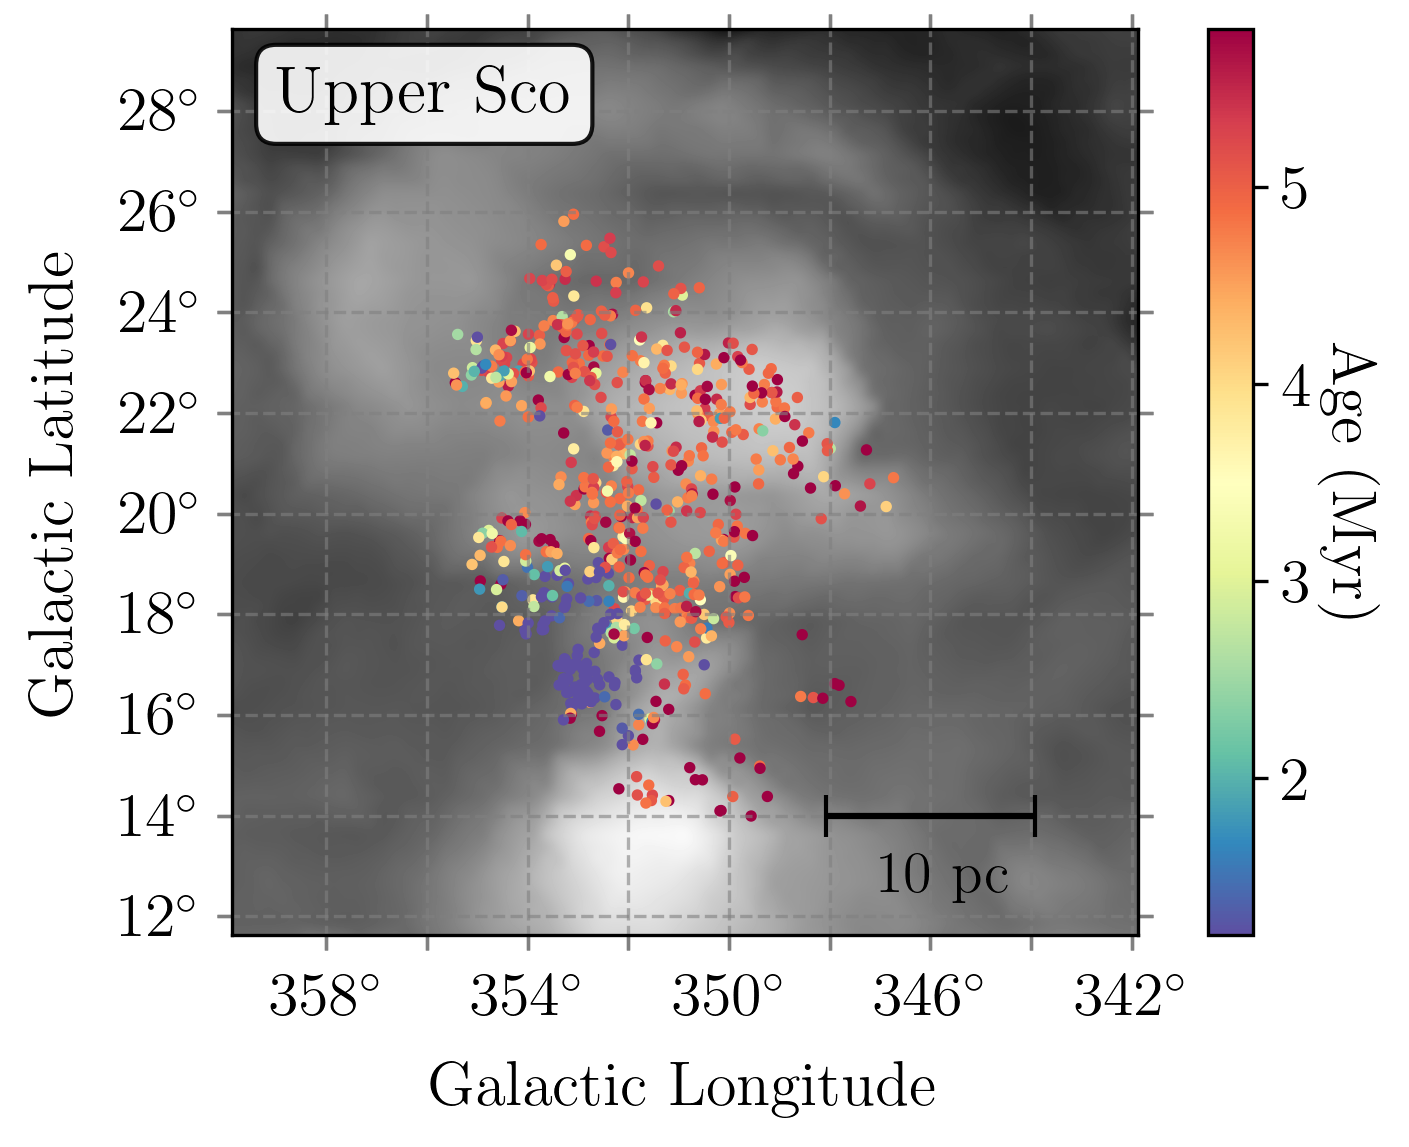
\includegraphics[width=0.7\columnwidth]{Stars_img/UpperSco_age.png}
    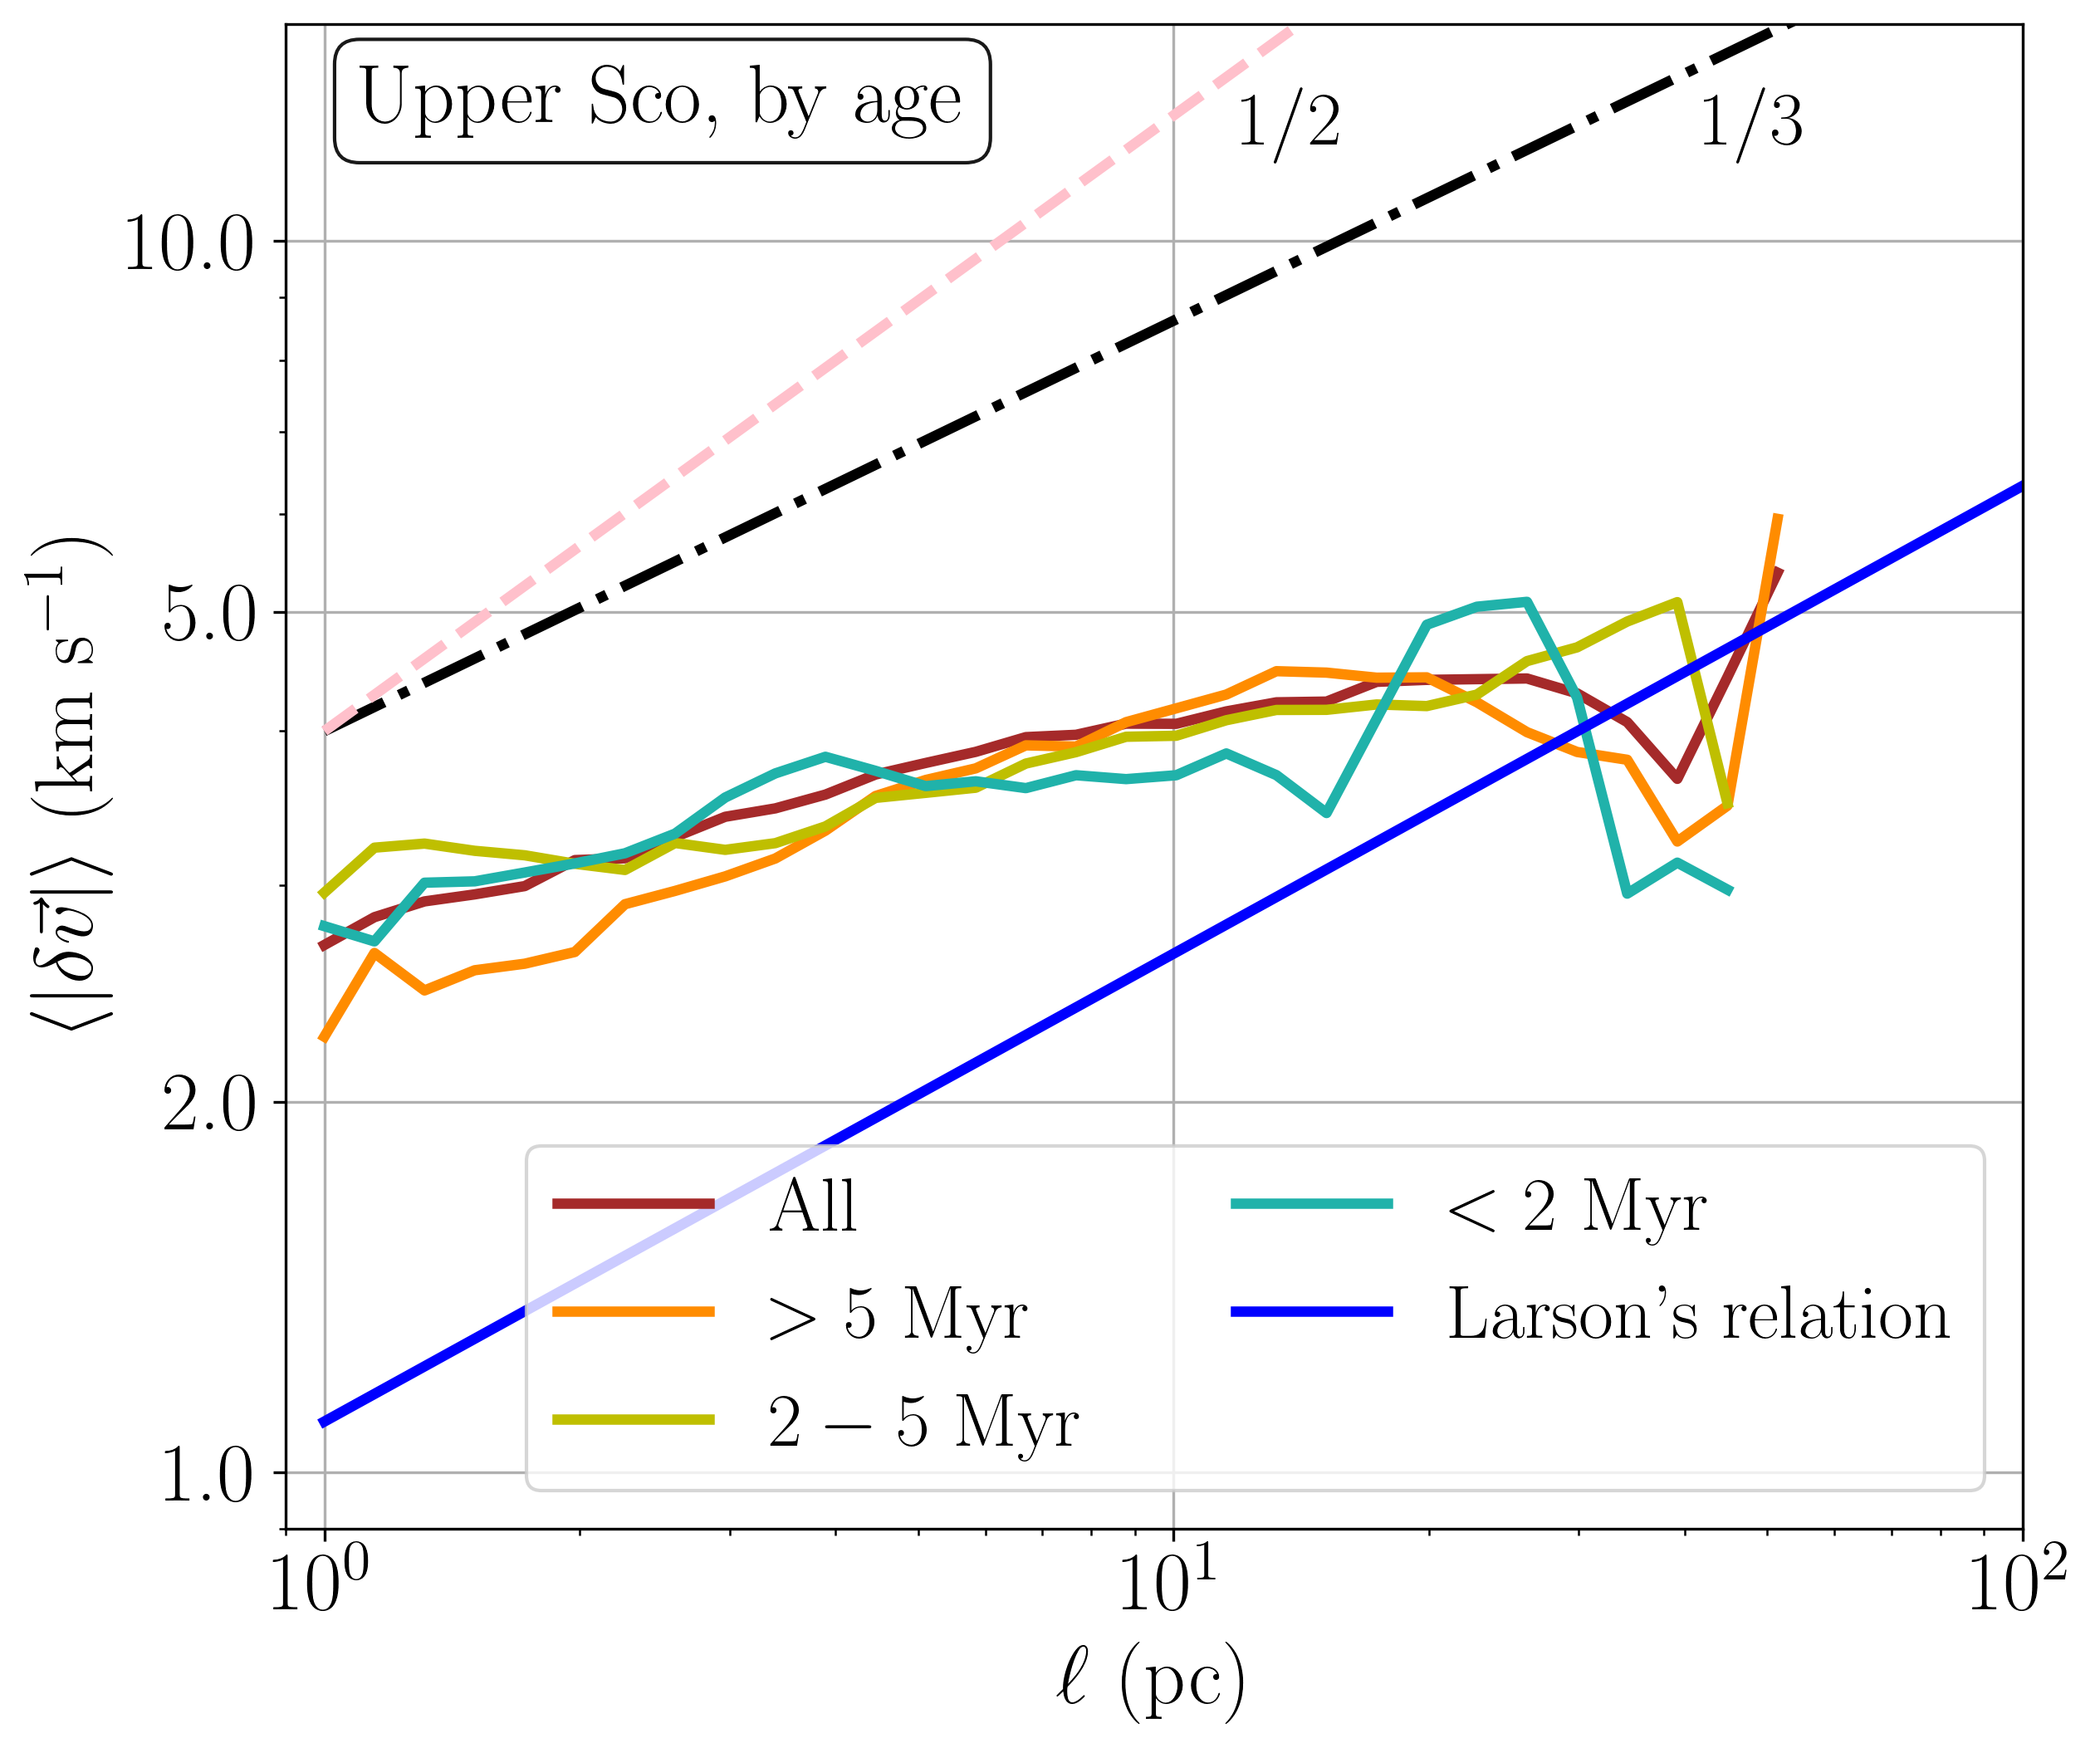
\includegraphics[width=0.7\columnwidth]{Stars_img/UpperSco_age2_vsf.png}
    \caption{Top panel: positions of young stars color-coded by their age. Stellar age is estimated using the Sagitta package developed by \citet{mcbride_untangling_2021}. Background shows \halpha~flux from the WHAM survey. Bottom panel: the VSF of stars in Upper Sco within three age brackets. Only stars younger than 2 Myr show characteristic of SN energy injection.}
    \label{fig:uppersco_age}
\end{figure}
In the main body of this paper, we select only stars within the actively star-forming region Ophiuchus. Here, we show the analysis results when selecting the entire Upper Sco region and discuss how the VSF of the stars depend on the stellar age.

The top panel of Figure \ref{fig:uppersco_age}~shows the spatial distribution of stars in Upper Sco and their age. Most of the stars outside Ophiuchus~are older than 4 Myr, while stars inside Ophiuchus~are much younger, primarily younger than 2 Myr. The SN explosion in this region traced by runaway stars took place $\sim 2$~Myr ago \citep[][]{neuhauser_nearby_2020}, so the majority of stars in Upper Sco did not receive energy injection from this event, and thus would not exhibit characteristics of such energy injection in their VSF\@. Indeed, we see this trend in the lower panel of Figure \ref{fig:uppersco_age}. With the entire Upper Sco region taken into account, the VSF shows only a slight bump at $\sim 25$~pc, while both the VSF of stars older than 5 Myr and of stars between 2 and 5 Myr do not show any discernible energy injection scale. Meanwhile, the VSF of stars younger than 2 Myr shows a clear energy injection scale at $\sim 25$~pc, similar to what we obtain in the main paper. Because of these results, we elect to use only stars categorized as members of Ophiuchus, the majority of which are younger than 1 Myr, for the analysis in the main body of this paper.


\subsubsection{Effect of Galactic Rotation on the VSF of \texorpdfstring{\halpha}{H-alpha}}
\label{sec:rotation}

\begin{figure}
    \centering
    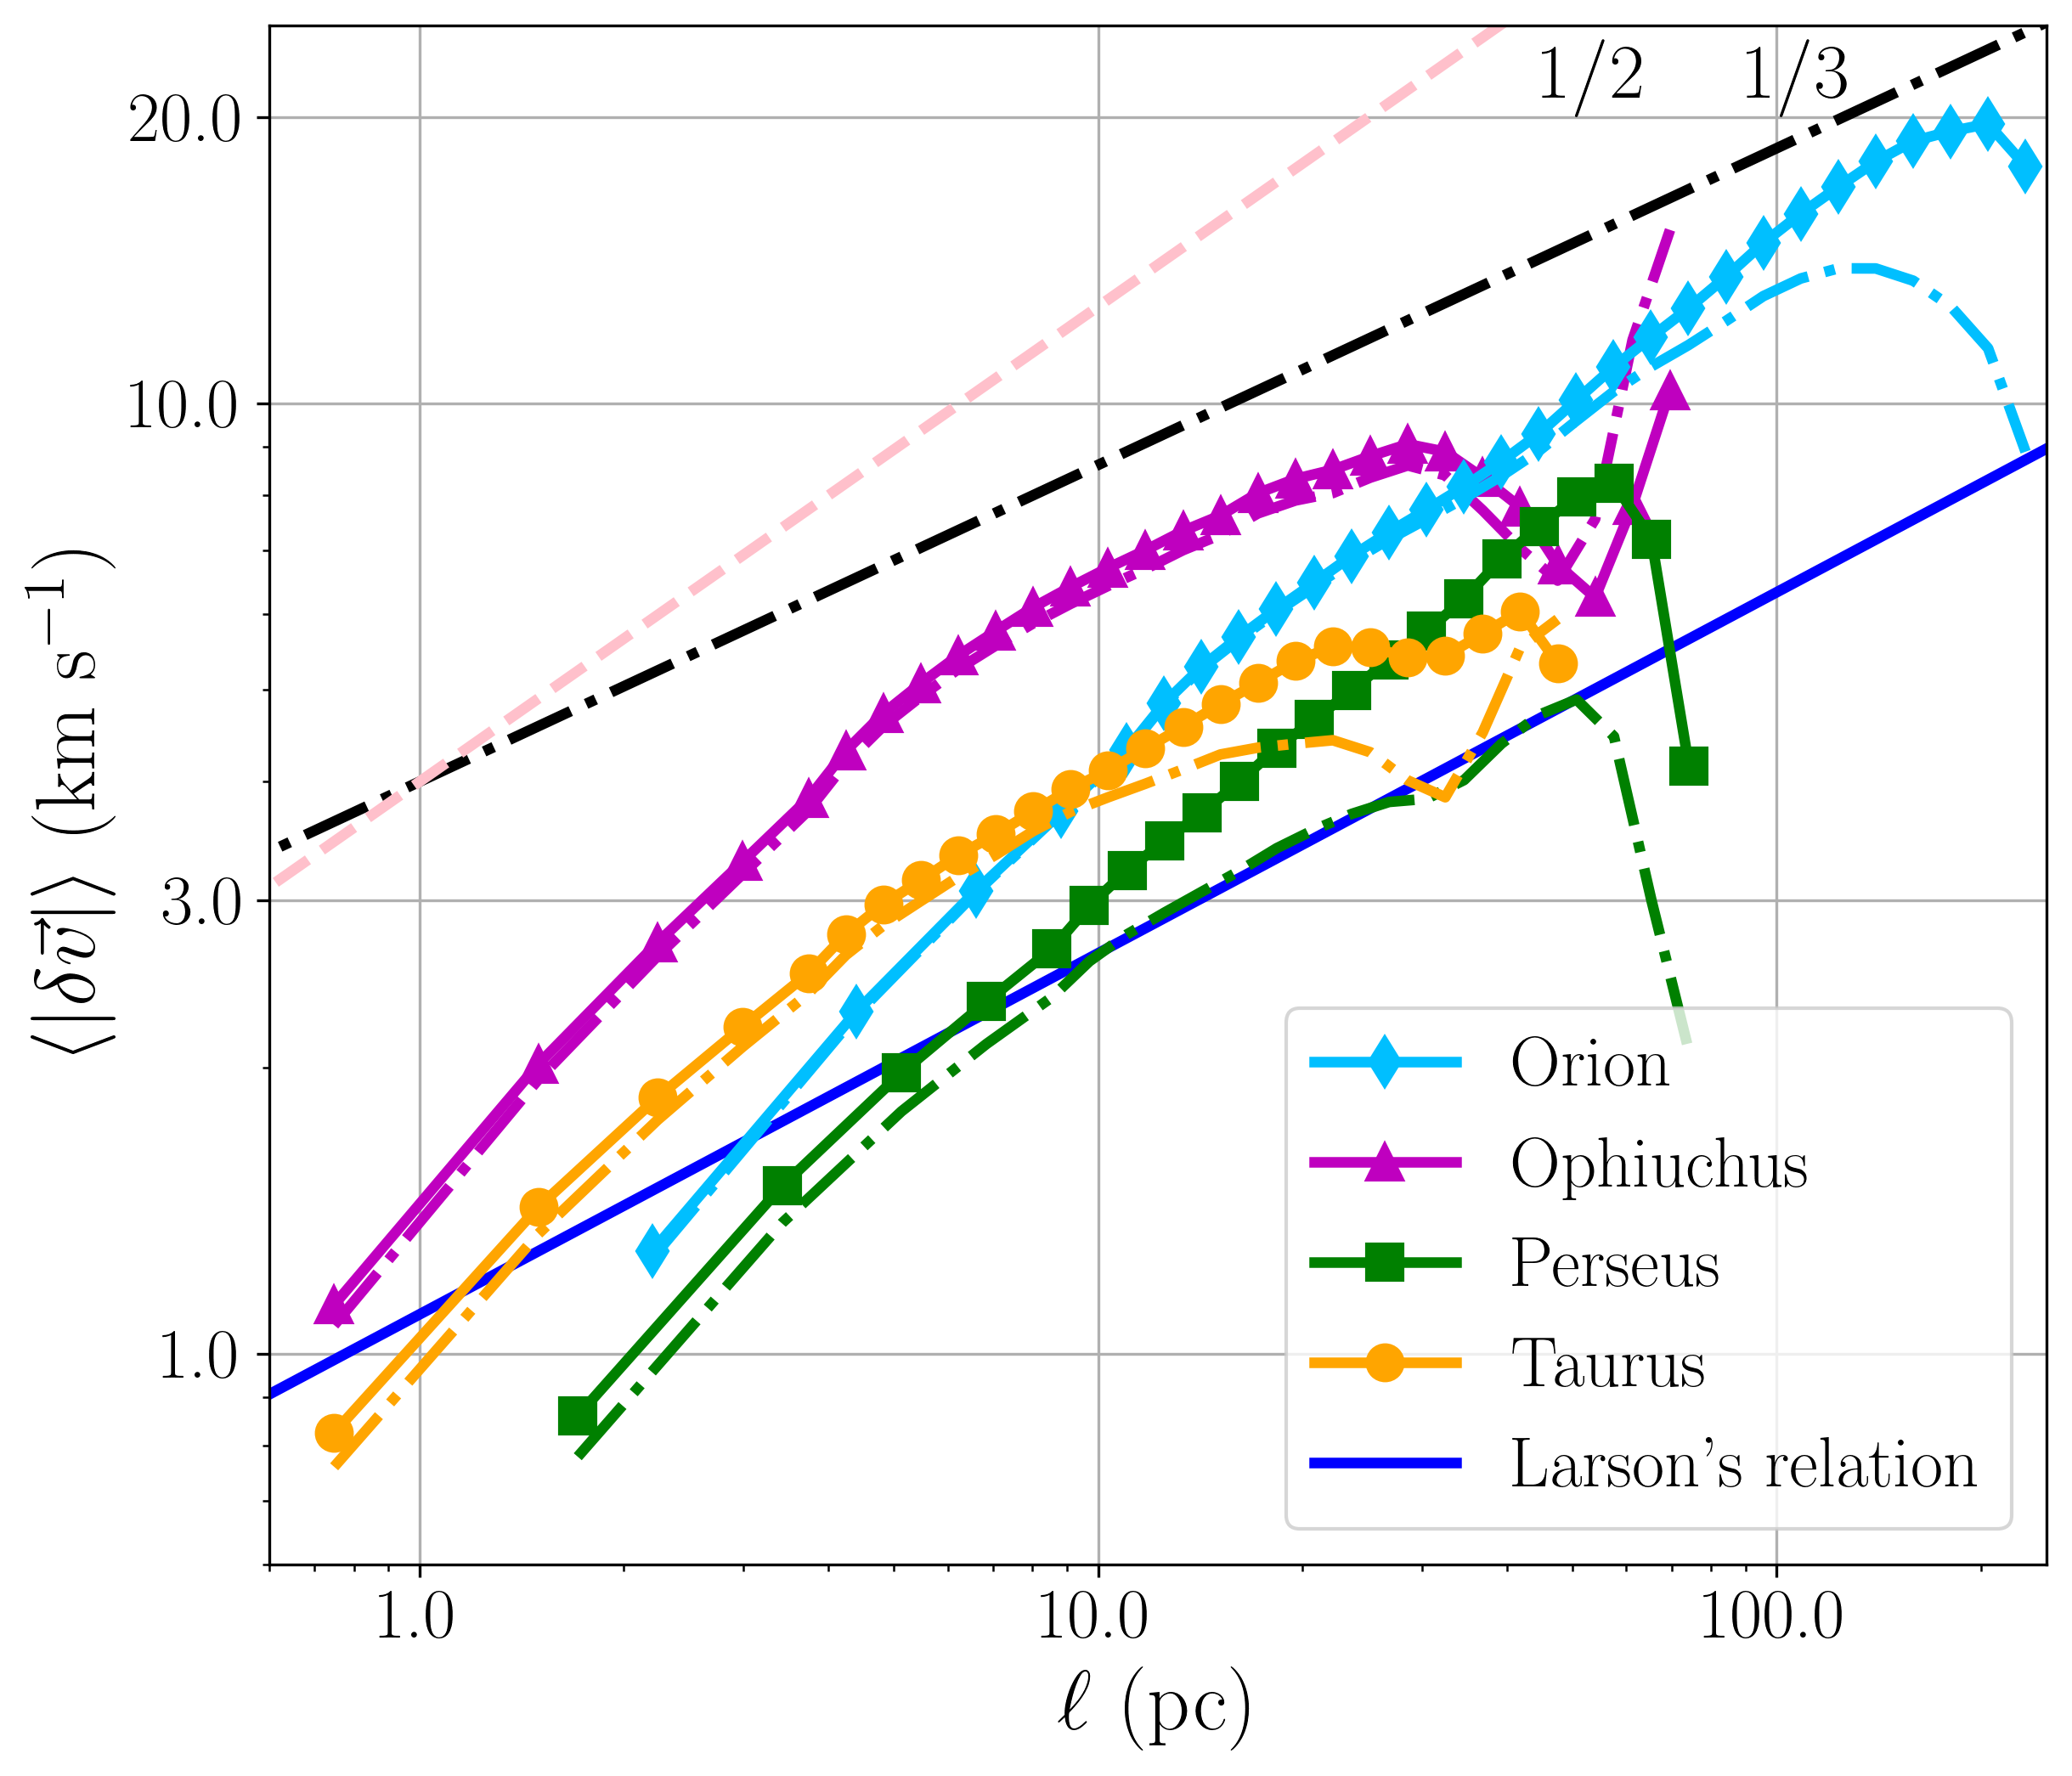
\includegraphics[width=\columnwidth]{Stars_img/test_rotation.png}
    \caption{The VSFs of \halpha, with (solid lines) and without (dotted-dashed lines) a correction to the Galactic rotation \citep{qu_warm_2020}.}
    \label{fig:rotation}
\end{figure}

Figure \ref{fig:rotation} shows the VSF traced by \halpha~in four regions with and without Galactic rotation correction. In three out of the four regions, when a rotation profile is applied, the VSF does not significantly differ from the VSF without a rotation correction up to $\sim 20$~pc. This behavior is expected, since at small $\ell$ the rotation corrections between two points are very similar. Thus, $\delta \vec{v}$ between two points essentially cancels out the rotation correction, and the shape of the VSF is preserved. For two points separated by a large distance, the rotation correction applied to them can differ more, and hence results in a shift in the VSF, as Figure \ref{fig:rotation} shows. However, the overall shifts in the VSFs due to rotation correction are moderate and do not affect the conclusions of our work. 

\subsubsection{Effect of the size and location of the \texorpdfstring{\halpha}{H-alpha}~window}
\label{sec:windowsize}

\begin{figure*}[ht]
    \centering
    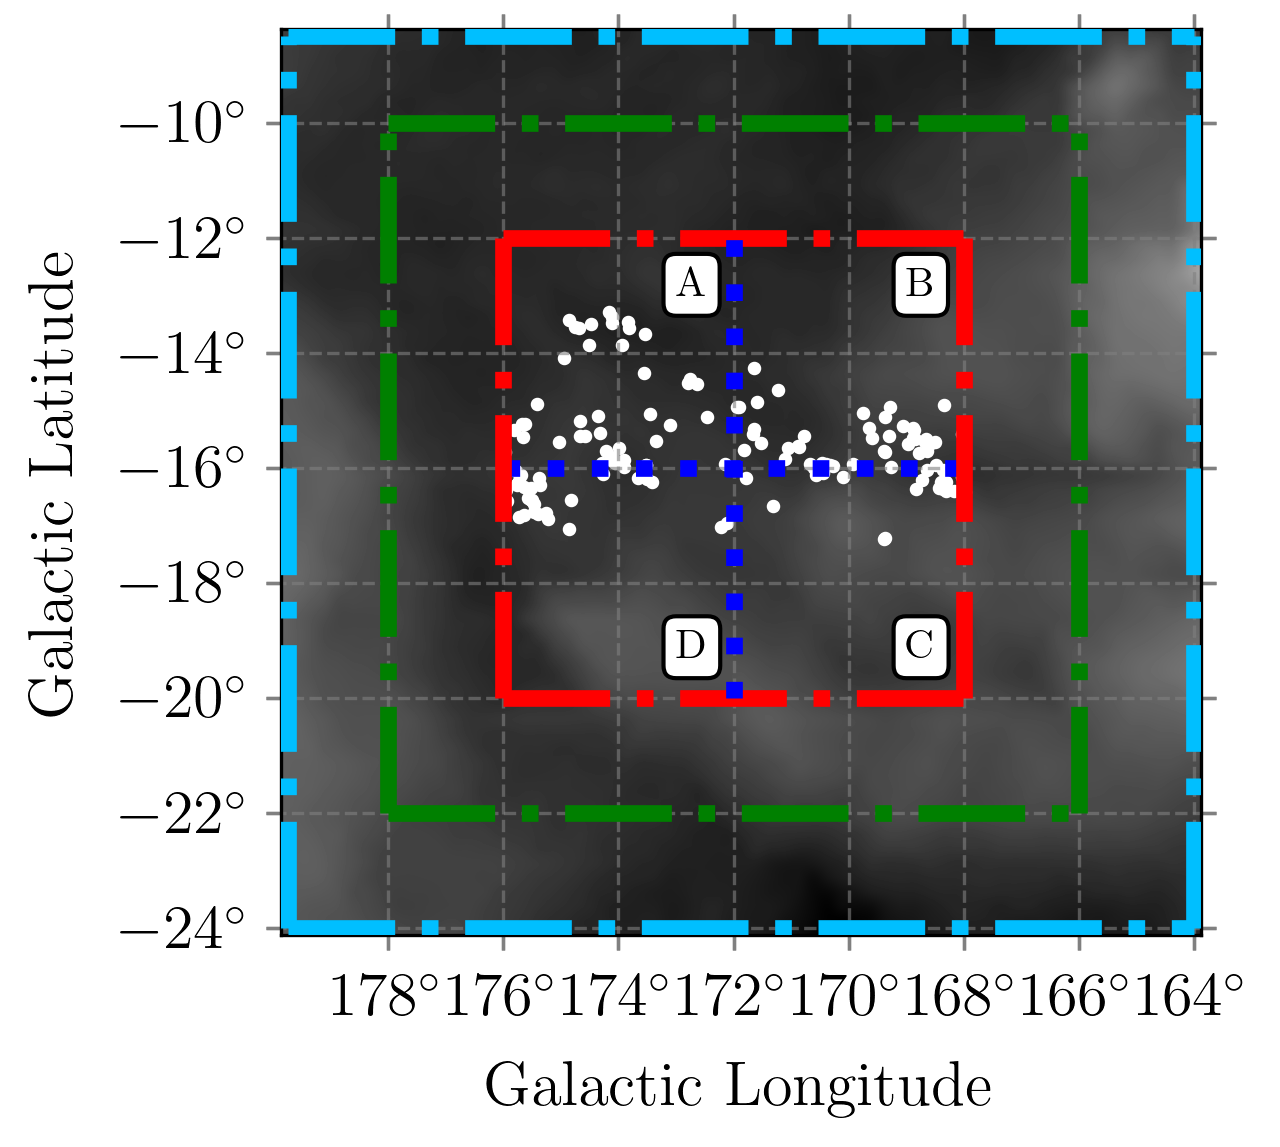
\includegraphics[width=0.5\linewidth]{Stars_img/tau_illustration.png} \\
    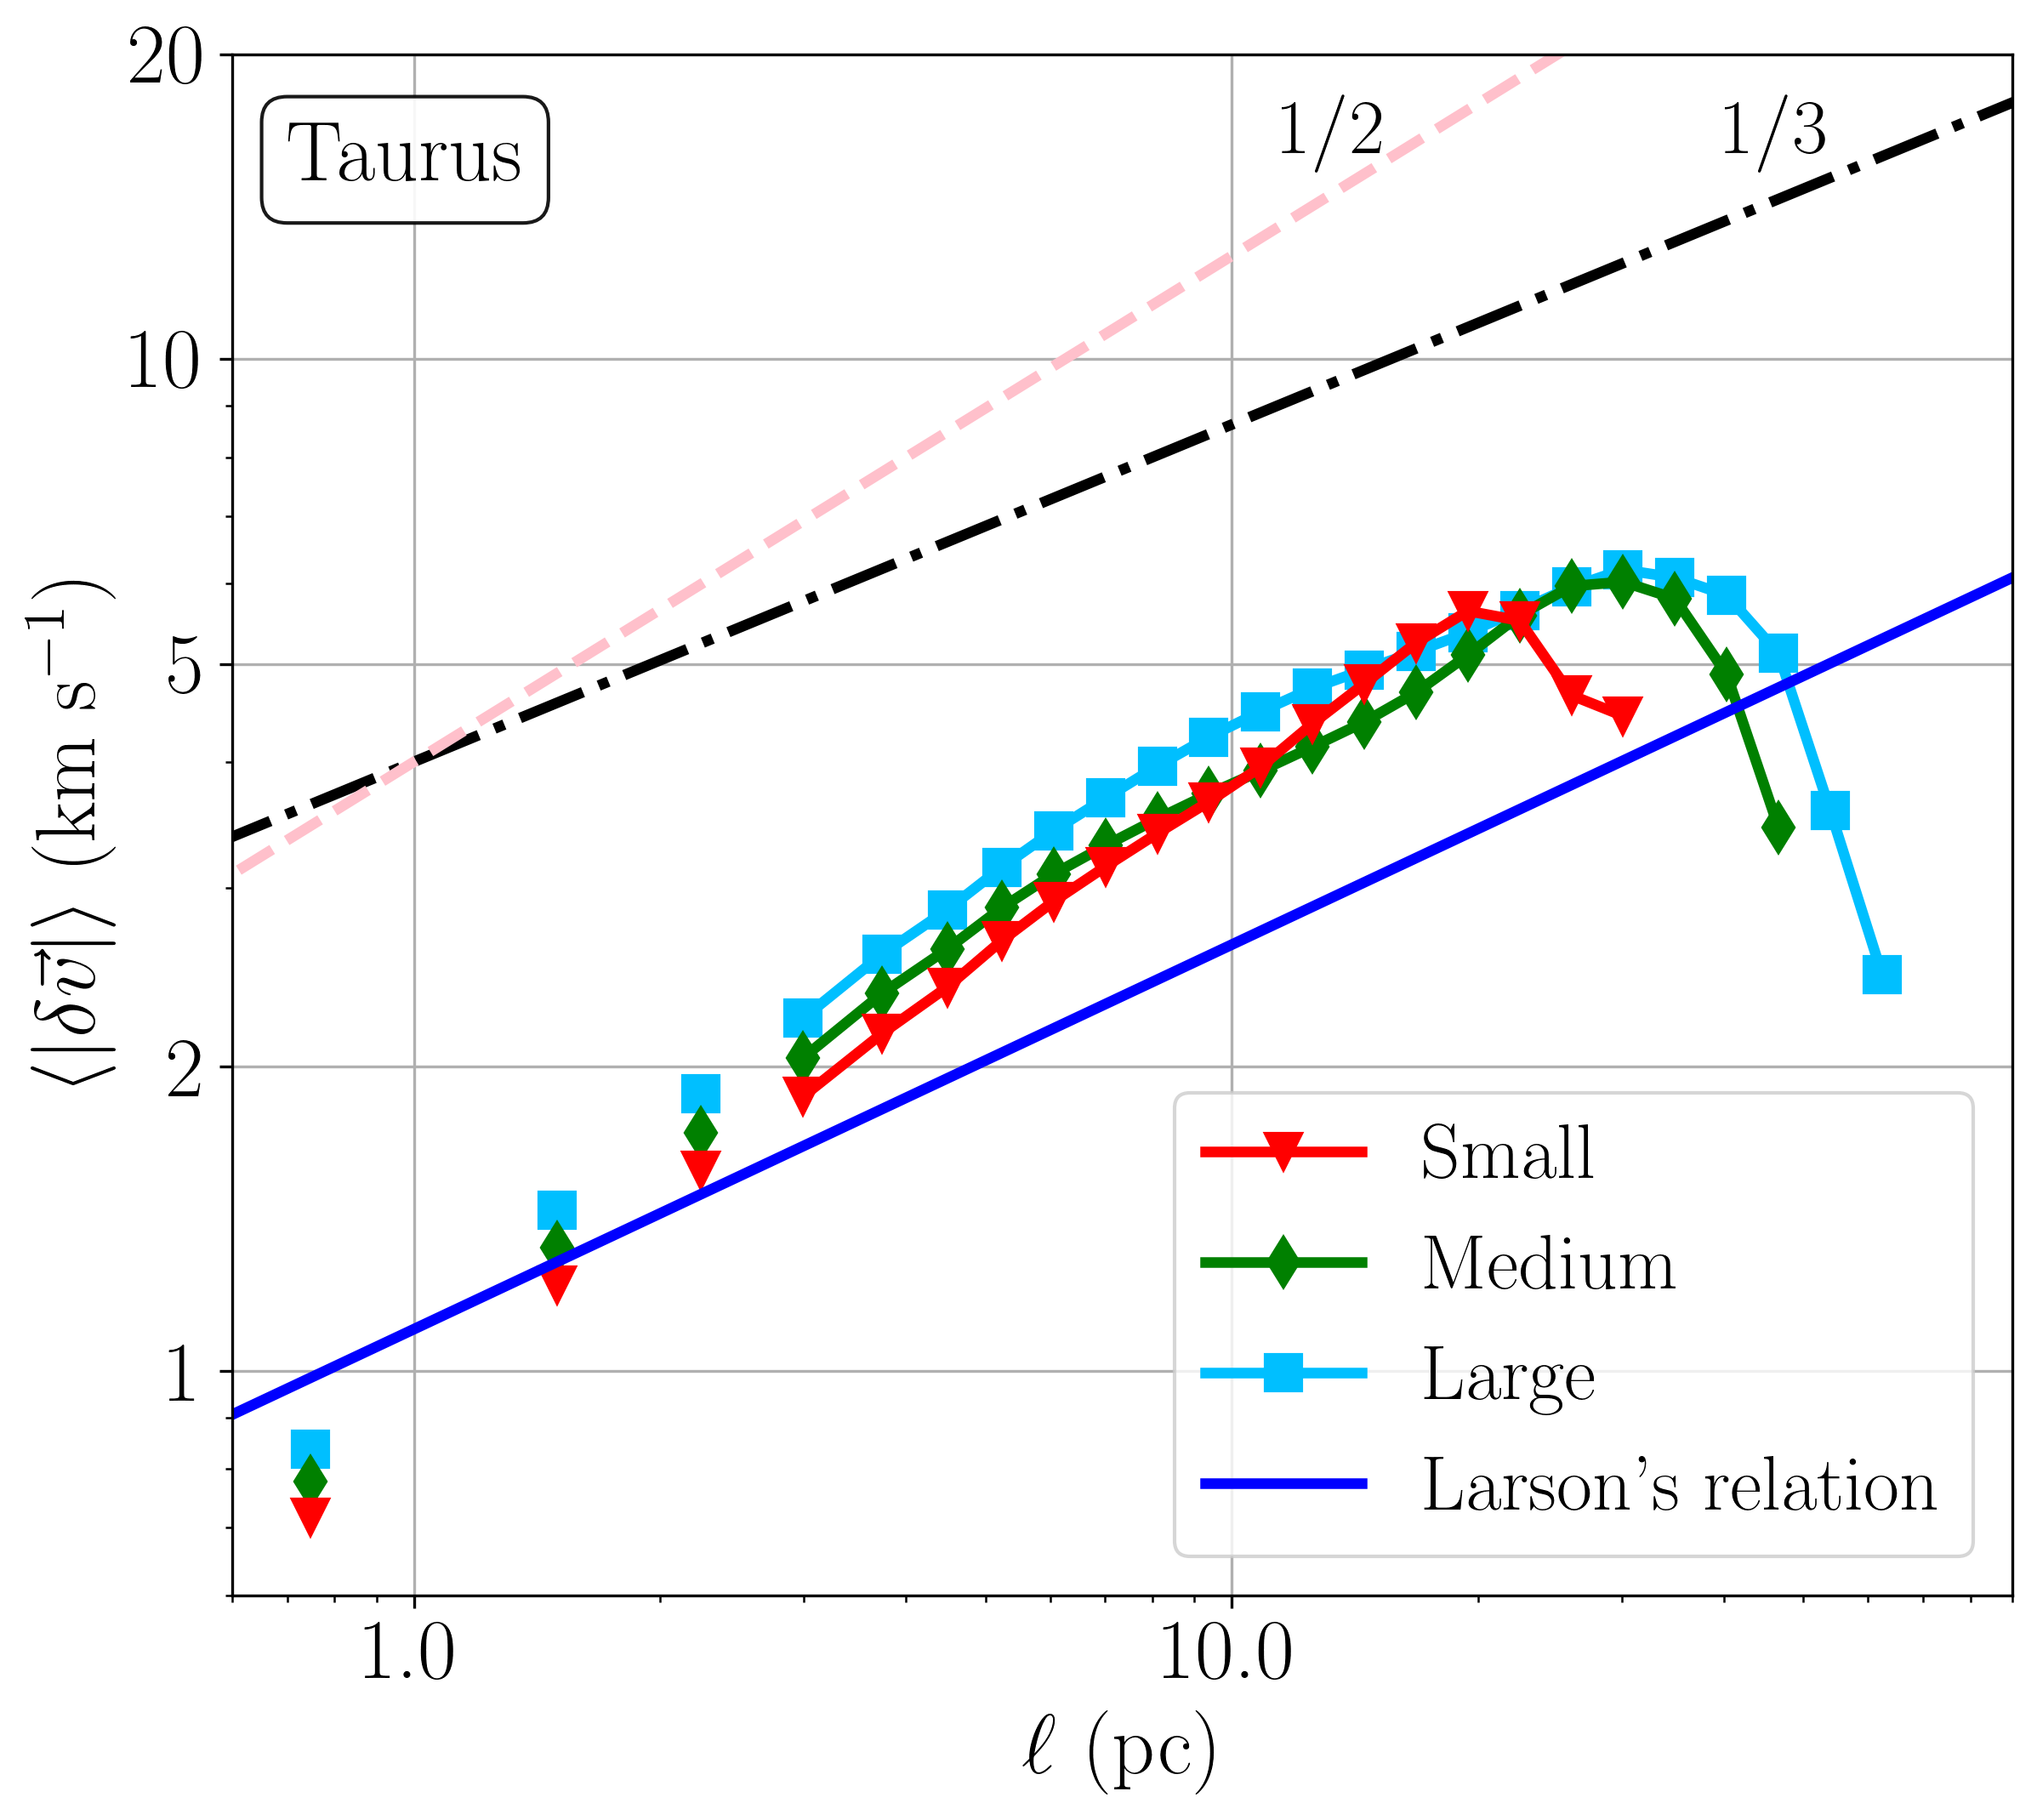
\includegraphics[width=0.45\linewidth]{Stars_img/different_size_test_tau.png}
    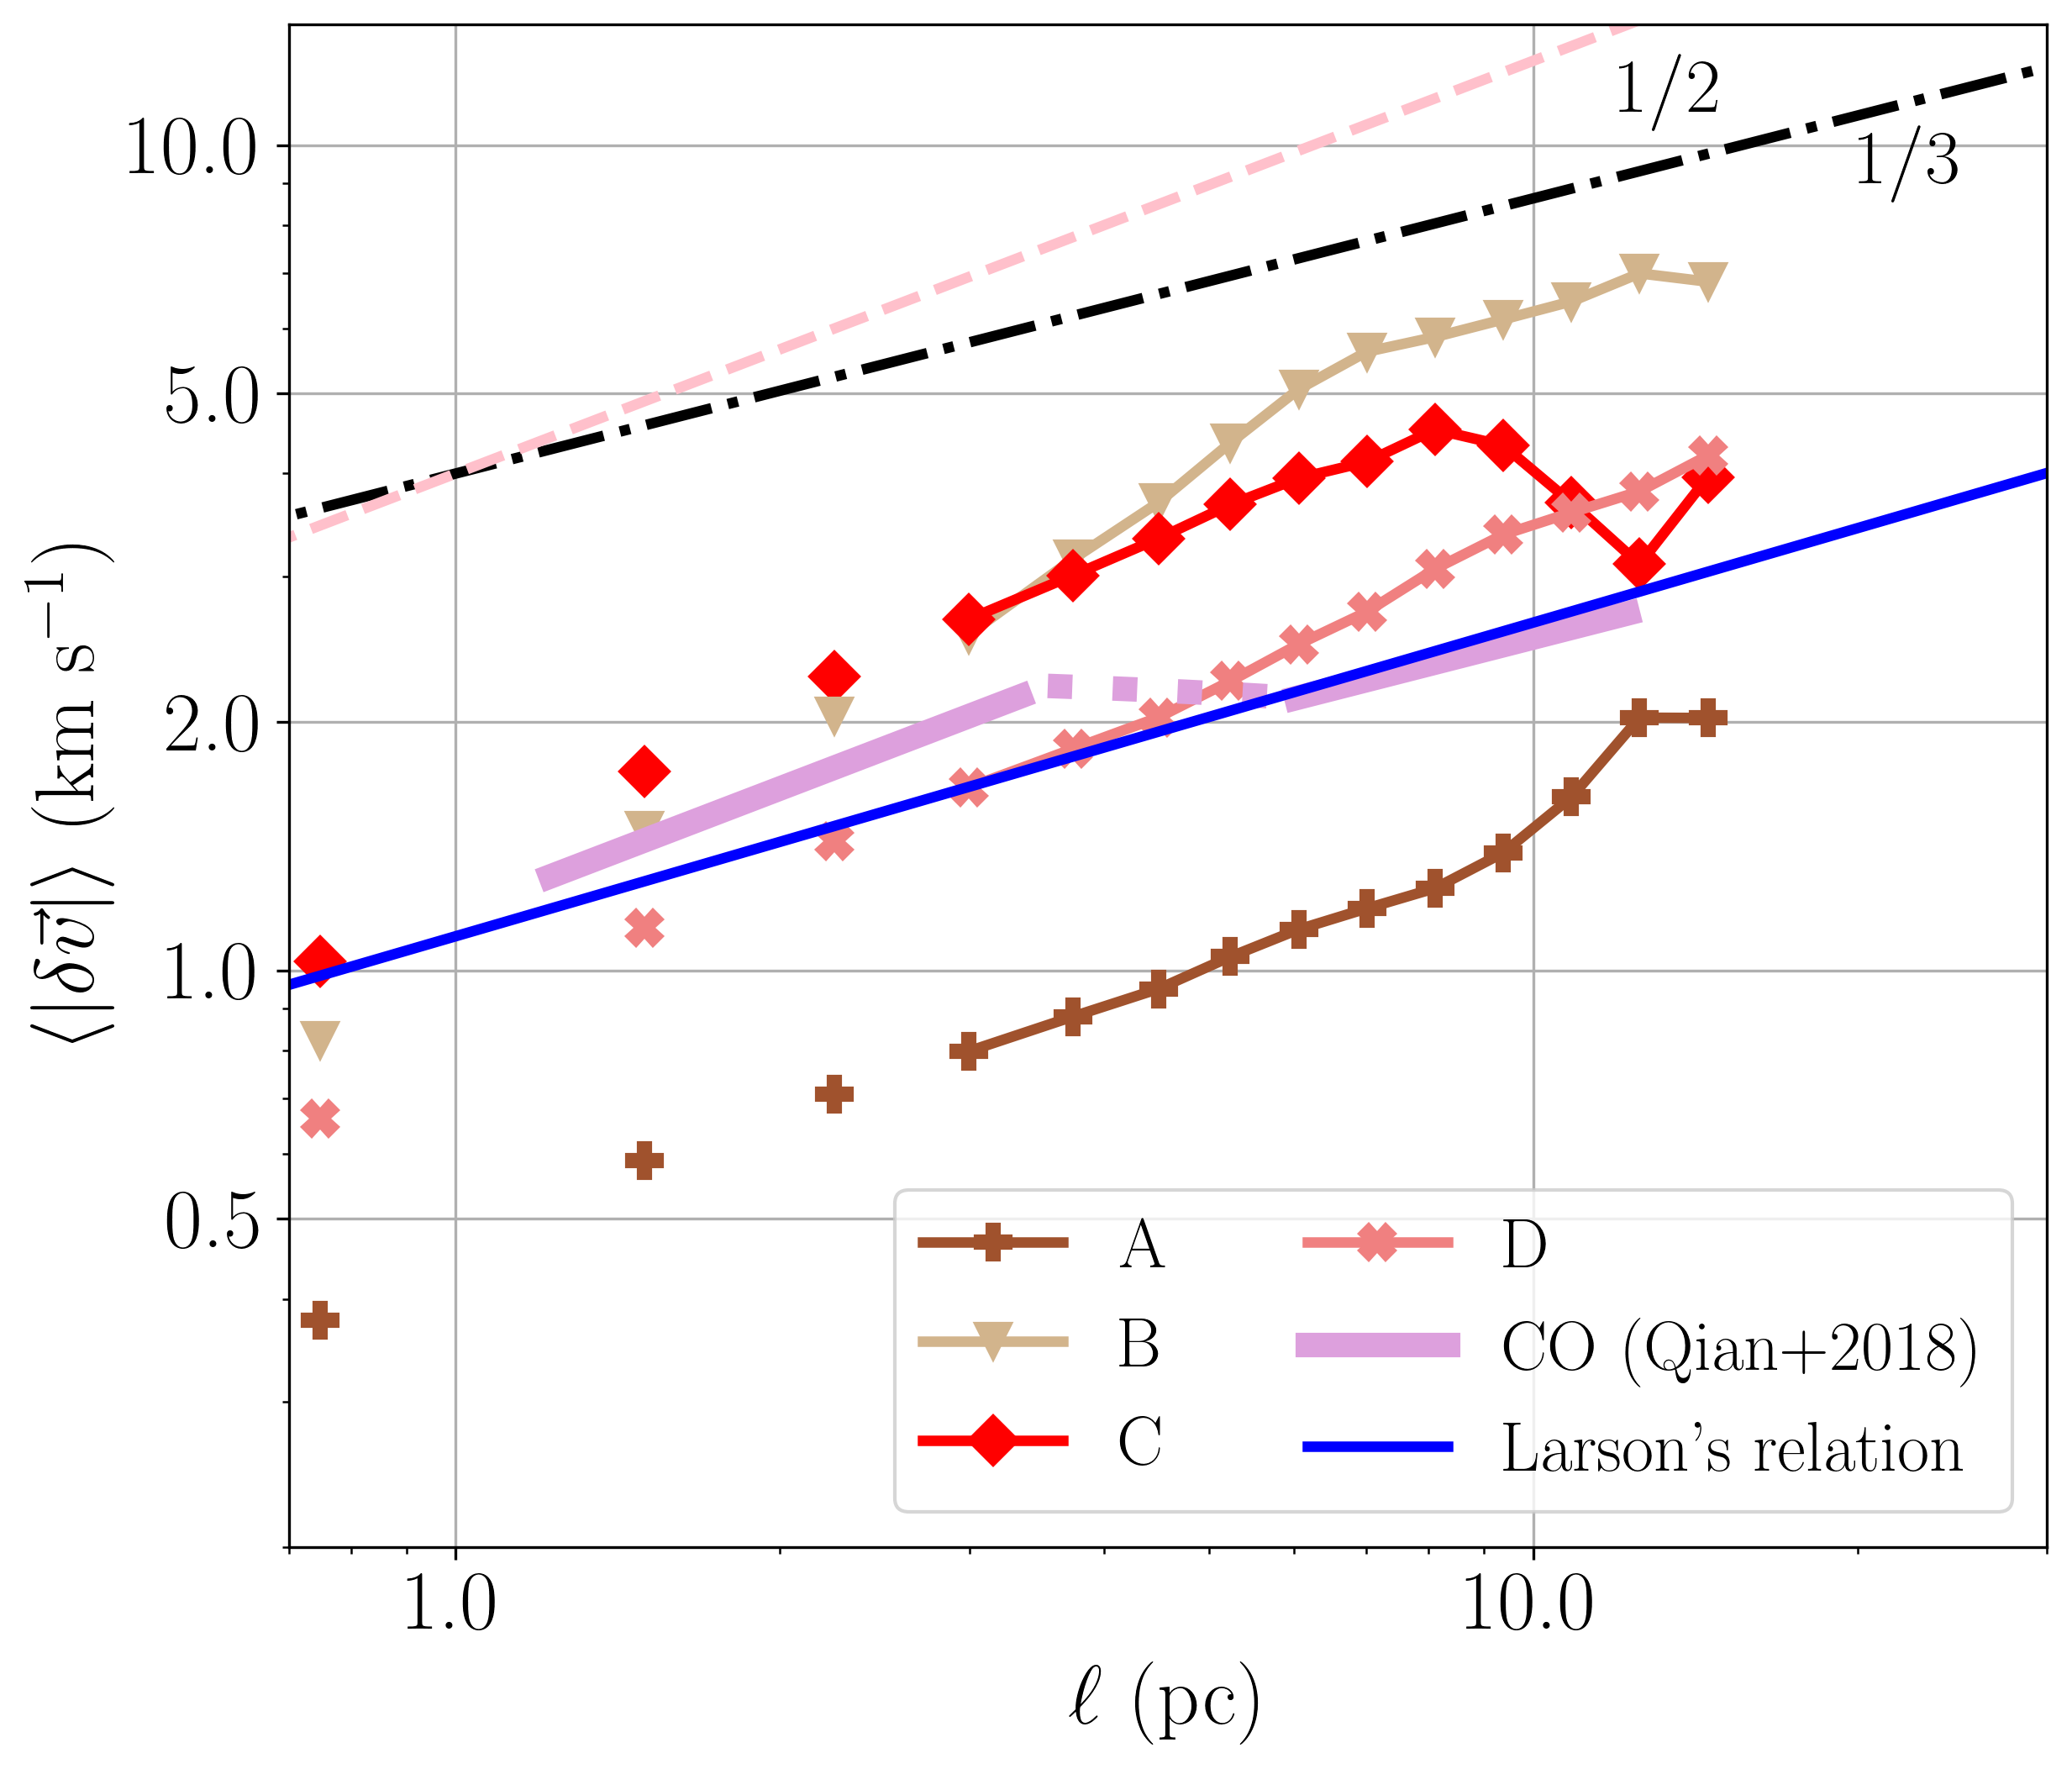
\includegraphics[width=0.46\linewidth]{Stars_img/same_size_test_tau.png}
    \caption{Top panel: illustration of our \halpha~window tests. The red box is the smallest window within which all stars in Taurus belong. The two boxes in green (the window used in the main analysis) and light-blue are each 4 deg$^2$~bigger than the former. Inside the red box, we also test the variation of the VSF within the region by dividing the window into four equal-sized boxes. Bottom left panel: The VSF of Taurus traced by \halpha, plotted across three different window sizes.
    Bottom right panel: The \halpha~VSFs of Taurus in the four quadrants within the red window. }
    \label{fig:aperturesize}
\end{figure*}

Another potential source of bias comes from the exact size and location of the window chosen to calculate the VSF of \halpha~within each region. In Section \ref{subset:eachregion_result}, we caution that the bumps seen in the VSF of \halpha~are potential artifacts since they are close to the size of the window. Such an effect is noted as the apparent driving scale in simulations of multiphase turbulence, and is equal to 1/2 of the box size \citep[e.g.,][]{mohapatra_velocity_2022}. To test whether this effect is also present in the VSF of \halpha, we select a solid angle that encompasses all the stars in a region, and compute the VSF within this window. We then compute the VSF for a window that is 4 deg$^2$ larger, and repeat this a second time (see top panel in Figure~\ref{fig:aperturesize}).

In all four regions, the VSFs of \halpha~are independent of the window size up to $\ell \sim L/2$, where $L$ is the window size. In Taurus and Perseus, the bump in the VSF shifts to larger $\ell$ when the window size increases. Thus we conclude that in these regions, the VSF bump is likely caused by the box limit rather than a real physical driving scale. As an example, the bottom left panel of Figure \ref{fig:aperturesize} shows the VSF of \halpha~in Taurus as a function of window size. 



We also use Taurus as an example to illustrate the spatial variation of turbulence on small scales. We divide the smallest box (8 deg$^2$) in the previous experiment into four equal-sized quadrants. The bottom right panel of Figure \ref{fig:aperturesize} shows the \halpha~ VSFs of these four quadrants in Taurus. Although the slopes of these four VSFs are roughly consistent with one another, their amplitudes vary by up to a factor of three, indicating potentially large variations in turbulence between local patches of the ISM\@. The VSF of CO is in the best agreement with the bottom-left window ($172^{\circ} < l < 176^{\circ}$~and $-20^{\circ} < b < -16^{\circ}$), where many CO cores were also identified \citep[see Figure 2 of][for detailed locations of CO cores in Taurus]{qian_13co_2012}.
